\documentclass{article}

\usepackage{Stil}
\usepackage[utf8]{inputenc}
\usepackage{amsmath}
\usepackage{amsfonts}
\usepackage{amssymb}
\usepackage{graphicx}
\usepackage{float}
\usepackage{tikz}
\usepackage{listings}
\usepackage{color}
\usepackage{hyperref}
\usepackage{geometry}
\usepackage{tcolorbox}
\usepackage{qrcode}

% Python kod renklendirmesi için
\definecolor{codegreen}{rgb}{0,0.6,0}
\definecolor{codegray}{rgb}{0.5,0.5,0.5}
\definecolor{codepurple}{rgb}{0.58,0,0.82}
\definecolor{backcolour}{rgb}{0.95,0.95,0.92}

 \renewcommand{\abstractname}{Özet}

\lstdefinestyle{mystyle}{
    backgroundcolor=\color{backcolour},   
    commentstyle=\color{codegreen},
    keywordstyle=\color{magenta},
    numberstyle=\tiny\color{codegray},
    stringstyle=\color{codepurple},
    basicstyle=\ttfamily\footnotesize,
    breakatwhitespace=false,         
    breaklines=true,                 
    captionpos=b,                    
    keepspaces=true,                 
    numbers=left,                    
    numbersep=5pt,                  
    showspaces=false,                
    showstringspaces=false,
    showtabs=false,                  
    tabsize=2
}

\lstset{style=mystyle}

\title{Yapısal Optimizasyon Teknikleri}
\author{Bilal TAYFUR}

\begin{document}

\begin{titlepage}
\thispagestyle{empty}
\maketitle

\begin{abstract}
Bu ders, yapısal sistemlerin optimizasyonu konusunda kapsamlı bir giriş sunmaktadır. Öğrenciler, optimizasyon teorisinin temellerinden başlayarak, klasik ve modern optimizasyon yöntemlerinin genel farkını öğrenecek, yapısal sistemlerin tasarımında ve analizinde bu yöntemleri uygulama becerisi kazanacaklardır. 

Anlatılan konuların sağ tarafında verilen karekodlar üzerinden derse ait GitHub reposunda ilgili örneğin kodlarına erişilebilir. Bu repo her yıl güncellenmektedir. Dolayısıyla güncel ders notlarına ve yeni eklenen uygulamalara da repo üzerinden erişlebilir ve arzu edilirse katkı sağlanabilir.

\vspace{10pt}
\begin{center}
\qrcode[height=4cm]{https://github.com/btayfur/structural-optimization}
\end{center}




\vspace{10pt}
\noindent Bu ders kapsamında, aşağıdaki kaynak kitaplar konuları daha derinlemesine incelemek isteyen öğrencilere tavsiye edilmektedir:

\begin{itemize}
    \item Cottle, R. W., \& Thapa, M. N. (2017). \textbf{Linear and Nonlinear Optimization}. Springer.
    \item Rao, S. S. (2019). \textbf{Engineering Optimization: Theory and Practice, 5th Edition}. John Wiley \& Sons.
    \item Arora, J. S. (2016). \textbf{Introduction to Optimum Design, 4th Edition}. Academic Press.
    \item Yang, X. S. (2021). \textbf{Nature-Inspired Optimization Algorithms, 2nd Edition}. Elsevier.
    \item Bendsøe, M. P., \& Sigmund, O. (2003). \textbf{Topology Optimization: Theory, Methods, and Applications}. Springer.
\end{itemize}

\end{abstract}

\setcounter{tocdepth}{3}
\tableofcontents
\end{titlepage}

\newgeometry{top=20mm,bottom=25mm,right=80mm,left=20mm}

% Haftalık içeriklerin dahil edilmesi
\section{Optimizasyon Teorisine Giriş}
Optimizasyon teorisi, bir sistemin performansını belirli kısıtlar altında en iyi duruma getirmeyi amaçlayan matematiksel ve metodolojik yaklaşımların bütünüdür. Bu ders, yapısal sistemlerin optimizasyonuna odaklanarak, temel kavramları ve uygulama yöntemlerini ele alacaktır.

\subsection{Optimizasyonun Tanımı ve Mühendislikteki Önemi}
Optimizasyon, bir sistemin performansını belirli kısıtlar altında en iyi duruma getirme sürecidir. \sidenote{Günlük hayatta sıkça karşılaştığımız "en iyi" kararı verme süreçleri aslında birer optimizasyon problemidir. Örneğin, işe giderken en kısa yolu seçmek, market alışverişinde en uygun fiyatlı ürünleri tercih etmek gibi.} Bu süreç, mühendislik tasarımlarında maliyeti düşürürken performansı artırmayı hedefler.


\subsection{Yapısal Optimizasyonun Temel Bileşenleri}
Yapısal optimizasyon, üç temel bileşen üzerine kurulur: amaç fonksiyonu, tasarım değişkenleri ve kısıtlar. Bu bileşenler, optimizasyon probleminin matematiksel formülasyonunu oluşturur.

\begin{itemize}
    \item \textbf{Amaç Fonksiyonu:} Minimize veya maksimize edilmek istenen hedef (örn. ağırlık, maliyet, rijitlik)
    \item \textbf{Tasarım Değişkenleri:} Optimize edilecek parametreler (örn. kesit boyutları, malzeme özellikleri)
    \item \textbf{Kısıtlar:} Tasarımın sağlaması gereken koşullar (örn. gerilme limitleri, deplasman sınırları)
\end{itemize}

\begin{marginfigure}
\centering
\begin{tikzpicture}
\draw[->] (0,0) -- (4,0) node[right] {$x_i$};
\draw[->] (0,0) -- (0,3) node[above] {$F(x)$};
\draw[scale=1,domain=0.5:3.5,smooth,variable=\x,blue] plot ({\x},{2.5*exp(-0.5*(\x-2)^2)});
\draw[red,dashed] (2,0) -- (2,2.5);
\filldraw[red] (2,2.5) circle (2pt) node[above] {Optimum};
\end{tikzpicture}
\caption{Tek değişkenli bir optimizasyon probleminde optimum noktanın gösterimi}
\label{fig:single_var_opt}
\end{marginfigure}

\subsection{Optimizasyonun Tarihçesi ve Gelişimi}
Optimizasyon teorisinin temelleri, matematiksel analiz yöntemlerinin gelişimiyle paralel olarak ilerlemiştir. Modern optimizasyon yöntemleri, bilgisayar teknolojisinin gelişimiyle birlikte yeni boyutlar kazanmıştır. \sidenote{İlk yapısal optimizasyon çalışmaları, Michell'in 1904'te yayınladığı kafes sistemlerin minimum ağırlık tasarımı ile başlamıştır. Bu çalışma, modern topoloji optimizasyonunun temelini oluşturur.}

\subsubsection{Önemli Tarihsel Gelişmeler}
\begin{itemize}
    \item 1940'lar: Doğrusal programlama ve Simplex metodunun geliştirilmesi
    \item 1950'ler: Dinamik programlama ve konveks optimizasyon teorisi
    \item 1960'lar: Sonlu elemanlar yönteminin optimizasyona uygulanması
    \item 1970'ler: Sayısal optimizasyon algoritmalarının geliştirilmesi
    \item 1980'ler: Metasezgisel algoritmaların ortaya çıkışı
    \item 1990'lar: Topoloji optimizasyonunun yaygınlaşması
    \item 2000'ler: Çok amaçlı optimizasyon ve yapay zeka tekniklerinin entegrasyonu
\end{itemize}

\subsection{Optimizasyon Problemlerinin Genel Yapısı}
Her optimizasyon problemi, bir amaç fonksiyonunun minimizasyonu veya maksimizasyonu şeklinde ifade edilir. Problem formülasyonu, tasarım değişkenlerini ve kısıtları içerir. \sidenote{Optimizasyon probleminin matematiksel formülasyonu, problemi sistematik bir şekilde çözebilmemiz için gerekli olan yapıyı sağlar. Bu formülasyon, farklı mühendislik problemlerini ortak bir çerçevede ele almamıza olanak tanır.}

\begin{equation}
\begin{aligned}
& \text{minimize} & & f(\mathbf{x}) \\
& \text{subject to} & & g_i(\mathbf{x}) \leq 0, & & i = 1,\ldots,m \\
& & & h_j(\mathbf{x}) = 0, & & j = 1,\ldots,p \\
& & & x_k^L \leq x_k \leq x_k^U, & & k = 1,\ldots,n
\end{aligned}
\end{equation}

\begin{tcolorbox}[title=Yapısal Optimizasyon Örneği]
Bir çelik kirişin optimum tasarımı için:
\begin{itemize}
    \item \textbf{Amaç:} Minimum ağırlık
    \item \textbf{Değişkenler:} Kesit yüksekliği ve genişliği
    \item \textbf{Kısıtlar:} 
        \begin{itemize}
            \item Maksimum gerilme $\leq$ Akma gerilmesi
            \item Maksimum sehim $\leq$ İzin verilen sehim
            \item Minimum kesit boyutları
        \end{itemize}
\end{itemize}
\end{tcolorbox}

\subsection{Optimizasyonun Mühendislikteki Temel Uygulama Alanları}
Optimizasyon, mühendisliğin çeşitli alanlarında yaygın olarak kullanılır. İnşaat, makine, havacılık ve uzay mühendisliği başlıca uygulama alanlarıdır.

\begin{itemize}
    \item \textbf{İnşaat Mühendisliği:}
        \begin{itemize}
            \item Çelik yapıların kesit optimizasyonu
            \item Betonarme elemanların donatı optimizasyonu
            \item Köprü tasarımında form optimizasyonu
        \end{itemize}
    \item \textbf{Makine Mühendisliği:}
        \begin{itemize}
            \item Mekanik parçaların şekil optimizasyonu
            \item Termal sistemlerin performans optimizasyonu
            \item Titreşim kontrolü ve sönümleme
        \end{itemize}
    \item \textbf{Havacılık ve Uzay Mühendisliği:}
        \begin{itemize}
            \item Kanat ve gövde tasarımı
            \item Kompozit malzeme optimizasyonu
            \item Yapısal ağırlık minimizasyonu
        \end{itemize}
\end{itemize}


\subsection{Deterministik ve Stokastik Optimizasyon Yaklaşımları}
Optimizasyon yöntemleri, problem çözme yaklaşımlarına göre deterministik \sidenote{Deterministik bir yöntemin, her çalıştırmada aynı sonucu vermesi gerektiği anlamına gelir. Yani stabil ve öngörülebilirdirler.} ve stokastik \sidenote{Stokastik ise bir yöntemin, her çalıştırmada farklı sonuçlar üretebilmesi gerektiği anlamına gelir. Yani rastgele ve öngörülemez (daha doğrusu öngörüsü kısıtlı) bir yöntemdir.} olmak üzere iki ana kategoriye ayrılır. 

\subsubsection{Deterministik Yaklaşımlar}
\begin{itemize}
    \item Her çalıştırmada aynı sonucu verir
    \item Gradyan tabanlı yöntemler bu kategoridedir
    \item Lokal optimuma takılma riski vardır
    \item Başlangıç noktasına bağımlıdır
\end{itemize}

\subsubsection{Stokastik Yaklaşımlar}
\begin{itemize}
    \item Rastgelelik içerir
    \item Her çalıştırmada farklı sonuçlar üretebilir
    \item Global optimumu bulma olasılığı daha yüksektir
    \item Genetik algoritmalar, tavlama benzetimi gibi yöntemler bu kategoridedir
\end{itemize}

Bu yaklaşımlar, farklı problem tiplerine uygun çözüm stratejileri sunar. \sidenote{Deterministik ve stokastik yaklaşımların seçimi, problemin yapısına ve çözüm gereksinimlerine bağlıdır. Örneğin, çok modlu bir problemde stokastik yöntemler daha avantajlı olabilir.}

\subsection{Doğrusal ve Doğrusal Olmayan Optimizasyon}
Optimizasyon problemleri, amaç fonksiyonu ve kısıtların yapısına göre doğrusal ve doğrusal olmayan problemler olarak sınıflandırılır. Bu sınıflandırma, kullanılacak çözüm yöntemlerini belirler.

\subsubsection{Doğrusal Optimizasyon}
\begin{itemize}
    \item Amaç fonksiyonu ve kısıtlar doğrusaldır
    \item Çözüm uzayı konvekstir
    \item Simplex metodu gibi etkin çözüm yöntemleri vardır
    \item Global optimum garanti edilir
\end{itemize}

\begin{tcolorbox}[title=Doğrusal Optimizasyon Örneği]
Bir üretim planlaması problemi:
\begin{equation*}
\begin{aligned}
\text{maximize} \quad & 3x_1 + 2x_2 \\
\text{subject to} \quad & 2x_1 + x_2 \leq 100 \\
& x_1 + x_2 \leq 80 \\
& x_1, x_2 \geq 0
\end{aligned}
\end{equation*}
\end{tcolorbox}

\subsubsection{Doğrusal Olmayan Optimizasyon}
\begin{itemize}
    \item Amaç fonksiyonu ve/veya kısıtlar doğrusal değildir
    \item Çözüm uzayı karmaşıktır
    \item Lokal optimumlar içerebilir
    \item Yapısal problemlerin çoğu bu kategoridedir \sidenote{Yapısal mühendislikte karşılaşılan problemlerin büyük çoğunluğu doğrusal olmayan karakterdedir. Örneğin, geometrik nonlineerite, malzeme nonlineeritesi gibi etkiler problemi doğrusal olmayan hale getirir.}
\end{itemize}

\begin{tcolorbox}[title=Doğrusal Olmayan Optimizasyon Örneği]
    Bir yapısal tasarım optimizasyonu problemi:
    \begin{equation*}
    \begin{aligned}
    \text{minimize} \quad & f(x) = x_1^2 + 2x_2^2 - 0.3x_1x_2 \\
    \text{subject to} \quad & g_1(x) = x_1^2 + x_2^2 - 25 \leq 0 \\
    & g_2(x) = x_1 - 2x_2 + 5 \leq 0 \\
    & -10 \leq x_1, x_2 \leq 10
    \end{aligned}
    \end{equation*}
    \end{tcolorbox}



\subsection{Çözüm Yöntemlerinin Genel Sınıflandırılması}
Optimizasyon yöntemleri, problem tipine ve çözüm stratejisine göre analitik, sayısal ve metasezgisel yöntemler olarak sınıflandırılır. Her yöntem grubu, belirli problem tipleri için avantajlar sunar.

\begin{itemize}
    \item \textbf{Analitik Yöntemler}
        \begin{itemize}
            \item Diferansiyel hesap
            \item Varyasyonel yöntemler
            \item Lagrange çarpanları
        \end{itemize}
    \item \textbf{Sayısal Yöntemler}
        \begin{itemize}
            \item Gradyan tabanlı yöntemler
            \item Doğrusal programlama
            \item Nonlineer programlama
        \end{itemize}
    \item \textbf{Metasezgisel Yöntemler}
        \begin{itemize}
            \item Genetik algoritmalar
            \item Parçacık sürü optimizasyonu
            \item Tavlama benzetimi
        \end{itemize}
\end{itemize}

\subsection{Optimizasyon Problemlerinde Global ve Lokal Optimumlar}

Çok modlu optimizasyon problemlerinde, birden fazla lokal optimum noktası bulunabilir. Bu durum, özellikle doğrusal olmayan problemlerde sıklıkla karşımıza çıkar.

\begin{figure}[H]
    \centering
    \includegraphics[width=\textwidth]{weeks_new/imgs/multi_mod.png}
    \caption{Tek boyutlu ve çok modlu optimizasyon problemi}
    \label{fig:multi_mod}
\end{figure}

Yukarıdaki şekilde görüldüğü gibi, çok modlu bir fonksiyonda birden fazla tepe (maksimum) ve çukur (minimum) noktası bulunabilir. Optimizasyon algoritmaları, başlangıç noktasına bağlı olarak lokal bir optimuma takılabilir ve global optimumu bulamayabilir. Bu nedenle, özellikle karmaşık mühendislik problemlerinde global optimumu bulmak için metasezgisel yöntemler tercih edilebilir.  
\section{Temel Optimizasyon Kavramları}
Optimizasyon problemlerinin matematiksel olarak formüle edilmesi ve çözülmesi için gerekli olan temel kavramlar, bu bölümde detaylı olarak incelenecektir. Bu kavramlar, daha karmaşık optimizasyon problemlerinin anlaşılması için temel oluşturur.

\subsection{Amaç Fonksiyonu ve Kısıt Fonksiyonları}

Optimizasyon problemlerinin matematiksel modellemesinde iki temel bileşen vardır: amaç fonksiyonu ve kısıt fonksiyonları.

\subsubsection{Amaç Fonksiyonu}
Amaç fonksiyonu, optimize edilmek istenen performans kriterini matematiksel olarak ifade eder. Bu fonksiyon:
\begin{itemize}
    \item Minimize edilebilir (örn. maliyet, ağırlık, enerji tüketimi)
    \item Maksimize edilebilir (örn. verim, dayanım, rijitlik)
\end{itemize}

\begin{figure}[H]
    \centering
    \includegraphics[width=1\textwidth]{weeks_new/imgs/objective_function.png}
    \caption{Amaç Fonksiyonu}
    \label{fig:multi_mod}
\end{figure}

\sidenote{Her maksimizasyon problemi, amaç fonksiyonunun negatifi alınarak bir minimizasyon problemine dönüştürülebilir: \[ \max f(x) = -\min(-f(x)) \]}

\subsubsection{Kısıt Fonksiyonları}
Kısıt fonksiyonları, tasarımın sağlaması gereken şartları matematiksel olarak ifade eder:
\begin{itemize}
    \item Eşitlik kısıtları: $h_j(x) = 0$
    \item Eşitsizlik kısıtları: $g_i(x) \leq 0$
    \item Sınır kısıtları: $x_L \leq x \leq x_U$ \sidenote{İstisnai durumlar haricinde yapısal optimizasyon problemleri genellikle eşitsizlik kısıtlarıyla ifade edilir. Probleme bağlı olarak sınır kısıtları da kullanılabilir. Ancak hiperstatik bir yapının optimizasyona konu olması halinde bu kısıtlayıcı, global optimumun ıskalanmasına da sebep olabilir.
    
    Aslında yapısal optimizasyon problemlerini optimizasyon açısından incelenmeye değer kılan noktalardan birisi de bu hiperstatiklik durumunun birçok yapısal optimizasyon probleminin öngörülmezliğini önemli ölçüde artırmasıdır.}
\end{itemize}


\textbf{Eşitlik kısıtları: $h_j(x) = 0$}
Eşitlik kısıtları, tasarım değişkenlerinin tam olarak belirli bir değer alması gereken durumları ifade eder. Bu tür kısıtlar, optimizasyon problemi içinde bazı parametrelerin kesin olarak sağlanması gereken şartları matematiksel olarak tanımlar. Örneğin, bir yapının toplam ağırlığının belirli bir değere eşit olması veya bir kimyasal reaksiyonda kütle dengesinin sağlanması gibi durumlar eşitlik kısıtlarıyla ifade edilebilir. Eşitlik kısıtları genellikle optimizasyon uzayını daha dar bir alanda tutarak, mümkün çözümlerin sayısını önemli ölçüde azaltır.


\begin{figure}[H]
    \centering
    \includegraphics[width=1\textwidth]{weeks_new/imgs/equality_constraints.png}
    \caption{Eşitlik kısıtları}
    \label{fig:}
\end{figure}

\textbf{Eşitsizlik kısıtları: $g_i(x) \leq 0$}
Eşitsizlik kısıtları, tasarım değişkenlerinin belirli bir sınırı aşmaması gereken durumları ifade eder. Bu tür kısıtlar, bir yapının dayanabileceği maksimum gerilme değeri, bir sistemin maksimum enerji tüketimi veya bir malzemenin minimum güvenlik faktörü gibi sınırlamaları tanımlamak için kullanılır. Eşitsizlik kısıtları, tasarımın fiziksel olarak gerçeklenebilir ve güvenli olmasını sağlamak için kritik öneme sahiptir. Ayrıca eşitsizlik kısıtları, uygulanabilir çözüm alanını belirleyerek, optimizasyon algoritmasının yalnızca geçerli tasarım alanında arama yapmasını sağlar.

\begin{figure}[H]
    \centering
    \includegraphics[width=1\textwidth]{weeks_new/imgs/inequality_constraints.png}
    \caption{Eşitsizlik kısıtları}
    \label{fig:}
\end{figure}


\textbf{Sınır kısıtları: $x_L \leq x \leq x_U$}
Sınır kısıtları, her bir tasarım değişkeninin alabileceği minimum ve maksimum değerleri belirleyen kısıtlardır. Bu kısıtlar, tasarım değişkenlerinin fiziksel sınırlarını, üretilebilirlik koşullarını veya standartlarca belirlenmiş aralıkları yansıtır. Örneğin, bir kirişin kalınlığının üretim kısıtları nedeniyle belirli bir değerden küçük olamayacağı veya kurulum gereksinimleri nedeniyle belirli bir maksimum değeri aşamayacağı durumlar sınır kısıtlarıyla ifade edilir. Sınır kısıtları, optimizasyon algoritmasının arama uzayını daraltarak, hesaplama verimliliğini artırır ve fiziksel olarak anlamsız çözümlerin elenmesini sağlar.

\begin{figure}[H]
    \centering
    \includegraphics[width=1\textwidth]{weeks_new/imgs/boundary_constraints.png}
    \caption{Sınır Kısıtları}
    \label{fig:}
\end{figure}

\begin{marginfigure}
\centering
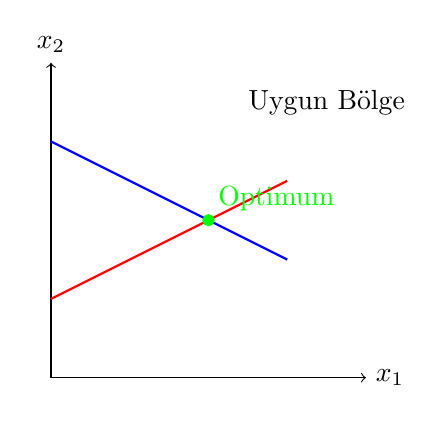
\begin{tikzpicture}
\draw[->] (0,0) -- (4,0) node[right] {$x_1$};
\draw[->] (0,0) -- (0,4) node[above] {$x_2$};
\draw[blue,thick] plot[smooth] coordinates {(0,3) (1,2.5) (2,2) (3,1.5)};
\draw[red,thick] plot[smooth] coordinates {(0,1) (1,1.5) (2,2) (3,2.5)};
\filldraw[green] (2,2) circle (2pt) node[above right] {Optimum};
\node at (3.5,3.5) {Uygun Bölge};
\end{tikzpicture}
\caption{İki kısıtın kesişimi ile oluşan uygun çözüm bölgesi}
\label{fig:feasible_region}
\end{marginfigure}

\subsection{Karar Değişkenleri ve Çözüm Uzayı}

\subsubsection{Karar Değişkenleri}
Karar değişkenleri, optimizasyon sürecinde değerleri belirlenmesi gereken parametrelerdir:
\begin{itemize}
    \item Sürekli (Continuous) değişkenler (örn. boyutlar, kalınlıklar)
    \item Tamsayı (Discrete) değişkenler (örn. eleman sayısı)
    \item İkili (Binary) değişkenler (0-1 kararları)
\end{itemize}

\begin{tcolorbox}[title=Yapısal Tasarımda Karar Değişkenleri]
Bir çelik çerçeve optimizasyonunda:
\begin{itemize}
    \item \textbf{Sürekli:} Kesit boyutları
    \item \textbf{Tamsayı:} Kat sayısı
    \item \textbf{İkili:} Elemanların varlığı/yokluğu
\end{itemize}
\end{tcolorbox}

\subsubsection{Çözüm Uzayı}
Çözüm uzayı, tüm olası karar değişkeni kombinasyonlarının oluşturduğu uzaydır\sidenote{Çözüm uzayının boyutu, karar değişkenlerinin sayısı ile belirlenir. Yüksek boyutlu problemlerde "lanet boyut" (curse of dimensionality) problemi ortaya çıkar.}:
\begin{itemize}
    \item \textbf{Uygun Çözüm Bölgesi:} Tüm kısıtları sağlayan noktalar kümesi
    \item \textbf{Uygun Olmayan Bölge:} En az bir kısıtı ihlal eden noktalar
\end{itemize}


\subsection{Global ve Yerel (Lokal) Minimum/Maksimum Kavramları}

\subsubsection{Yerel Optimum}
Bir nokta, belirli bir komşuluk içinde en iyi değere sahipse yerel optimumdur:
\begin{equation}
x^* \text{ yerel minimum } \Leftrightarrow f(x^*) \leq f(x), \forall x \in N(x^*)
\end{equation}

\subsubsection{Global Optimum}
Tüm çözüm uzayında en iyi değere sahip nokta global optimumdur:
\begin{equation}
x^* \text{ global minimum } \Leftrightarrow f(x^*) \leq f(x), \forall x \in S
\end{equation}

\begin{figure}
\centering
\begin{tikzpicture}
\draw[->] (0,0) -- (7,0) node[right] {$x$};
\draw[->] (0,-1) -- (0,4) node[above] {$f(x)$};
\draw[scale=1,domain=0:7,smooth,variable=\x,blue] plot ({\x},{1 + sin(3*\x r)+sin(\x r)+sin(0.5*\x r)});
\filldraw[gray] (1.526,1.699) circle (2pt) node[below] {Lokal};
\filldraw[gray] (3.774,0.412) circle (2pt) node[below] {Lokal};
\filldraw[black] (5.719,-0.249) circle (2pt) node[below] {Global};
\end{tikzpicture}
\caption{Bir fonksiyonun yerel ve global minimum noktaları}
\label{fig:local_global}
\end{figure}

\subsection{Fiziksel ve Matematiksel Modelleme}

\subsubsection{Fiziksel Modelleme}
Gerçek dünya probleminin fiziksel prensiplere dayalı olarak modellenmesi\sidenote{İyi bir matematiksel model, fiziksel gerçekliği yeterli doğrulukta yansıtmalı, ancak gereksiz karmaşıklıktan kaçınmalıdır. Bu esasen optimizasyonun başlıca konusu olmasa da yapısal optimizasyon açısından oldukça önemli bir konudur.}:
\begin{itemize}
    \item Kuvvet dengesi
    \item Enerji korunumu
    \item Malzeme davranışı
    \item Geometrik ilişkiler
\end{itemize}

\subsubsection{Matematiksel Modelleme}
Fiziksel modelin matematiksel formülasyona dönüştürülmesi:
\begin{itemize}
    \item Diferansiyel denklemler
    \item Cebirsel denklemler
    \item Matris formülasyonları
    \item Sonlu eleman modelleri
\end{itemize}

\subsection{Diferansiyellenebilirlik ve Süreklilik}

\subsubsection{Süreklilik}
Fonksiyonun sürekli olması, küçük girdi değişimlerinin çıktıda ani sıçramalara neden olmaması demektir. Matematiksel olarak:
\begin{equation}
\lim_{x \to x_0} f(x) = f(x_0)
\end{equation}

\begin{tcolorbox}[title=Süreklilik ve Optimizasyon İlişkisi]
Süreklilik, optimizasyon problemlerinde önemli bir özelliktir çünkü:
\begin{itemize}
    \item Sürekli fonksiyonlar için kapalı ve sınırlı bir aralıkta mutlaka bir minimum ve maksimum değer vardır (Weierstrass teoremi).
    \item Sürekli olmayan fonksiyonların optimizasyonu daha zordur çünkü ani sıçramalar, algoritmaların doğru yönde ilerlemesini engelleyebilir.
    \item Gerçek mühendislik problemlerinde çoğu fiziksel davranış, sürekli fonksiyonlarla modellenir (örneğin, bir kirişin yük altında deformasyonu).
\end{itemize}
\end{tcolorbox}

\subsubsection{Diferansiyellenebilirlik}
Fonksiyonun türevinin var olması, fonksiyonun davranışının her noktada bir teğet doğru ile yaklaşık olarak ifade edilebilmesi anlamına gelir. Matematiksel olarak:
\begin{equation}
f'(x_0) = \lim_{h \to 0} \frac{f(x_0 + h) - f(x_0)}{h}
\end{equation}

\begin{tcolorbox}[title=Diferansiyellenebilirlik ve Optimizasyon Arasındaki İlişki]
Diferansiyellenebilirlik, optimizasyon sürecinde kritik bir role sahiptir:
\begin{itemize}
    \item \textbf{Gradyan Bilgisi:} Türev, fonksiyonun en hızlı artış/azalış yönünü verir, böylece optimizasyon algoritmaları nereye gideceklerini bilir.
    \item \textbf{Kritik Noktalar:} Fonksiyonun türevinin sıfır olduğu noktalar (kritik noktalar), potansiyel optimum noktalardır.
    \item \textbf{İkinci Türev:} İkinci türev, kritik noktanın minimum, maksimum veya eğer noktası olduğunu belirlemede yardımcı olur.
\end{itemize}
\end{tcolorbox}

\begin{marginfigure}
    \centering
    \begin{tikzpicture}
    \draw[->] (0,0) -- (6,0) node[right] {$x$};
    \draw[->] (0,0) -- (0,4) node[above] {$f(x)$};
    
    % Fonksiyon
    \draw[blue, thick, domain=0:6, smooth, variable=\x] plot ({\x}, {0.1*\x*\x*\x - 0.9*\x*\x + 2*\x + 0.5});
    
    \end{tikzpicture}
    \caption{Diferansiyellenebilir Fonksiyon ve Gradyan}
    \label{fig:differentiability}
\end{marginfigure}

\begin{marginfigure}
    \centering
    \begin{tikzpicture}
    \draw[->] (0,0) -- (6,0) node[right] {$x$};
    \draw[->] (0,0) -- (0,4) node[above] {$f(x)$};
    
    % Diferansiyellenemeyen fonksiyon (mutlak değer)
    \draw[blue, thick, domain=0:3, smooth, variable=\x] plot ({\x}, {3-\x});
    \draw[blue, thick, domain=3:6, smooth, variable=\x] plot ({\x}, {\x-3});
    
    % Kritik nokta (köşe)
    \filldraw[red] (3,0) circle (2pt) node[below right] {$f'(x)$ tanımsız};
    
    \end{tikzpicture}
    \caption{Diferansiyellenemeyen Fonksiyon (Mutlak Değer Fonksiyonu)}
    \label{fig:non_differentiable}
\end{marginfigure}

\begin{tcolorbox}[title=Gerçek Hayat Örneği: Tepeye Tırmanma]
Düşünün ki bir dağa tırmanıyorsunuz ve hedefiniz zirveye ulaşmak. Eğer sisli bir günde görüş alanınız çok kısıtlıysa, nasıl ilerlemelisiniz?

\begin{itemize}
    \item \textbf{Gradyan (Türev) Bilgisi:} Her adımda ayaklarınızla zeminin eğimini hissederek en dik yokuş yukarı yönünü (negatif gradyan) seçebilirsiniz.
    \item \textbf{Diferansiyellenemeyen Noktalar:} Eğer yolunuz üzerinde dik bir kayalık (türevin tanımlanamadığı nokta) varsa, doğrudan ilerleyemez, farklı bir yol bulmanız gerekir.
    \item \textbf{Yerel Tepe vs. Zirve:} Tırmanışınız sırasında küçük bir tepeye (yerel maksimum) ulaşabilirsiniz, ancak gerçek zirve (global maksimum) başka bir yerde olabilir.
\end{itemize}

Bu anoloji, gradyan tabanlı optimizasyon algoritmalarının çalışma prensibine çok benzerdir.
\end{tcolorbox}


\begin{tcolorbox}[title=Diferansiyellenebilirliğe Göre Optimizasyon Yöntemleri]
\begin{itemize}
    \item \textbf{Diferansiyellenebilir Fonksiyonlar için Gradyan Tabanlı Yöntemler:}
    \begin{itemize}
        \item \textbf{Gradyan İniş:} Fonksiyonun en hızlı düşüş yönünde ilerler.
        \item \textbf{Newton Yöntemi:} İkinci türev bilgisini kullanarak daha hızlı yakınsama sağlar.
        \item \textbf{Quasi-Newton:} İkinci türevi yaklaşık olarak hesaplar (BFGS, L-BFGS gibi).
    \end{itemize}
    
    \item \textbf{Diferansiyellenemeyen Fonksiyonlar için Gradyan-sız Yöntemler:}
    \begin{itemize}
        \item \textbf{Simpleks Arama:} Fonksiyon değerlerini karşılaştırarak en uygun yönü belirler (Nelder-Mead yöntemi).
        \item \textbf{Genetik Algoritmalar:} Evrimsel süreçleri taklit ederek çözüm uzayını araştırır.
        \item \textbf{Parçacık Sürü Optimizasyonu:} Grup davranışını taklit ederek çözüme yaklaşır.
    \end{itemize}
    
    \item \textbf{Karma Problemler için Hibrit Yaklaşımlar:}
    \begin{itemize}
        \item \textbf{Arama + İyileştirme:} Gradyan-sız bir yöntemle geniş bölgede arama, sonra bulduğu noktadan gradyan tabanlı yöntemle iyileştirme.
        \item \textbf{Alt-Gradyan Yöntemleri:} Diferansiyellenemeyen noktalarda bile ilerleme sağlayan genelleştirilmiş türev yaklaşımları.
    \end{itemize}
\end{itemize}
\end{tcolorbox}\sidenote{Yapısal optimizasyon problemleri genellikle diferansiyellenebilir değildir. Bu nedenle, global optimumu bulmak zorlaşır ve metasezgisel yöntemler tercih edilir.}



\subsection{Konveks ve Konveks Olmayan Optimizasyon}

\subsubsection{Konveks Fonksiyonlar}
Bir fonksiyonun konveks olması, fonksiyonun grafiğinin herhangi iki noktasını birleştiren doğru parçasının, bu iki nokta arasındaki fonksiyon grafiğinin üzerinde kalması demektir. Matematiksel olarak, $f: \mathbb{R}^n \rightarrow \mathbb{R}$ fonksiyonu için:
\begin{equation}
f(\lambda x + (1-\lambda)y) \leq \lambda f(x) + (1-\lambda) f(y), \quad \forall x,y \in \mathbb{R}^n, \forall \lambda \in [0,1]
\end{equation}

\begin{figure}[H]
    \centering
    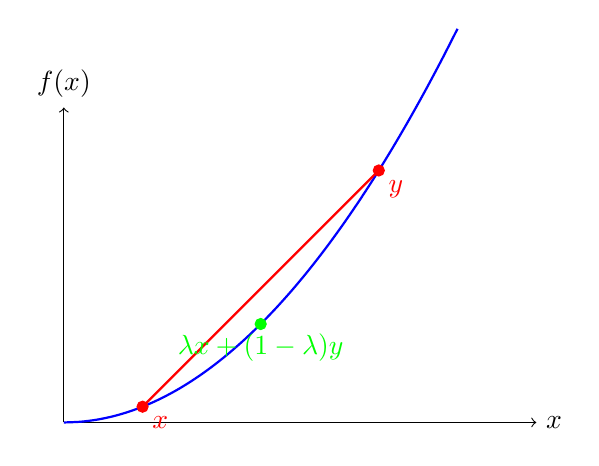
\begin{tikzpicture}
    \draw[->] (0,0) -- (6,0) node[right] {$x$};
    \draw[->] (0,0) -- (0,4) node[above] {$f(x)$};
    
    % Konveks fonksiyon
    \draw[blue, thick, domain=0:5, smooth, variable=\x] plot ({\x}, {0.2*\x*\x});
    
    % İki nokta
    \filldraw[red] (1,0.2) circle (2pt) node[below right] {$x$};
    \filldraw[red] (4,3.2) circle (2pt) node[below right] {$y$};
    
    % Doğru parça
    \draw[red, thick] (1,0.2) -- (4,3.2);
    
    % Orta nokta
    \filldraw[green] (2.5,1.25) circle (2pt) node[below] {$\lambda x + (1-\lambda)y$};
    
    \end{tikzpicture}
    \caption{Konveks Fonksiyon Örneği}
    \label{fig:convex_function}
\end{figure}

\subsubsection{Konveks Küme}
Konveks bir küme, küme içindeki herhangi iki noktayı birleştiren doğru parçasının tamamen küme içinde kalması anlamına gelir:
\begin{equation}
\lambda x + (1-\lambda)y \in S, \quad \forall x,y \in S, \forall \lambda \in [0,1]
\end{equation}

\begin{figure}[H]
    \centering
    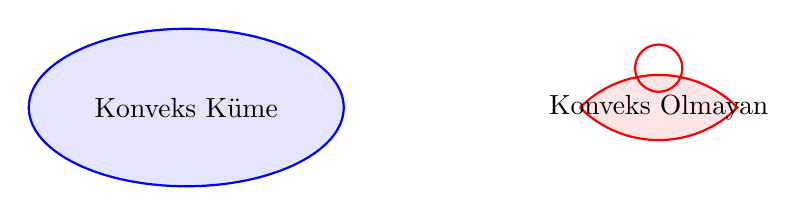
\begin{tikzpicture}
    % Konveks küme
    \draw[blue, thick, fill=blue!10] (0,0) ellipse (2 and 1);
    \node at (0,0) {Konveks Küme};
    
    % Konveks olmayan küme
    \draw[red, thick, fill=red!10] (5,0) to[out=45,in=135] (7,0) to[out=-135,in=-45] (5,0);
    \draw[red, thick] (6,0.5) circle (0.3);
    \node at (6,0) {Konveks Olmayan};
    \end{tikzpicture}
    \caption{Konveks ve Konveks Olmayan Küme Örnekleri}
    \label{fig:convex_nonconvex_sets}
\end{figure}

\subsubsection{Konveks Optimizasyon Avantajları}
Konveks optimizasyon, optimizasyon teorisinde özel bir öneme sahiptir\sidenote{Konveks optimizasyon problemleri için geliştirilmiş etkili algoritmalar ve matematiksel garantiler, bu tür problemlerin çözümünü daha güvenilir hale getirir. Günümüzde sıkça duyduğumuz derin öğrenme algoritmalarının içinde yer alan optimizasyon problemleri genellikle konveks optimizasyon problemleridir. Burada kullanılan optimizasyon algoritmaları genellikle gradyan iniş yöntemleridir. Çok efektif yöntemler olmalarının yanında genellikle yapısaal optimizasyon problemlerinde verimsiz kalırlar. }:

\begin{itemize}
    \item \textbf{Yerel Optimum = Global Optimum:} Konveks bir fonksiyonun yerel minimumu, aynı zamanda global minimumdur. Bu, optimizasyon sürecini önemli ölçüde basitleştirir.
    \item \textbf{Kararlı Çözüm:} Başlangıç noktasından bağımsız olarak, uygun gradyan tabanlı algoritmalar aynı optimum noktaya yakınsar.
    \item \textbf{Verimli Algoritmalar:} İç nokta yöntemleri, gradyan iniş yöntemi gibi algoritmalar konveks problemlerde polinom zamanda çözüme ulaşabilir.
\end{itemize}

\begin{tcolorbox}[title=Konveks Optimizasyon Örneği]
Karesel programlama problemi:
\begin{equation}
\begin{aligned}
\min_{x \in \mathbb{R}^n} & \quad \frac{1}{2}x^TQx + c^Tx \\
\text{s.t.} & \quad Ax \leq b
\end{aligned}
\end{equation}

Eğer $Q$ pozitif yarı-tanımlı bir matris ise, bu problem konvekstir ve verimli iç nokta yöntemleriyle çözülebilir.
\end{tcolorbox}

\subsubsection{Konveks Olmayan Optimizasyon Zorlukları}
Konveks olmayan optimizasyon problemleri, yapısal optimizasyonda sıklıkla karşılaşılan zorluklardır\sidenote{Yapısal optimizasyon problemlerinin çoğu, birden fazla yerel optimum içerebilen konveks olmayan problemlerdir. Bu da global optimumu bulma konusunda güçlükler yaratır.}:

\begin{itemize}
    \item \textbf{Çoklu Yerel Optimumlar:} Fonksiyon birden fazla yerel minimum içerebilir, bu nedenle global optimumu bulmak zorlaşır.
    \item \textbf{Başlangıç Noktası Bağımlılığı:} Gradyan tabanlı algoritmalar, başlangıç noktasına bağlı olarak farklı yerel optimumlara yakınsayabilir.
    \item \textbf{Hesaplama Maliyeti:} Global optimumu bulma garantisi için genellikle daha kapsamlı arama yöntemleri gereklidir, bu da hesaplama maliyetini artırır.
\end{itemize}


\begin{tcolorbox}[title=Konveks Olmayan Problemlere Yaklaşımlar]
\begin{itemize}
    \item \textbf{Çoklu Başlangıç Noktası:} Farklı başlangıç noktalarından birden fazla yerel optimizasyon çalıştırılarak en iyi sonuç seçilir.
    \item \textbf{Metasezgisel Algoritamalar:} Genetik algoritmalar, parçacık sürü optimizasyonu gibi yöntemler, geniş çözüm uzayını araştırarak global optimuma yaklaşmaya çalışır.
    \item \textbf{Konveks Yaklaşımlar:} Problemi konveks alt-problemlere ayrıştırarak veya konveks yaklaşımlar kullanarak çözüm aranabilir (Sequential Convex Programming gibi).
\end{itemize}
\end{tcolorbox}


\subsection{Kısıtsız ve Kısıtlı Optimizasyon}

\subsubsection{Kısıtsız Optimizasyon}
Kısıtsız optimizasyon, adından da anlaşılacağı gibi herhangi bir kısıt içermeyen, sadece amaç fonksiyonunun minimize veya maksimize edilmesi gereken problemleri ifade eder. Matematiksel olarak:
\begin{equation}
\min_{x \in \mathbb{R}^n} f(x)
\end{equation}

\sidenote{Kısıtsız optimizasyon, her ne kadar teorik olarak "kısıtsız" olarak adlandırılsa da, pratikte çoğu mühendislik problemi bir şekilde fiziksel veya matematiksel kısıtlar içerir. Buradaki "kısıtsız" terimi, problemin formülasyonunda açık kısıtlar olmadığı anlamına gelir.}

Kısıtsız optimizasyon problemlerini çözmek için kullanılan başlıca yöntemler \sidenote{Bu beş yöntemin çalışma biçimini test eden python kodu, bağlantı üzerinden test edilebilir. 

\qrcode[height=1in]{https://github.com/btayfur/structural-optimization/blob/main/Code/Examples/Exmp2/}}:

\begin{itemize}
    \item \textbf{Gradyan İniş Yöntemi:} Fonksiyonun en hızlı düşüş yönünde (negatif gradyan yönünde) adım adım ilerleyerek minimuma ulaşmayı hedefler. Bu yöntem, özellikle derin öğrenme ve makine öğrenmesi uygulamalarında yaygın olarak kullanılır.
    
    \item \textbf{Newton Yöntemi:} Fonksiyonun ikinci türev (Hessian) bilgisini de kullanarak, hem yön hem de adım büyüklüğü konusunda daha akıllı kararlar verir. Kuadratik yakınsama özelliği sayesinde, doğru koşullar altında gradyan inişinden daha hızlı yakınsar.
    
    \item \textbf{Quasi-Newton Yöntemleri:} Newton yönteminin hesaplama maliyetini düşürmek için Hessian matrisini doğrudan hesaplamak yerine, yaklaşık olarak tahmin eden yöntemlerdir. BFGS ve L-BFGS en popüler Quasi-Newton algoritmaları arasındadır.
    
    \item \textbf{Eş Gradyan Yöntemi (Conjugate Gradient):} Özellikle büyük ölçekli problemlerde etkili olan ve ardışık arama yönlerinin birbirine "eş" (conjugate) olmasını sağlayan bir yöntemdir.
    
    \item \textbf{Trust Region Yöntemleri:} Her iterasyonda, fonksiyonun yerel olarak iyi modellenebileceği bir "güven bölgesi" belirleyerek bu bölge içinde optimum arayan yöntemlerdir.
\end{itemize}



\begin{tcolorbox}[title=Dağa Tırmanma Analojisi]
Kısıtsız optimizasyon yöntemlerini anlamak için bir dağ tırmanışı analojisi düşünelim (maksimizasyon problemi için):

\begin{itemize}
    \item \textbf{Gradyan Tırmanışı:} Her adımda en dik yokuş yukarı yönde ilerlersiniz. Kolay uygulanır ancak dar vadilerde zigzaglar çizerek yavaş ilerleyebilir.
    
    \item \textbf{Newton Yöntemi:} Sadece zeminin eğimine (gradyan) değil, aynı zamanda arazinin şeklini (Hessian) de bakarsınız. Bu, düz alanlarda büyük adımlar atmanızı, dik yamaçlarda küçük ve dikkatli adımlar atmanızı sağlar.
    
    \item \textbf{Quasi-Newton:} Arazinin şeklini tam ölçmek yerine, önceki adımlarınızdan tahmin edersiniz. Bu, Newton kadar etkili olmasa da çok daha az çaba gerektirir.
\end{itemize}
\end{tcolorbox}

\subsubsection{Kısıtlı Optimizasyon}
Kısıtlı optimizasyon, gerçek dünya problemlerinin modellenmesinde çok daha yaygındır ve amaç fonksiyonunun yanı sıra bir dizi kısıt içerir. Bu kısıtlar, çözümün sağlaması gereken şartları temsil eder. Matematiksel formülasyonu:
\begin{equation}
\begin{aligned}
\min_{x \in \mathbb{R}^n} & \quad f(x) \\
\text{s.t.} & \quad g_i(x) \leq 0, \quad i = 1,\ldots,m \\
& \quad h_j(x) = 0, \quad j = 1,\ldots,p
\end{aligned}
\end{equation}

Burada $g_i(x) \leq 0$ eşitsizlik kısıtlarını, $h_j(x) = 0$ ise eşitlik kısıtlarını temsil eder.

\sidenote{Yapısal optimizasyon problemleri neredeyse her zaman kısıtlı problemlerdir. Bir köprünün ağırlığını minimize etmek istediğinizde, köprünün belirli yükleri taşıyabilmesi, belirli bir güvenlik faktörüne sahip olması ve inşa edilebilir olması gibi çeşitli kısıtlar vardır. Bu kısıtlar olmadan yapılan bir optimizasyon, pratikte uygulama alanı bulamaz.}

Kısıtlı optimizasyon problemlerini çözmek için kullanılan başlıca yöntemler:

\begin{itemize}
    \item \textbf{Lagrange Çarpanları Yöntemi:} Eşitlik kısıtlı problemler için Lagrange çarpanları adı verilen ek değişkenler tanımlayarak, kısıtlı problemi genişletilmiş bir kısıtsız probleme dönüştürür. Bu yöntem, kısıtların tam olarak sağlanması gerektiği durumlarda özellikle kullanışlıdır.
    
    \item \textbf{Karush-Kuhn-Tucker (KKT) Koşulları:} Hem eşitlik hem de eşitsizlik kısıtları için geçerli olan optimalite koşullarıdır. KKT koşulları, Lagrange çarpanları yönteminin eşitsizlik kısıtlarına genelleştirilmiş halidir.
    
    \item \textbf{Ceza Fonksiyonu Yöntemleri:} Kısıtlı problemi, kısıtların ihlaline ceza vererek kısıtsız bir probleme dönüştürür. İki ana yaklaşım vardır:
    \begin{itemize}
        \item \textbf{Dış Ceza (Penalty) Metodu:} Kısıt ihlalleri için ceza ekler, uygun olmayan çözümlere izin verir ancak cezalandırır.
        \item \textbf{İç Ceza (Barrier) Metodu:} Fizibil bölgenin sınırına yaklaşıldıkça giderek artan bir ceza ekler, böylece çözümün fizibil bölgenin içinde kalmasını sağlar.
    \end{itemize}
    
    \item \textbf{Aktif Set Yöntemleri:} Her iterasyonda, aktif olduğu düşünülen kısıtları belirleyerek daha küçük bir alt problem çözer. Bu, özellikle doğrusal ve kuadratik programlama problemlerinde etkilidir.
    
    \item \textbf{İç Nokta (Interior Point) Yöntemleri:} Fizibil bölgenin içinde kalarak optimuma yaklaşır. Bariyer fonksiyonları kullanır ama kısıtları doğrudan ele alır. Büyük ölçekli doğrusal ve konveks programlama problemlerinde çok etkilidir.
    
    \item \textbf{Ardışık Karesel Programlama (SQP):} Kısıtlı doğrusal olmayan problemleri, bir dizi karesel alt probleme dönüştürerek çözer. Yapısal optimizasyonda yaygın olarak kullanılır.
\end{itemize}

\begin{tcolorbox}[title=Kısıtlı Optimizasyon Analojisi: Patika Bulma]
Kısıtlı optimizasyonu, hedefinize giden en iyi yolu bulmaya çalışırken belirli kurallara uymak zorunda olduğunuz bir patika bulma problemi olarak düşünebilirsiniz:

\begin{itemize}
    \item \textbf{Hedefiniz (Amaç Fonksiyonu):} Dağın zirvesine ulaşmak.
    \item \textbf{Kısıtlarınız:} Sadece işaretli patikalardan yürüyebilirsiniz (eşitlik kısıtları), bazı tehlikeli bölgelerden uzak durmalısınız (eşitsizlik kısıtları).
    
    \item \textbf{Lagrange Yöntemi:} Patika haritasını ve tehlikeli bölgeleri sürekli kontrol ederek ilerlemeye benzer.
    
    \item \textbf{Ceza Metodu:} İşaretli patikadan çıkarsanız, ekstra zorluk yaşarsınız (çamura saplanma, dikenli çalılıklardan geçme gibi). Bu cezalara rağmen bazen kestirme yapmak avantajlı olabilir.
    
    \item \textbf{Bariyer Metodu:} Tehlikeli bölgelerin etrafında görünmez bir "itici güç" varmış gibi davranırsınız, yaklaştıkça geri çekilirsiniz. Böylece her zaman güvenli bölgede kalırsınız.
\end{itemize}
\end{tcolorbox}

\begin{tcolorbox}[title=Kısıtların Ele Alınması]
Kısıtlı bir problemi kısıtsız probleme dönüştürme yöntemleri:

\begin{itemize}
    \item \textbf{Dış Ceza (Penalty) Yöntemi:} 
    \begin{equation}
    \min f(x) + c\sum\max(0,g_i(x))^2 + c\sum(h_j(x))^2
    \end{equation}
    
    Burada $c > 0$ ceza parametresidir ve genellikle iterasyonlar boyunca artırılır. Kısıt ihlalleri arttıkça ceza da artar, böylece algoritma zamanla fizibil bölgeye doğru yönlendirilir.
    
    \item \textbf{İç Ceza (Barrier) Yöntemi:} 
    \begin{equation}
    \min f(x) - c\sum\ln(-g_i(x))
    \end{equation}
    
    Bu yöntem, sadece $g_i(x) < 0$ (yani fizibil bölge içinde) olduğunda tanımlıdır ve kısıt sınırına yaklaştıkça $\ln(-g_i(x)) \to -\infty$ olur, bu da çözümün fizibil bölge içinde kalmasını sağlar. $c$ parametresi genellikle iterasyonlar boyunca azaltılır.
    
    \item \textbf{Augmented Lagrangian Yöntemi:} 
    \begin{equation}
    \min f(x) + \sum\lambda_j h_j(x) + \frac{c}{2}\sum(h_j(x))^2 + \sum\mu_i\max(0,g_i(x)) + \frac{c}{2}\sum\max(0,g_i(x))^2
    \end{equation}
    
    Bu yöntem, Lagrange çarpanları ve ceza yöntemlerinin avantajlarını birleştirir. Lagrange çarpanları $\lambda_j$ ve $\mu_i$ her iterasyonda güncellenir.
\end{itemize}
\end{tcolorbox}

\subsubsection{Kısıtlı ve Kısıtsız Optimizasyonun Karşılaştırılması}

\begin{itemize}
    \item \textbf{Problem Zorluğu:} Kısıtlı problemler genellikle daha zordur ve daha özel çözüm yöntemleri gerektirir.
    
    \item \textbf{Çözüm Uzayı:} Kısıtsız problemlerde tüm arama uzayı kullanılabilirken, kısıtlı problemlerde arama "fizibil bölge" ile sınırlıdır.
    
    \item \textbf{Gerçekçilik:} Gerçek mühendislik problemleri neredeyse her zaman kısıtlıdır, çünkü tasarımların belirli gereksinimleri karşılaması gerekir.
    
    \item \textbf{Çözüm Stratejisi:} Kısıtlı problemlerin çözümünde, genellikle önce kısıtların sağlanması, sonra amaç fonksiyonunun optimize edilmesi hedeflenir, ya da bu iki hedef dengeli bir şekilde ele alınır.
\end{itemize}

\sidenote{Yapısal optimizasyon problemleri genellikle oldukça karmaşık kısıtlar içerir. Örneğin, bir gökdelenin tasarımında, maliyeti minimize ederken yapı dayanımı, kullanıcı konforu, deprem performansı, rüzgar yükleri gibi çok sayıda faktör kısıt olarak dikkate alınır. Bu kısıtların doğrusal olmaması ve birbiriyle etkileşimi, problemi çözmek için özel tekniklerin geliştirilmesini gerektirir.}

\subsection{Optimizasyon Yaklaşımlarının Sınıflandırılması}

\subsubsection{Problem Yapısına Göre}
Optimizasyon problemleri, matematiksel yapılarına göre çeşitli kategorilere ayrılabilir, bu sınıflandırma hangi çözüm yöntemlerinin uygun olacağını belirlememize yardımcı olur:

\begin{itemize}
    \item \textbf{Doğrusal Programlama (Linear Programming - LP)}
        \begin{itemize}
            \item Doğrusal amaç fonksiyonu: $f(x) = c^T x$
            \item Doğrusal kısıtlar: $Ax \leq b$, $Aeq \cdot x = beq$
            \item Temel çözüm yöntemi: Simpleks algoritması, İç nokta yöntemleri
            \item Özellikler: Tek bir global optimum, kısıtlar tarafından tanımlanan konveks bir fizibil bölge
            \item Uygulama alanları: Kaynak tahsisi, üretim planlama, lojistik optimizasyonu
        \end{itemize}
        
    \item \textbf{Doğrusal Olmayan Programlama (Nonlinear Programming - NLP)}
        \begin{itemize}
            \item Doğrusal olmayan amaç fonksiyonu ve/veya kısıtlar
            \item Alt kategori - Konveks Programlama: Amaç fonksiyonu konveks, kısıt kümesi konveks
            \item Alt kategori - Konveks Olmayan Programlama: Amaç fonksiyonu ve/veya kısıt kümesi konveks değil
            \item Çözüm yöntemleri: Gradyan tabanlı yöntemler (SQP, İç nokta, BFGS), metasezgisel yöntemler
            \item Uygulama alanları: Yapısal tasarım, mekanik sistemlerin optimizasyonu, ekonomik modeller
        \end{itemize}
        
    \item \textbf{Tamsayılı Programlama (Integer Programming - IP)}
        \begin{itemize}
            \item Tüm değişkenler tamsayı olmalıdır: $x \in \mathbb{Z}^n$
            \item Alt kategori - Karma Tamsayılı Programlama (MIP): Bazı değişkenler tamsayı, bazıları sürekli
            \item Alt kategori - 0-1 Tamsayılı Programlama: Değişkenler yalnızca 0 veya 1 değerini alabilir
            \item Çözüm yöntemleri: Dal-sınır (Branch-and-bound), kesme düzlemi (Cutting plane), dal-kesme (Branch-and-cut)
            \item Uygulama alanları: Çizelgeleme problemleri, kesme/paketleme problemleri, topoloji optimizasyonu
        \end{itemize}
        
    \item \textbf{Stokastik Programlama}
        \begin{itemize}
            \item Rastgele değişkenler içeren problemler
            \item Belirsizliğin olasılık dağılımları ile modellendiği durumlar
            \item Çözüm yöntemleri: Senaryo yaklaşımı, örnek ortalamalı yaklaşım, robust optimizasyon
            \item Uygulama alanları: Risk yönetimi, portföy optimizasyonu, belirsizlik altında yapısal tasarım
        \end{itemize}
        
    \item \textbf{Çok Amaçlı Programlama}
        \begin{itemize}
            \item Birden fazla amaç fonksiyonunun eş zamanlı optimize edilmesi
            \item Çözüm kavramı: Pareto-optimal çözüm kümesi
            \item Çözüm yöntemleri: Ağırlıklı toplam yöntemi, epsilon-kısıt yöntemi, NSGA-II gibi evrimsel algoritmalar
            \item Uygulama alanları: Mühendislik tasarımı, çevre yönetimi, ekonomik modeller
        \end{itemize}
\end{itemize}

\sidenote{Bir yapısal optimizasyon problemi, genellikle yukarıdaki kategorilerin birkaçının özelliklerini bir arada taşır. Örneğin, bir köprü tasarımında kesit boyutları sürekli değişkenler olabilirken, kullanılacak eleman tipleri tamsayı değişkenler olabilir. Ayrıca malzeme davranışı doğrusal olmayan denklemlerle ifade edilebilir, ve hem maliyet hem de deplasman gibi birden fazla kriteri optimize etmek gerekebilir. Bu durumda problem, karma tamsayılı, doğrusal olmayan, çok amaçlı bir optimizasyon problemi olur.}

\subsubsection{Çözüm Stratejisine Göre}
Optimizasyon problemlerini çözmek için kullanılan algoritmalar, arama stratejilerine göre kategorize edilebilir:

\begin{itemize}
    \item \textbf{Deterministik Yöntemler}
        \begin{itemize}
            \item \textbf{Gradyan tabanlı yöntemler:} Fonksiyonun türev bilgisini kullanarak en hızlı iyileşme yönünde ilerler.
                \begin{itemize}
                    \item Avantajları: Genellikle hızlı yakınsama, yerel optimuma kesin ulaşma
                    \item Dezavantajları: Yerel optimumlara takılma, türev hesaplama gereksinimi
                    \item Örnekler: Gradyan iniş, Newton, BFGS, Conjugate gradient
                \end{itemize}
                
            \item \textbf{Doğrudan arama yöntemleri:} Türev bilgisi kullanmadan, fonksiyon değerlendirmeleri ile ilerler.
                \begin{itemize}
                    \item Avantajları: Türev gerektirmez, gürültülü fonksiyonlar için uygun
                    \item Dezavantajları: Genellikle daha yavaş yakınsama
                    \item Örnekler: Nelder-Mead simpleks, Hooke-Jeeves pattern search
                \end{itemize}
                
            \item \textbf{İç nokta yöntemleri:} Fizibil bölgenin içinde kalarak optimuma ulaşır.
                \begin{itemize}
                    \item Avantajları: Büyük ölçekli problemlerde etkili, polinom zamanlı algoritma
                    \item Dezavantajları: Karmaşık implementasyon, başlangıç noktası gereksinimi
                    \item Örnekler: Primal-dual iç nokta, bariyer yöntemleri
                \end{itemize}
        \end{itemize}
    
    \item \textbf{Stokastik/Metasezgisel Yöntemler}
        \begin{itemize}
            \item \textbf{Evrimsel algoritmalar:} Doğal seleksiyon ve genetik mekanizmaları taklit eder.
                \begin{itemize}
                    \item Avantajları: Global optimumu bulma potansiyeli, türev gerektirmez, paralel işleme uygun
                    \item Dezavantajları: Hesaplama maliyeti yüksek, parametre ayarı hassas
                    \item Örnekler: Genetik algoritmalar, diferansiyel evrim, evrim stratejileri
                \end{itemize}
                
            \item \textbf{Sürü tabanlı algoritmalar:} Hayvan gruplarının kolektif davranışlarını modelleyerek çözüm arar.
                \begin{itemize}
                    \item Avantajları: Kolay implementasyon, konveks olmayan problemlerde etkili
                    \item Dezavantajları: Teorik garantiler zayıf, çözüm kalitesi değişken
                    \item Örnekler: Parçacık sürü optimizasyonu, karınca kolonisi optimizasyonu, arı algoritması
                \end{itemize}
                
            \item \textbf{Fizik tabanlı algoritmalar:} Fiziksel süreçleri taklit ederek optimizasyon yapar.
                \begin{itemize}
                    \item Avantajları: Yerel optimumlardan kaçabilme yeteneği
                    \item Dezavantajları: Yavaş yakınsama, parametre hassasiyeti
                    \item Örnekler: Tavlama benzetimi, harmony search, big bang-big crunch
                \end{itemize}
        \end{itemize}
    
    \item \textbf{Hibrit Yöntemler} \sidenote{Hibrit yöntemler, farklı yaklaşımların avantajlarını birleştirerek daha gürbüz ve etkili çözümler sunar. Örneğin, global arama için bir genetik algoritma ile başlayıp, bulunan umut verici bölgeleri yerel bir gradyan tabanlı algoritma ile iyileştirmek, hem global optimumu bulma şansını artırır hem de hassas bir çözüme ulaşmayı sağlar.}
        \begin{itemize}
            \item \textbf{Deterministik + Stokastik hibrit:} İki yaklaşımın avantajlarını birleştirir.
                \begin{itemize}
                    \item Avantajları: Global aramayı yerel optimizasyon ile birleştirme
                    \item Dezavantajları: Karmaşık implementasyon, parametre ayarı zorluğu
                    \item Örnekler: Memetic algoritmalar, çoklu başlangıç noktalı gradyan yöntemleri
                \end{itemize}
                
            \item \textbf{Çok seviyeli yaklaşımlar:} Problemi farklı detay seviyelerinde ele alır.
                \begin{itemize}
                    \item Avantajları: Büyük ve karmaşık problemleri çözebilme yeteneği
                    \item Dezavantajları: Problem yapısına özgü tasarım gereksinimi
                    \item Örnekler: Kaba-ince (coarse-fine) grid yöntemleri, hiyerarşik optimizasyon
                \end{itemize}
                
            \item \textbf{Adaptif stratejiler:} Optimizasyon süreci boyunca algoritma parametrelerini veya stratejileri değiştirir.
                \begin{itemize}
                    \item Avantajları: Problem özelliklerine dinamik adaptasyon
                    \item Dezavantajları: Karmaşık kontrol mekanizmaları
                    \item Örnekler: Adaptif metasezgisel yöntemler, self-adaptive evrim stratejileri \sidenote{Yapısal optimizasyon problemlerinde, sonlu eleman analizinin hesaplama maliyeti genellikle yüksek olduğundan, mümkün olduğunca az fonksiyon değerlendirmesi yapan algoritmalar tercih edilir. Bu nedenle, surrogate model tabanlı optimizasyon yöntemleri giderek popülerlik kazanmaktadır. Bu yöntemler, gerçek analiz yerine daha hızlı hesaplanabilen yaklaşık modeller kullanarak optimizasyon sürecini hızlandırır.} 
                \end{itemize}
        \end{itemize}
\end{itemize} 

\begin{tcolorbox}[title=Optimizasyon Algoritması Seçimi]
Bir optimizasyon problemi için hangi algoritmanın en uygun olduğu, problemin özelliklerine bağlıdır:

\begin{itemize}
    \item \textbf{Problem boyutu:} Büyük ölçekli problemler için İç nokta yöntemleri, gradyan tabanlı yöntemler veya özel tasarlanmış metasezgisel yöntemler uygundur.
    
    \item \textbf{Türev bilgisi:} Türev hesaplaması mümkün ve ekonomikse, gradyan tabanlı yöntemler genellikle daha hızlıdır. Türev hesaplaması zor veya imkansızsa, doğrudan arama veya metasezgisel yöntemler tercih edilir.
    
    \item \textbf{Problemin doğası:} Konveks problemler için deterministik yöntemler genellikle yeterlidir. Konveks olmayan, multimodal problemler için metasezgisel veya hibrit yöntemler daha uygundur.
    
    \item \textbf{Hesaplama bütçesi:} Sınırlı hesaplama kaynakları varsa, daha verimli deterministik yöntemler tercih edilebilir. Yüksek hesaplama gücü mevcutsa, daha kapsamlı global arama yöntemleri kullanılabilir.
    
    \item \textbf{Fizibil çözüm önemi:} Eğer ara iterasyonlarda da fizibil çözümler gerekiyorsa, fizibil bölge içinde kalan yöntemler (iç nokta, bariyer yöntemleri) tercih edilebilir.
\end{itemize}
\end{tcolorbox}

  
\section{Klasik Optimizasyon Algoritmalarının Teorik Temelleri}

Geleneksel optimizasyon yöntemleri, modern algoritmaların temel prensiplerini oluşturmakla kalmaz, aynı zamanda mühendislik problemlerinin çözümünde hala başvurulan en güvenilir araçlar arasındadır. Bu bölümde, bu yöntemlerin matematiksel altyapısına derinlemesine bir bakış sunacak ve yapısal optimizasyon problemlerine nasıl uygulandığını inceleyeceğiz.

\subsection{Matematiksel Optimizasyonun Analitik Temelleri}

Optimizasyon, matematik tarihi boyunca en köklü problemlerden biri olmuştur. Leibniz ve Newton'un diferansiyel hesabı geliştirmesinden önce bile matematikçiler optimizasyon problemleriyle uğraşmaktaydı. Modern anlamda matematiksel optimizasyonun analitik temelleri üç temel kavrama dayanır: stasyonerlik (durağanlık), konvekslik ve dualite.

\begin{tcolorbox}[title=Tarihsel Perspektif]
\begin{itemize}
    \item \textbf{Eski Yunan:} Öklidyen geometri ve maksimum-minimum problemleri
    \item \textbf{17. Yüzyıl:} Fermat, Leibniz ve Newton'un diferansiyel hesabı
    \item \textbf{18. Yüzyıl:} Lagrange ve Euler'in varyasyonel hesaplamaları
    \item \textbf{19. Yüzyıl:} Hamilton ve Jacobi'nin optimizasyon teorileri
    \item \textbf{20. Yüzyıl:} Doğrusal programlama, sayısal optimizasyon ve karmaşık algoritmaların gelişimi
\end{itemize}
\end{tcolorbox}

\subsubsection{Birinci ve İkinci Dereceden İyileştirme Koşulları}

Optimizasyonun matematiksel temelini oluşturan en önemli analitik koşullar şunlardır:

\textbf{Birinci Dereceden Gerek Koşul (Stasyonerlik):} 
Eğer $x^*$ noktası bir yerel minimum ise, $\nabla f(x^*) = 0$ olmalıdır. Bu, fonksiyonun gradyanının sıfır olduğu, yani teğet düzlemin yatay olduğu anlamına gelir.

\textbf{İkinci Dereceden Yeter Koşul:} 
Eğer $\nabla f(x^*) = 0$ ve Hessian matrisi $\nabla^2 f(x^*)$ pozitif tanımlı ise, $x^*$ bir kesin yerel minimumdur. Matematiksel olarak, tüm $d \neq 0$ için $d^T \nabla^2 f(x^*) d > 0$ koşulunun sağlanması gerekir.


\sidenote{İkinci dereceden koşullar, kritik noktanın (gradyanın sıfır olduğu nokta) yerel minimum, yerel maksimum veya eğer noktası olduğunu belirlememize yardımcı olur. Yapısal optimizasyon problemlerinde Hessian matrisinin değerlendirilmesi, algoritmanın ilerleyişi için kritik öneme sahiptir.}

\subsubsection{Konveks Optimizasyon Özel Durumu}

Konveks optimizasyon, klasik optimizasyon teorisinin özel bir durumudur ve dikkate değer özellikler taşır:

\begin{itemize}
    \item Amaç fonksiyonu ve kısıt kümesi konveks ise, her yerel minimum aynı zamanda global minimumdur
    \item Konveks problemlerde kritik nokta koşulları, global optimumu garanti eder
    \item Yapısal mekanikte doğrusal elastik yapıslar için potansiyel enerji minimizasyonu konveks bir problemdir
    \item Konveks olmayan problemler için bile, problem sıklıkla konveks alt problemlere ayrıştırılabilir
\end{itemize}

\begin{marginfigure}
\centering
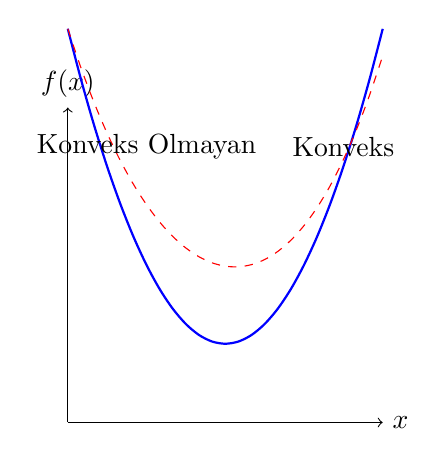
\begin{tikzpicture}
\draw[->] (0,0) -- (4,0) node[right] {$x$};
\draw[->] (0,0) -- (0,4) node[above] {$f(x)$};

% Konveks ve konveks olmayan fonksiyonlar
\draw[scale=1,domain=0:4,smooth,variable=\x,blue,thick] plot ({\x},{(\x-2)^2+1});
\node at (3.5,3.5) {Konveks};

\draw[scale=1,domain=0:4,smooth,variable=\x,red,dashed] plot ({\x},{sin(50*\x)+(\x-2)^2+1});
\node at (1,3.5) {Konveks Olmayan};

\end{tikzpicture}
\caption{Konveks ve konveks olmayan fonksiyonların karşılaştırması}
\label{fig:convexity}
\end{marginfigure}

\subsection{Gradyan Tabanlı Optimizasyon Algoritmaları}

Gradyan tabanlı algoritmalar, fonksiyonun türev bilgisini kullanarak sistematik bir şekilde optimum noktaya yaklaşan yöntemlerdir. Bu yöntemler, hesaplama verimliliği ve yakınsama özellikleri açısından yapısal optimizasyon problemlerinde büyük önem taşır.

\subsubsection{Gradyan İniş Yöntemi ve Varyasyonları}
Gradyan iniş yöntemi, en temel ve en eski gradyan tabanlı optimizasyon yöntemidir. Bu yöntem, fonksiyonun en hızlı azaldığı yönde ilerleyerek minimum noktaya ulaşmayı amaçlar.

\begin{equation}
x_{k+1} = x_k - \alpha_k \nabla f(x_k)
\end{equation}

Burada $\alpha_k$, adım boyutunu (veya öğrenme oranını) temsil eder ve algoritmanın performansını büyük ölçüde etkiler.

\begin{tcolorbox}[title=Gradyan İniş Varyasyonları]
\begin{itemize}
    \item \textbf{Sabit Adım Boyutu:} En basit yaklaşım, tüm iterasyonlarda sabit $\alpha$ kullanmaktır. Ancak hızlı yakınsama için çok düşük, stabilite için çok yüksek olabilir.
    
    \item \textbf{Line Search:} Her iterasyonda, $f(x_k - \alpha \nabla f(x_k))$ ifadesini minimize eden $\alpha_k$ değeri bulunur. Bu yaklaşım, Armijo, Wolfe veya Goldstein koşulları ile uygulanabilir.
    
    \item \textbf{Momentumlu Gradyan İniş:} Önceki gradyan değerlerini de dikkate alarak, yerel minimumlara takılmayı azaltır:
    $$x_{k+1} = x_k - \alpha_k \nabla f(x_k) + \beta (x_k - x_{k-1})$$
    
    \item \textbf{Nesterov Hızlandırılmış Gradyan:} Momentumlu gradyan inişin geliştirilmiş halidir, gradyanı mevcut konumda değil, momentumun götüreceği noktada hesaplar.
\end{itemize}
\end{tcolorbox}

\sidenote{Yapısal optimizasyon problemlerinde, gradyan iniş yöntemi genellikle büyük ölçekli problemlerin ilk aşamalarında kullanılır. Yakınsama hızı düşük olsa da, hesaplama maliyeti düşüktür ve karmaşık problemlerde iyi bir başlangıç noktası sağlayabilir.}

\begin{marginfigure}
\centering
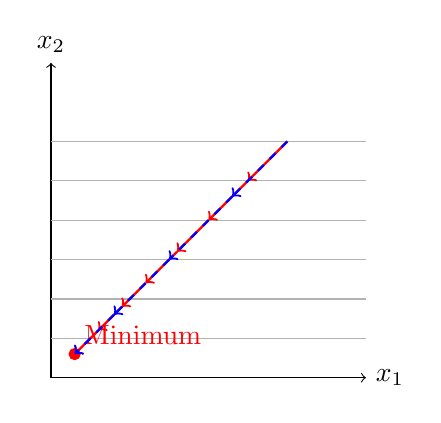
\begin{tikzpicture}
\draw[->] (0,0) -- (4,0) node[right] {$x_1$};
\draw[->] (0,0) -- (0,4) node[above] {$x_2$};

% Kontur çizgileri
\draw[scale=1,domain=0:4,smooth,variable=\x,black!30,thin] plot ({\x},{0.5});
\draw[scale=1,domain=0:4,smooth,variable=\x,black!30,thin] plot ({\x},{1.0});
\draw[scale=1,domain=0:4,smooth,variable=\x,black!30,thin] plot ({\x},{1.5});
\draw[scale=1,domain=0:4,smooth,variable=\x,black!30,thin] plot ({\x},{2.0});
\draw[scale=1,domain=0:4,smooth,variable=\x,black!30,thin] plot ({\x},{2.5});
\draw[scale=1,domain=0:4,smooth,variable=\x,black!30,thin] plot ({\x},{3.0});

% Gradyan iniş yolu
\draw[->,red,thick] (3,3) -- (2.5,2.5);
\draw[->,red,thick] (2.5,2.5) -- (2.0,2.0);
\draw[->,red,thick] (2.0,2.0) -- (1.6,1.6);
\draw[->,red,thick] (1.6,1.6) -- (1.2,1.2);
\draw[->,red,thick] (1.2,1.2) -- (0.9,0.9);
\draw[->,red,thick] (0.9,0.9) -- (0.6,0.6);
\draw[->,red,thick] (0.6,0.6) -- (0.3,0.3);
\filldraw[red] (0.3,0.3) circle (2pt) node[above right] {Minimum};

% Momentumlu gradyan iniş yolu
\draw[->,blue,thick,dashed] (3,3) -- (2.3,2.3);
\draw[->,blue,thick,dashed] (2.3,2.3) -- (1.5,1.5);
\draw[->,blue,thick,dashed] (1.5,1.5) -- (0.8,0.8);
\draw[->,blue,thick,dashed] (0.8,0.8) -- (0.3,0.3);

\end{tikzpicture}
\caption{Gradyan iniş (kırmızı, düz) ve momentumlu gradyan iniş (mavi, kesikli) yöntemlerinin karşılaştırması}
\label{fig:gradient_descent_variants}
\end{marginfigure}

\paragraph{Yapısal Optimizasyonda Gradyan Hesaplama}
Yapısal optimizasyon problemlerinde, gradyan hesaplama için genellikle üç yöntem kullanılır:

\begin{itemize}
    \item \textbf{Analitik Gradyan:} Doğrudan diferansiyel hesaplama ile elde edilir. En doğru sonucu verir ancak karmaşık sistemlerde türev çıkarımı zor olabilir.
    
    \item \textbf{Sonlu Farklar:} Sayısal yaklaşımla gradyan hesaplanır:
    $$\frac{\partial f}{\partial x_i} \approx \frac{f(x + h e_i) - f(x)}{h}$$
    Hesaplaması kolaydır ancak $h$ değerinin seçimi hassastır ve büyük sistemlerde hesaplama maliyeti yüksektir.
    
    \item \textbf{Adjoint Yöntemi:} Özellikle büyük ölçekli yapısal problemlerde verimlidir. Tasarım değişkeni sayısından bağımsız olarak sabit sayıda sistem çözümü gerektirir. Sonlu eleman analizlerinde sıklıkla kullanılır.
\end{itemize}

\subsubsection{Newton ve Quasi-Newton Yöntemleri}
Newton yöntemi, klasik optimizasyonun en güçlü araçlarından biridir. İkinci dereceden türev bilgisini (Hessian matrisini) kullanarak, fonksiyonun yerel kuadratik yaklaşımını oluşturur ve bu yaklaşımın minimum noktasına doğrudan ilerler.

\begin{equation}
x_{k+1} = x_k - [\nabla^2 f(x_k)]^{-1} \nabla f(x_k)
\end{equation}

Newton yönteminin en büyük avantajı, kuadratik yakınsama hızıdır; yani, optimum noktaya yaklaştıkça, hata her iterasyonda yaklaşık olarak karesi kadar azalır. Ancak, Hessian matrisinin hesaplanması ve tersinin alınması, özellikle yüksek boyutlu problemlerde hesaplama açısından maliyetlidir.

\paragraph{Modifiye Newton Yöntemleri}
Hesaplama maliyetini azaltmak ve Newton yönteminin kararsız olabileceği durumlarda daha iyi performans elde etmek için çeşitli modifikasyonlar geliştirilmiştir:

\begin{itemize}
    \item \textbf{Levenberg-Marquardt Algoritması:} Hessian matrisini, daha kararlı hale getirmek için modifiye eder:
    $$x_{k+1} = x_k - [\nabla^2 f(x_k) + \lambda I]^{-1} \nabla f(x_k)$$
    Burada $\lambda$, algoritmanın davranışını ayarlayan bir damping parametresidir.
    
    \item \textbf{Trust Region Newton Metodu:} Her iterasyonda, Hessian matrisinin geçerli olduğu bir "güvenilir bölge" tanımlar ve bu bölge içinde kuadratik modeli minimize eder. Özellikle yapısal optimizasyonda yaygın kullanılır.
\end{itemize}

\paragraph{Quasi-Newton Yöntemleri}
Tam Hessian matrisini hesaplama maliyetini ortadan kaldırmak için, quasi-Newton yöntemleri, Hessian matrisinin yaklaşık bir değerini iteratif olarak günceller. En popüler quasi-Newton yöntemleri şunlardır:

\begin{equation}
x_{k+1} = x_k - B_k^{-1} \nabla f(x_k)
\end{equation}

Burada $B_k$, Hessian matrisinin $k$. iterasyondaki yaklaşımıdır.

\begin{tcolorbox}[title=Temel Quasi-Newton Algoritmaları]
\begin{itemize}
    \item \textbf{BFGS (Broyden-Fletcher-Goldfarb-Shanno):} En yaygın kullanılan quasi-Newton yöntemidir. Hessian yaklaşımının pozitif tanımlılığını korur, bu da algoritmanın kararlılığını artırır. Yapısal optimizasyon problemlerinde sıklıkla tercih edilir.
    
    \item \textbf{DFP (Davidon-Fletcher-Powell):} BFGS'den daha eski bir yöntemdir, ancak genellikle BFGS kadar kararlı değildir.
    
    \item \textbf{SR1 (Symmetric Rank-One):} Daha az hesaplama gerektirir ancak pozitif tanımlılığı garanti etmez.
    
    \item \textbf{L-BFGS (Limited-memory BFGS):} Çok yüksek boyutlu problemler için geliştirilmiş, bellek kullanımı optimize edilmiş BFGS versiyonudur. Büyük ölçekli yapısal optimizasyon problemlerinde, özellikle topoloji optimizasyonunda tercih edilir.
\end{itemize}
\end{tcolorbox}

\paragraph{Yapısal Optimizasyonda Newton ve Quasi-Newton Uygulamaları}
Yapısal mühendislikte, Newton ve quasi-Newton yöntemleri şu tür problemlerde sıklıkla kullanılır:

\begin{itemize}
    \item \textbf{Şekil Optimizasyonu:} Yapının dış geometrisinin optimize edilmesinde, özellikle aerodinamik performans veya termal davranış için
    
    \item \textbf{Kesit Optimizasyonu:} Kafes ve çerçeve yapıların eleman kesitlerinin optimizasyonunda, özellikle doğrusal olmayan davranış gösteren yapılarda
    
    \item \textbf{Parametre Kalibrasyonu:} Sonlu eleman modellerinin deneysel verilerle kalibrasyonunda, malzeme parametrelerinin belirlenmesinde
    
    \item \textbf{Multi-fizik Optimizasyon:} Yapısal, termal ve akışkan davranışların birlikte optimize edildiği karmaşık mühendislik problemlerinde
\end{itemize}

\begin{marginfigure}
\centering
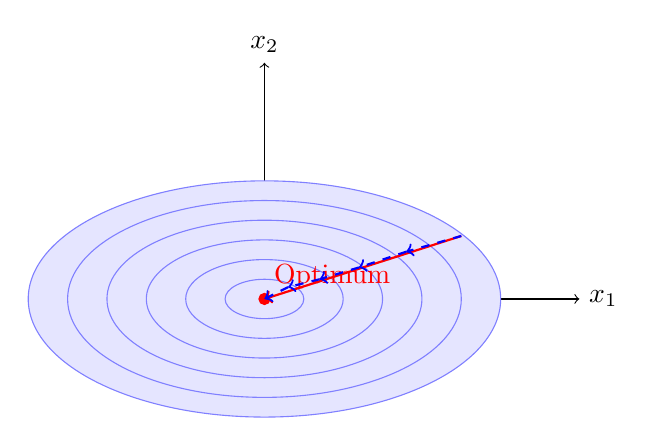
\begin{tikzpicture}
\draw[->] (0,0) -- (4,0) node[right] {$x_1$};
\draw[->] (0,0) -- (0,3) node[above] {$x_2$};

% Kontur çizgileri
\fill[blue!10] (0,0) ellipse (3 and 1.5);
\draw[blue!50] (0,0) ellipse (0.5 and 0.25);
\draw[blue!50] (0,0) ellipse (1 and 0.5);
\draw[blue!50] (0,0) ellipse (1.5 and 0.75);
\draw[blue!50] (0,0) ellipse (2 and 1);
\draw[blue!50] (0,0) ellipse (2.5 and 1.25);
\draw[blue!50] (0,0) ellipse (3 and 1.5);

% Newton yolu
\draw[->,red,thick] (2.5,0.8) -- (0,0);
\filldraw[red] (0,0) circle (2pt) node[above right] {Optimum};

% Gradyan iniş yolu
\draw[->,blue,thick,dashed] (2.5,0.8) -- (1.8,0.6);
\draw[->,blue,thick,dashed] (1.8,0.6) -- (1.2,0.4);
\draw[->,blue,thick,dashed] (1.2,0.4) -- (0.7,0.25);
\draw[->,blue,thick,dashed] (0.7,0.25) -- (0.3,0.15);
\draw[->,blue,thick,dashed] (0.3,0.15) -- (0,0);

\end{tikzpicture}
\caption{Newton yöntemi (kırmızı, düz) ve gradyan iniş yöntemi (mavi, kesikli) karşılaştırması. Newton yöntemi, kuadratik fonksiyonlarda tek adımda optimuma ulaşabilir.}
\label{fig:newton_vs_gradient}
\end{marginfigure}

\subsection{Kısıtlı Optimizasyon ve Dualite Teorisi}

Mühendislik problemleri nadiren kısıtsız olarak karşımıza çıkar. Yapısal tasarımda gerilme limitleri, deplasman sınırları, fiziksel kısıtlamalar ve kaynak sınırlamaları gibi pek çok kısıt söz konusudur. Bu bölümde, kısıtlı optimizasyon problemlerinin çözümüne yönelik klasik yaklaşımları derinlemesine inceleyeceğiz.

\subsubsection{Lagrange Çarpanları Yöntemi ve Teorik Temelleri}

Lagrange çarpanları yöntemi, eşitlik kısıtlı optimizasyon problemlerinin çözümü için geliştirilen temel bir yaklaşımdır. Joseph-Louis Lagrange'ın 18. yüzyılda geliştirdiği bu yöntem, optimizasyon teorisinin ve variasyonel hesaplamanın köşe taşlarından biridir.

Eşitlik kısıtlı bir optimizasyon problemi şu şekilde ifade edilir:
\begin{equation}
\begin{aligned}
\min & \quad f(x) \\
\text{s.t.} & \quad h_j(x) = 0, \quad j = 1, \ldots, p
\end{aligned}
\end{equation}

Lagrange fonksiyonu (veya Lagrangian) şu şekilde tanımlanır:
\begin{equation}
\mathcal{L}(x,\lambda) = f(x) + \sum_{j=1}^p \lambda_j h_j(x)
\end{equation}

Burada $\lambda_j$ değerleri, Lagrange çarpanları olarak adlandırılır ve her bir kısıtın "gölge fiyatını" veya marjinal değerini temsil eder.

\sidenote{Yapısal mühendislikte Lagrange çarpanları, çoğu zaman fiziksel bir anlam taşır. Örneğin, kuvvet dengesini kısıt olarak kullandığımız bir optimizasyon probleminde, Lagrange çarpanları genellikle yer değiştirmelere karşılık gelir. Bu dualite, sonlu eleman analizinde ve yapısal optimizasyonda temel bir kavramdır.}

\paragraph{Lagrange Koşulları}
Kısıtlı bir optimizasyon probleminin yerel minimumu için gerek koşullar şunlardır:

\begin{equation}
\begin{aligned}
\nabla_x \mathcal{L}(x^*,\lambda^*) &= \nabla f(x^*) + \sum_{j=1}^p \lambda_j^* \nabla h_j(x^*) = 0 \\
\nabla_{\lambda} \mathcal{L}(x^*,\lambda^*) &= h_j(x^*) = 0, \quad j = 1, \ldots, p
\end{aligned}
\end{equation}

Bu koşullar, optimal noktada amaç fonksiyonunun gradyanının, kısıt fonksiyonlarının gradyanlarının doğrusal bir kombinasyonuna eşit olması gerektiğini ifade eder. Geometrik olarak, bu, $f(x)$ ve $h_j(x)$ fonksiyonlarının seviye eğrilerinin teğet olması anlamına gelir.

\begin{figure}
\centering
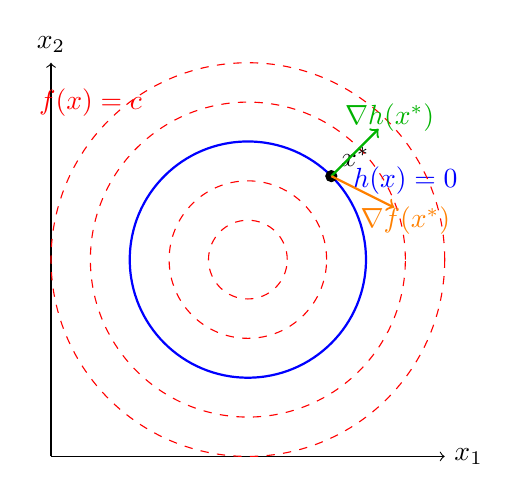
\begin{tikzpicture}
\draw[->] (0,0) -- (5,0) node[right] {$x_1$};
\draw[->] (0,0) -- (0,5) node[above] {$x_2$};

% Kısıt fonksiyonu (bir çember)
\draw[blue,thick] (2.5,2.5) circle (1.5);
\node[blue] at (4.5,3.5) {$h(x) = 0$};

% Amaç fonksiyonunun seviye eğrileri
\draw[red,dashed] (2.5,2.5) circle (0.5);
\draw[red,dashed] (2.5,2.5) circle (1);
\draw[red,dashed] (2.5,2.5) circle (2);
\draw[red,dashed] (2.5,2.5) circle (2.5);
\node[red] at (0.5,4.5) {$f(x) = c$};

% Optimum nokta
\filldraw[black] (3.56,3.56) circle (2pt) node[above right] {$x^*$};

% Gradyanlar
\draw[->,green!70!black,thick] (3.56,3.56) -- (4.16,4.16);
\node[green!70!black] at (4.3,4.3) {$\nabla h(x^*)$};

\draw[->,orange,thick] (3.56,3.56) -- (4.36,3.16);
\node[orange] at (4.5,3) {$\nabla f(x^*)$};

\end{tikzpicture}
\caption{Lagrange çarpanları yönteminin geometrik yorumu: Optimum noktada, amaç fonksiyonunun seviye eğrisi, kısıt fonksiyonunun seviye eğrisine teğettir.}
\label{fig:lagrange_geometry}
\end{figure}

\paragraph{İkinci Dereceden Koşullar}
Bir kritik noktanın gerçekten minimum olup olmadığını belirlemek için, genişletilmiş Hessian matrisinin incelenmesi gerekir. Eğer bu matris, kısıtların teğet uzayında pozitif tanımlı ise, kritik nokta bir yerel minimum olarak kabul edilir.

\begin{tcolorbox}[title=Lagrange Yönteminin Yapısal Optimizasyondaki Uygulamaları]
\begin{itemize}
    \item \textbf{Çelik Çerçeve Yapılar:} Ağırlık minimizasyonu yaparken, düğüm noktalarında kuvvet dengesi ve eleman uygunluğu kısıtlarının sağlanması
    
    \item \textbf{Kompozit Malzeme Tasarımı:} Rijitlik maksimizasyonu yaparken, hacim kısıtı ve malzeme dengesi koşullarının sağlanması
    
    \item \textbf{Kafes Sistemler:} Ağırlık minimizasyonu yaparken, izostatik denge koşullarının sağlanması
    
    \item \textbf{Sonlu Eleman Analizi:} Enerji minimizasyonu prensibine dayalı sonlu eleman formülasyonlarında, kinematik uygunluk ve kuvvet dengesi kısıtlarının sağlanması
\end{itemize}
\end{tcolorbox}

\subsubsection{Karush-Kuhn-Tucker (KKT) Koşulları ve Eşitsizlik Kısıtları}

Karush-Kuhn-Tucker (KKT) koşulları, Lagrange çarpanları yönteminin eşitsizlik kısıtlı problemlere genelleştirilmiş halidir. Bu koşullar, nonlineer programlama alanında optimum çözümlerin karakterizasyonu için temel bir çerçeve sunar.

Eşitsizlik kısıtlı bir optimizasyon problemi şu şekilde ifade edilir:
\begin{equation}
\begin{aligned}
\min & \quad f(x) \\
\text{s.t.} & \quad g_i(x) \leq 0, \quad i = 1, \ldots, m \\
& \quad h_j(x) = 0, \quad j = 1, \ldots, p
\end{aligned}
\end{equation}

Lagrange fonksiyonu bu durumda:
\begin{equation}
\mathcal{L}(x,\lambda,\mu) = f(x) + \sum_{i=1}^m \mu_i g_i(x) + \sum_{j=1}^p \lambda_j h_j(x)
\end{equation}

\paragraph{KKT Koşulları}
Eşitsizlik kısıtlı bir problemin yerel minimumu için gerekli koşullar (KKT koşulları) şunlardır:

\begin{equation}
\begin{aligned}
\nabla f(x^*) + \sum_{i=1}^m \mu_i^* \nabla g_i(x^*) + \sum_{j=1}^p \lambda_j^* \nabla h_j(x^*) &= 0 \\
g_i(x^*) &\leq 0, \quad i = 1, \ldots, m \\
h_j(x^*) &= 0, \quad j = 1, \ldots, p \\
\mu_i^* &\geq 0, \quad i = 1, \ldots, m \\
\mu_i^* g_i(x^*) &= 0, \quad i = 1, \ldots, m
\end{aligned}
\end{equation}

Son koşul "tamamlayıcı gevşeklik" olarak bilinir ve bir kısıtın ya aktif olması (eşitlik olarak sağlanması) ya da ilgili Lagrange çarpanının sıfır olması gerektiğini ifade eder.

\begin{tcolorbox}[title=KKT Koşullarının Yorumlanması]
\begin{itemize}
    \item \textbf{Stasyonerlik:} Amaç fonksiyonunun gradyanının, aktif kısıtların gradyanlarının doğrusal kombinasyonu olarak ifade edilmesi. Bu, optimum noktada ilerlemenin, en az bir aktif kısıtı ihlal etmeden mümkün olmadığını gösterir.
    
    \item \textbf{Uygunluk:} Tüm kısıtların sağlanması.
    
    \item \textbf{Çift Uygunluk:} Eşitsizlik kısıtları için Lagrange çarpanlarının (Kuhn-Tucker çarpanları) negatif olmaması. Bu, kısıtların yönünün önemli olduğunu gösterir.
    
    \item \textbf{Tamamlayıcı Gevşeklik:} Herhangi bir kısıt aktif değilse (eşitsizlik olarak sağlanıyorsa), ilgili Lagrange çarpanı sıfır olmalıdır. Bu, kısıtın "etkisiz" olduğu anlamına gelir.
\end{itemize}
\end{tcolorbox}

\paragraph{KKT Koşullarının Yapısal Optimizasyondaki Önemi}
Yapısal optimizasyon problemleri genellikle çok sayıda eşitsizlik kısıtı içerir. Örneğin:
\begin{itemize}
    \item Gerilme kısıtları: $\sigma_i \leq \sigma_{izin}$
    \item Deplasman kısıtları: $|u_i| \leq u_{izin}$
    \item Burkulma kısıtları: $P_i \leq P_{cr,i}$
    \item Geometrik kısıtlar: minimum kalınlık, genişlik vb.
\end{itemize}

Bu tür problemlerde, KKT koşulları sadece matematiksel bir araç değil, aynı zamanda fiziksel anlamı olan bir çerçeve sunar. Örneğin, gerilme kısıtına ait Lagrange çarpanı, ilgili noktada birim gerilme artışının, optimal tasarımın ağırlığına etkisini gösterir. Bu, "tasarım duyarlılığı analizi" için temel bir kavramdır.

\begin{marginfigure}
\centering
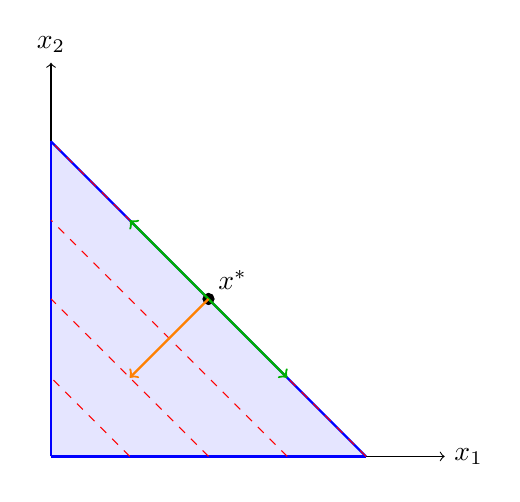
\begin{tikzpicture}
\draw[->] (0,0) -- (5,0) node[right] {$x_1$};
\draw[->] (0,0) -- (0,5) node[above] {$x_2$};

% Uygun bölge
\fill[blue!10] (0,0) -- (0,4) -- (2,2) -- (4,0) -- cycle;
\draw[blue,thick] (0,4) -- (2,2) -- (4,0);
\draw[blue,thick] (0,0) -- (0,4);
\draw[blue,thick] (0,0) -- (4,0);

% Amaç fonksiyonunun seviye çizgileri
\draw[red,dashed] (1,0) -- (0,1);
\draw[red,dashed] (2,0) -- (0,2);
\draw[red,dashed] (3,0) -- (0,3);
\draw[red,dashed] (4,0) -- (0,4);

% Optimum nokta
\filldraw[black] (2,2) circle (2pt) node[above right] {$x^*$};

% Aktif kısıtların gradyanları
\draw[->,green!70!black,thick] (2,2) -- (3,1);
\draw[->,green!70!black,thick] (2,2) -- (1,3);

% Amaç fonksiyonunun gradyanı
\draw[->,orange,thick] (2,2) -- (1,1);

\end{tikzpicture}
\caption{KKT koşullarının geometrik yorumu: Optimum noktada, amaç fonksiyonunun negatif gradyanı, aktif kısıtların gradyanlarının konveks konisinde yer alır.}
\label{fig:kkt_geometry}
\end{marginfigure}

\paragraph{Dualite Teorisi ve Ekonomik Yorum}
Lagrange dualitesi, birincil problem ile onun dual problemi arasındaki ilişkiyi inceler. Dual problem, birincil problemin Lagrange fonksiyonunun minimizasyonu yerine maksimizasyonunu içerir:

\begin{equation}
\begin{aligned}
\max_{\mu \geq 0, \lambda} \min_{x} \mathcal{L}(x,\lambda,\mu)
\end{aligned}
\end{equation}

Dualite teoremi, konveks bir birincil problem için, dual problemin optimal değerinin, birincil problemin optimal değerine eşit olduğunu ifade eder (güçlü dualite). Bu teorem, pek çok optimizasyon algoritmasının temelini oluşturur.

Ekonomik açıdan, dual değişkenler (Lagrange çarpanları) "gölge fiyatları" temsil eder. Yapısal optimizasyonda bu, bir kısıtın marjinal değişiminin, optimal tasarımın değerine etkisini gösterir. Bu yorum, mühendislere hangi kısıtların tasarım üzerinde en büyük etkiye sahip olduğunu anlama imkanı verir.

\begin{tcolorbox}[title=Dualite ve Yapısal Analiz Arasındaki İlişki]
Yapısal mekanikte, potansiyel enerji minimizasyonu (deplasman yöntemi) ve tamamlayıcı enerji minimizasyonu (kuvvet yöntemi) arasındaki ilişki, optimizasyon teorisindeki dualite kavramına mükemmel bir örnektir. 

Bir yapının analizi için:
\begin{itemize}
    \item \textbf{Birincil Problem (Deplasman Yöntemi):} Uyumlu deplasman alanını bulmak için potansiyel enerjiyi minimize etmek
    \item \textbf{Dual Problem (Kuvvet Yöntemi):} Dengedeki kuvvet dağılımını bulmak için tamamlayıcı enerjiyi minimize etmek
\end{itemize}

Bu dualite, yapısal optimizasyon algoritmalarının tasarımında da kullanılır. Özellikle "primal-dual" yöntemler, hem birincil hem de dual problemi eşzamanlı olarak çözerek, daha verimli optimizasyon sağlar.
\end{tcolorbox}

\subsection{Doğrusal ve Kuadratik Programlama}

Klasik optimizasyon yöntemlerinin önemli bir alt kümesi, doğrusal ve kuadratik programlama yöntemleridir. Bu yöntemler, belirli yapıdaki optimizasyon problemleri için özel olarak geliştirilmiş, verimli çözüm algoritmaları sunar.

\subsubsection{Doğrusal Programlama ve Yapısal Uygulamaları}

Doğrusal programlama (DP), hem amaç fonksiyonu hem de kısıtların doğrusal olduğu optimizasyon problemlerini inceler. Standart form:

\begin{equation}
\begin{aligned}
\min & \quad c^T x \\
\text{s.t.} & \quad Ax = b \\
& \quad x \geq 0
\end{aligned}
\end{equation}

Doğrusal programlama, 1940'larda George Dantzig'in Simplex algoritmasını geliştirmesiyle büyük bir ilerleme kaydetmiştir. Günümüzde, büyük ölçekli doğrusal programlama problemleri için İç Nokta Yöntemleri de yaygın olarak kullanılmaktadır.

\paragraph{Simplex Yöntemi ve Geometrik Yorumu}
Simplex yöntemi, uygun bölgenin köşe noktalarını (uç noktaları) sistematik olarak inceleyerek optimum çözümü bulmayı amaçlar. DP'nin temel teoremi, optimal çözümün uygun bölgenin bir köşe noktasında olması gerektiğini ifade eder (eğer çözüm tekil değilse).

Bu yöntemin adımları:
\begin{itemize}
    \item Başlangıç için bir uygun köşe noktası bulunur
    \item Amaç fonksiyonu değerini iyileştirecek komşu köşe noktasına geçilir
    \item Daha iyi bir komşu köşe bulunamayana kadar devam edilir
\end{itemize}



\begin{tcolorbox}[title=Yapısal Mühendislikte DP Uygulamaları]
\begin{itemize}
    \item \textbf{Plastik Limit Analizi:} Yapıların göçme yükünün belirlenmesi, plastik mafsal dağılımının optimizasyonu
    
    \item \textbf{Kafes Sistemlerin Minimum Ağırlık Tasarımı:} Eleman kesitlerinin optimizasyonunda, lineer davranış ve statik yük koşulları altında
    
    \item \textbf{Yapısal Kaynak Dağıtımı:} Sınırlı malzeme veya bütçe koşullarında, yapısal performansı maksimize edecek kaynak dağılımı
    
    \item \textbf{Ulaşım Ağı Optimizasyonu:} Köprü ve yol sistemlerinin yerleşiminin optimizasyonu, trafik akışının modellenmesi
\end{itemize}
\end{tcolorbox}

\paragraph{Plastik Limit Analizi Örneği}
Plastik limit analizi, doğrusal programlamanın yapısal mühendislikteki en önemli uygulamalarından biridir. Statik teorem (alt sınır) formülasyonu:
\begin{equation}
\begin{aligned}
\max & \quad \lambda \\
\text{s.t.} & \quad B^T q = \lambda F + F_0 \\
& \quad |q_i| \leq q_i^p, \quad i = 1, \ldots, n
\end{aligned}
\end{equation}

Burada:
\begin{itemize}
    \item $\lambda$: yük çarpanı
    \item $q$: iç kuvvetler vektörü
    \item $B$: denge matrisi
    \item $F$: değişken dış yük vektörü
    \item $F_0$: sabit dış yük vektörü
    \item $q_i^p$: eleman $i$ için plastik limit kapasitesi
\end{itemize}

Bu formülasyon, yapının göçmeden dayanabileceği maksimum yük çarpanını belirler.

\sidenote{Plastik limit analizi, özellikle çelik yapıların tasarımında önemlidir. Yapının elastik sınırın ötesinde, plastik deformasyon kapasitesini kullanarak dayanabildiği maksimum yükü belirleyerek, daha ekonomik tasarımlar elde edilmesini sağlar.}

\begin{marginfigure}
\centering
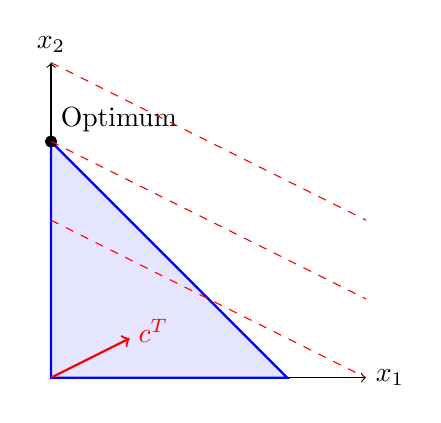
\begin{tikzpicture}
\draw[->] (0,0) -- (4,0) node[right] {$x_1$};
\draw[->] (0,0) -- (0,4) node[above] {$x_2$};

% Kısıtlar ve uygun bölge
\fill[blue!10] (0,0) -- (0,3) -- (1,2) -- (3,0) -- cycle;
\draw[blue,thick] (0,0) -- (0,3) -- (1,2) -- (3,0) -- cycle;

% Amaç fonksiyonu vektörü
\draw[->,red,thick] (0,0) -- (1,0.5);
\node[red] at (1.3,0.6) {$c^T$};

% Optimum nokta
\filldraw[black] (0,3) circle (2pt) node[above right] {Optimum};

% Amaç fonksiyonunun seviye çizgileri
\draw[red,dashed] (0,4) -- (4,2);
\draw[red,dashed] (0,3) -- (4,1);
\draw[red,dashed] (0,2) -- (4,0);

\end{tikzpicture}
\caption{Doğrusal programlamada uygun bölge ve optimum nokta}
\label{fig:linear_programming}
\end{marginfigure}

\subsubsection{Kuadratik Programlama}

Kuadratik programlama (KP), amaç fonksiyonunun ikinci dereceden, kısıtların ise doğrusal olduğu optimizasyon problemlerini ele alır:

\begin{equation}
\begin{aligned}
\min & \quad \frac{1}{2}x^TQx + c^Tx \\
\text{s.t.} & \quad Ax = b \\
& \quad x \geq 0
\end{aligned}
\end{equation}

Burada $Q$, simetrik bir matristir. Eğer $Q$ pozitif (yarı) tanımlı ise, problem konvekstir ve global optimumu bulmak göreceli olarak kolaydır.

\paragraph{Çözüm Yöntemleri}
Kuadratik programlama problemleri için çeşitli çözüm yöntemleri geliştirilmiştir:
\begin{itemize}
    \item \textbf{Aktif Set Yöntemleri:} Hangi kısıtların aktif olduğuna dair tahminler yaparak, kısıtsız optimizasyon alt problemlerini çözer
    
    \item \textbf{İç Nokta Yöntemleri:} Uygun bölgenin içinden geçerek, optimum noktaya yaklaşır
    
    \item \textbf{Sıralı Kuadratik Programlama (SQP):} Nonlineer optimizasyon problemlerini, kuadratik alt problemlere bölerek çözer
\end{itemize}



\begin{tcolorbox}[title=Yapısal Mühendislikte KP Uygulamaları]
\begin{itemize}
    \item \textbf{Elastik Deformasyon Minimizasyonu:} Yapının rijitlik matrisini kullanarak, belirli yükler altında deformasyonu minimize etmek
    
    \item \textbf{Dinamik Davranış Optimizasyonu:} Yapının kütle ve rijitlik matrislerini kullanarak, dinamik tepkiyi optimize etmek
    
    \item \textbf{Sonlu Eleman Modeli Kalibrasyonu:} Deneysel ve sayısal veriler arasındaki farkın karelerini minimize etmek
    
    \item \textbf{Ağırlık ve Deplasman Optimizasyonu:} Hem ağırlığı hem de deplasman enerjisini içeren çok amaçlı optimizasyon
\end{itemize}
\end{tcolorbox}

\paragraph{Yapısal Esneklik (Compliance) Minimizasyonu Örneği}
Yapısal tasarımda sıkça karşılaşılan bir kuadratik programlama problemi, belirli bir hacim kısıtı altında esnekliğin (veya deformasyon enerjisinin) minimizasyonudur:

\begin{equation}
\begin{aligned}
\min & \quad \frac{1}{2}F^Tu \\
\text{s.t.} & \quad Ku = F \\
& \quad \sum_{e=1}^{n_e} v_e\rho_e \leq V \\
& \quad 0 \leq \rho_e \leq 1, \quad e = 1, \ldots, n_e
\end{aligned}
\end{equation}

Burada:
\begin{itemize}
    \item $u$: deplasman vektörü
    \item $F$: kuvvet vektörü
    \item $K$: global rijitlik matrisi
    \item $\rho_e$: eleman $e$ için malzeme yoğunluğu (tasarım değişkeni)
    \item $v_e$: eleman $e$'nin hacmi
    \item $V$: izin verilen toplam hacim
\end{itemize}

Bu formülasyon, topoloji optimizasyonunun temelini oluşturur ve SIMP (Solid Isotropic Material with Penalization) metodunun başlangıç noktasıdır.

\subsection{Modern Klasik Optimizasyon Algoritmaları}

Klasik optimizasyon yöntemlerinin modern uzantıları, çeşitli yaklaşımlar kullanarak büyük ve karmaşık yapısal optimizasyon problemlerini çözmeyi amaçlar. Bu bölümde, klasik yöntemlerin daha gelişmiş versiyonlarını ele alacağız.

\subsubsection{Sekant Yöntemleri ve Yapısal Uygulamaları}

Sekant yöntemleri, Newton yönteminin Hessian matrisini hesaplama gereksinimini ortadan kaldırmak için geliştirilen yaklaşımlardır. Bu yöntemler, gradyan bilgisini kullanarak Hessian matrisinin yaklaşık bir tahminini oluşturur.

En yaygın sekant yöntemleri şunlardır:
\begin{itemize}
    \item \textbf{Broyden Yöntemi:} Genel nonlineer denklem sistemlerinin çözümünde kullanılır
    \item \textbf{DFP (Davidon-Fletcher-Powell) Yöntemi:} Quasi-Newton yöntemlerinin ilk örneklerindendir
    \item \textbf{BFGS (Broyden-Fletcher-Goldfarb-Shanno) Yöntemi:} Yapısal optimizasyon dahil birçok alanda standart haline gelmiştir
\end{itemize}

BFGS yönteminde, Hessian matrisinin yaklaşık değeri şu şekilde güncellenir:
\begin{equation}
B_{k+1} = B_k - \frac{B_k s_k s_k^T B_k}{s_k^T B_k s_k} + \frac{y_k y_k^T}{y_k^T s_k}
\end{equation}

Burada:
\begin{itemize}
    \item $s_k = x_{k+1} - x_k$
    \item $y_k = \nabla f(x_{k+1}) - \nabla f(x_k)$
\end{itemize}

BFGS yöntemi, yapısal optimizasyon problemlerinde, özellikle çok sayıda tasarım değişkeni söz konusu olduğunda yaygın kullanılır.

\paragraph{BFGS'in Yapısal Optimizasyondaki Avantajları}
\begin{itemize}
    \item \textbf{Bellek Verimliliği:} L-BFGS varyantı ile büyük ölçekli problemlerde bile uygulanabilir
    \item \textbf{Süper Lineer Yakınsama:} Optimum noktaya yaklaştıkça, yakınsama hızı artar
    \item \textbf{Sayısal Stabilite:} Newton yöntemine göre daha kararlıdır
    \item \textbf{Line Search ile Entegrasyon:} Güçlü line search stratejileriyle birleştirilebilir
\end{itemize}

\subsubsection{Trust Region ve Line Search Stratejileri}

Gradyan tabanlı optimizasyon yöntemlerinin performansı, adım boyutu seçimine büyük ölçüde bağlıdır. Line search ve trust region, adım boyutunu belirlemek için geliştirilen iki temel stratejidir.

\paragraph{Line Search Stratejileri}
Line search yöntemlerinde, arama yönü $d_k$ belirlendikten sonra, uygun adım boyutu $\alpha_k$ bulunur:
\begin{equation}
x_{k+1} = x_k + \alpha_k d_k
\end{equation}

Optimal adım boyutunu belirlemek için çeşitli kriterler kullanılır:
\begin{itemize}
    \item \textbf{Armijo Koşulu:} Adım boyutunun, fonksiyon değerinde yeterli azalma sağlamasını garantiler
    \item \textbf{Wolfe Koşulları:} Armijo koşuluna ek olarak, gradyan değişiminin belirli bir oranı sağlamasını gerektirir
    \item \textbf{Goldstein Koşulları:} Hem fonksiyon değerinde azalma hem de adım boyutunun çok küçük olmamasını sağlar
\end{itemize}

\paragraph{Trust Region Yaklaşımı}
Trust region yöntemlerinde, modelin güvenilir olduğu bir bölge tanımlanır ve bu bölge içinde model minimize edilir:
\begin{equation}
\begin{aligned}
\min & \quad m_k(p) = f_k + g_k^Tp + \frac{1}{2}p^TB_kp \\
\text{s.t.} & \quad \|p\| \leq \Delta_k
\end{aligned}
\end{equation}

Burada:
\begin{itemize}
    \item $m_k(p)$: $k$. iterasyonda fonksiyonun kuadratik modeli
    \item $f_k = f(x_k)$, $g_k = \nabla f(x_k)$
    \item $B_k$: Hessian matrisi veya yaklaşımı
    \item $\Delta_k$: trust region yarıçapı
\end{itemize}

Her iterasyonda, model tahmini ile gerçek fonksiyon değişimi karşılaştırılarak, trust region yarıçapı güncellenir.

\begin{tcolorbox}[title=Yapısal Mühendislikte Trust Region Uygulamaları]
Trust region yaklaşımı, yapısal mühendislikte özellikle şu durumlarda tercih edilir:
\begin{itemize}
    \item \textbf{Kötü Koşullu Problemler:} Rijitlik matrisinin koşul sayısının yüksek olduğu durumlarda
    \item \textbf{Doğrusal Olmayan Davranış:} Malzeme veya geometrik nonlineerite içeren yapısal analizlerde
    \item \textbf{Kararsız Sistemler:} Burkulma analizi gibi kararsızlık noktalarına yakın problemlerde
    \item \textbf{Çoklu Fizik Analizleri:} Termal-yapısal, akışkan-yapı etkileşimi gibi karmaşık multifizik problemlerde
\end{itemize}
\end{tcolorbox}

\subsubsection{Sıralı Kısıt Programlama}

Sıralı Kısıt Programlama (Sequential Constraint Programming - SCP), yapısal optimizasyon problemlerinin çözümü için geliştirilen etkili bir yaklaşımdır. Bu yöntem, nonlineer problemi, bir dizi doğrusal alt probleme dönüştürerek çözer.

SCP'nin temel yaklaşımı:
\begin{itemize}
    \item Nonlineer kısıtları, mevcut iterasyon noktası etrafında doğrusallaştırır
    \item Doğrusallaştırılmış problemi çözer
    \item Çözümü yeni bir iterasyon noktası olarak kullanır
    \item Yakınsama sağlanana kadar tekrarlar
\end{itemize}

Bu yöntem, MMA (Method of Moving Asymptotes) gibi daha gelişmiş varyantlarıyla, yapısal topoloji optimizasyonunda yaygın olarak kullanılmaktadır.


MMA'nın yapısal optimizasyondaki başlıca avantajları:
\begin{itemize}
    \item Büyük ölçekli topoloji optimizasyonu problemlerinde verimlilik
    \item Doğrusal olmayan kısıtları etkin bir şekilde ele alabilme
    \item Salınımları azaltarak kararlı yakınsama sağlama
    \item Paralel hesaplamaya uygunluk
\end{itemize}

\begin{figure}
\centering
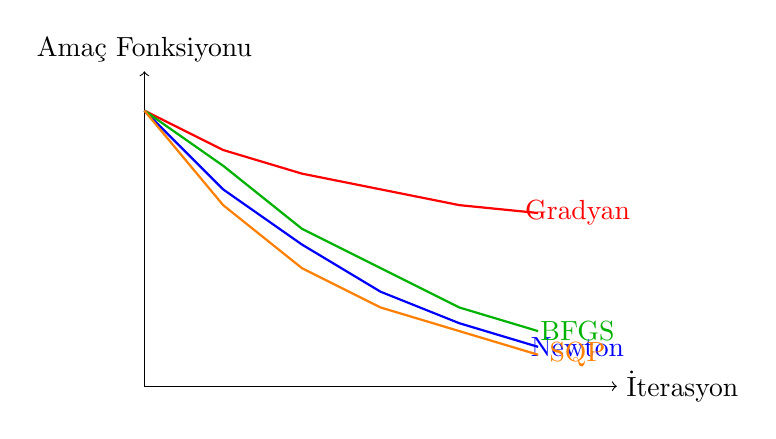
\begin{tikzpicture}
\draw[->] (0,0) -- (6,0) node[right] {İterasyon};
\draw[->] (0,0) -- (0,4) node[above] {Amaç Fonksiyonu};

% Gradyan iniş
\draw[red,thick] plot coordinates {(0,3.5) (1,3.0) (2,2.7) (3,2.5) (4,2.3) (5,2.2)};
\node[red] at (5.5,2.2) {Gradyan};

% Newton
\draw[blue,thick] plot coordinates {(0,3.5) (1,2.5) (2,1.8) (3,1.2) (4,0.8) (5,0.5)};
\node[blue] at (5.5,0.5) {Newton};

% BFGS
\draw[green!70!black,thick] plot coordinates {(0,3.5) (1,2.8) (2,2.0) (3,1.5) (4,1.0) (5,0.7)};
\node[green!70!black] at (5.5,0.7) {BFGS};

% SQP
\draw[orange,thick] plot coordinates {(0,3.5) (1,2.3) (2,1.5) (3,1.0) (4,0.7) (5,0.4)};
\node[orange] at (5.5,0.4) {SQP};

\end{tikzpicture}
\caption{Farklı optimizasyon algoritmalarının yakınsama davranışlarının karşılaştırması}
\label{fig:convergence_comparison}
\end{figure}

\subsection{Sonuç ve Modern Yöntemlere Geçiş}

Klasik optimizasyon yöntemleri, yapısal mühendislikte karşılaşılan çeşitli problemlerin çözümünde hala büyük önem taşımaktadır. Bu yöntemler, modern meta-sezgisel algoritmaların ve yapay zeka tabanlı yaklaşımların temelini oluşturur.

\begin{tcolorbox}[title=Klasik ve Modern Yöntemlerin Karşılaştırması]
\begin{itemize}
    \item \textbf{Klasik Yöntemler:} Matematiksel sağlamlık, kesin yakınsama garantileri, verimlilik
    \item \textbf{Modern Yöntemler:} Çok modlu fonksiyonlar için global arama, paralel hesaplama, karmaşık kısıtların ele alınmasında esneklik
\end{itemize}
\end{tcolorbox}

Günümüzde, klasik algoritmaların güçlü yönleri ile modern yaklaşımların esnekliğini birleştiren hibrit yöntemler büyük ilgi görmektedir. Bu hibrit yaklaşımlar, özellikle büyük ölçekli ve çok amaçlı yapısal optimizasyon problemlerinde etkili çözümler sunmaktadır.
  
\section{Benchmark Test Fonksiyonları}
Bu başlık altında incelenen test fonksiyonlarına ait python kodlarına \href{https://github.com/btayfur/structural-optimization/blob/main/Code/Sources/OptimizationBenchmarks}{bağlantıdan} ulaşılabilir. \sidenote{
    
\qrcode[height=1in]{https://github.com/btayfur/structural-optimization/blob/main/Code/Sources/OptimizationBenchmarks}}

Optimizasyon algoritmalarının performansını değerlendirmek ve karşılaştırmak için kullanılan standart test fonksiyonları\sidenote{Test fonksiyonları, algoritmaların güçlü ve zayıf yönlerini ortaya çıkarmada önemli rol oynar. Bir algoritmanın gerçek dünya problemlerindeki başarısı, önce bu test fonksiyonları üzerinde değerlendirilir.}, farklı zorluk derecelerine sahip matematiksel yapılar olarak karşımıza çıkar. Bu test fonksiyonları, bilinen global minimum noktaları, karmaşık yerel minimum yapıları ve çeşitli topolojik özellikleri ile algoritmaları sınamak için tasarlanmıştır.

\subsection{Benchmark Fonksiyonlarının Optimizasyondaki Rolü}

Optimizasyon algoritmalarının performansını değerlendirmek için standart test fonksiyonları kullanılır. Bu fonksiyonlar şu açılardan önem taşır:

\begin{itemize}
    \item \textbf{Karşılaştırılabilirlik:} Farklı algoritmaların aynı problem üzerindeki başarısını objektif olarak değerlendirmeyi sağlar.
    \item \textbf{Güçlü ve Zayıf Yönleri Belirleme:} Algoritmaların hangi tür problemlerde iyi performans gösterdiğini, hangi tür problemlerde zorlandığını gösterir.
    \item \textbf{Algoritma Geliştirme:} Yeni optimizasyon algoritmalarının geliştirilmesi ve iyileştirilmesi sürecinde rehberlik eder.
    \item \textbf{Gerçek Dünya Uygulamalarına Hazırlık:} Algoritmaların daha karmaşık gerçek dünya problemlerine uygulanmadan önce test edilmesini sağlar.
\end{itemize}

İdeal bir benchmark fonksiyonu, gerçek dünyadaki optimizasyon problemlerinin karmaşıklığını yansıtırken, matematiksel olarak anlaşılabilir ve analiz edilebilir olmalıdır. Benchmark fonksiyonları genellikle şu özelliklere göre sınıflandırılır: doğrusallık, modalite (tepe nokta sayısı), süreklilik, türevlenebilirlik, sınırlılık ve boyutsallık.

\subsubsection{Benchmark Fonksiyonlarının Ortak Özellikleri}

Çoğu benchmark fonksiyonu aşağıdaki özelliklere sahiptir:

\begin{itemize}
    \item Bilinen global minimum değeri ve konumu
    \item Matematiksel olarak tanımlanmış yapı
    \item Ayarlanabilir boyut (genellikle çok boyutlu uzaylara genişletilebilir)
    \item Çeşitli zorluklar (örn. yerel minimumlar, düz bölgeler, dik vadiler)
    \item Önerilen arama aralıkları
\end{itemize}

\subsection{Çok Modlu ve Tek Modlu Test Fonksiyonları}

Test fonksiyonları, içerdikleri tepe noktası (mod) sayısına göre tek modlu (unimodal) ve çok modlu (multimodal) olarak ikiye ayrılır.

\subsubsection{Tek Modlu Fonksiyonlar}

Tek modlu fonksiyonlar, yalnızca bir tane global minimuma sahiptir ve genellikle daha basit yapıdadır. Bu fonksiyonlar, algoritmanın yakınsama hızını ve hassasiyetini test etmek için kullanılır. Örnek olarak:

\begin{itemize}
    \item \textbf{Sphere Fonksiyonu:} Matematiksel olarak en basit optimizasyon test fonksiyonudur ve şu şekilde tanımlanır:
    \begin{equation}
        f(\mathbf{x}) = \sum_{i=1}^{n} x_i^2
    \end{equation}
    Global minimum $f(\mathbf{x}^*) = 0$, $\mathbf{x}^* = (0, 0, \ldots, 0)$ noktasında yer alır.
    
    \item \textbf{Booth Fonksiyonu:} İki boyutlu, çanak şeklinde bir fonksiyondur:
    \begin{equation}
        f(x, y) = (x + 2y - 7)^2 + (2x + y - 5)^2
    \end{equation}
    Global minimum $f(1, 3) = 0$ noktasındadır.
\end{itemize}

\subsubsection{Çok Modlu Fonksiyonlar}

Çok modlu fonksiyonlar, birden fazla yerel minimuma sahiptir ve bu nedenle algoritmaların yerel minimumlara takılmadan global minimumu bulabilme yeteneğini test eder. Bu fonksiyonlar, özellikle metasezgisel ve evrimsel algoritmaların performansını değerlendirmek için önemlidir. Önemli örnekler arasında:

\begin{itemize}
    \item \textbf{Ackley Fonksiyonu:} Çok sayıda yerel minimumu olan karmaşık bir test fonksiyonudur. Matematiksel olarak şöyle tanımlanır:
    \begin{equation}
        f(\mathbf{x}) = -20\exp\left(-0.2\sqrt{\frac{1}{n}\sum_{i=1}^{n}x_i^2}\right) - \exp\left(\frac{1}{n}\sum_{i=1}^{n}\cos(2\pi x_i)\right) + 20 + e
    \end{equation}
    
    Bu fonksiyonun global minimumu $f(\mathbf{x}^*) = 0$, $\mathbf{x}^* = (0, 0, \ldots, 0)$ noktasında bulunur. Genellikle $[-32.768, 32.768]$ aralığında tanımlanır.
    
    \item \textbf{Rastrigin Fonksiyonu:} Sinüzoidal modülasyonu ile çok sayıda yerel minimuma sahip zorlayıcı bir fonksiyondur:
    \begin{equation}
        f(\mathbf{x}) = 10n + \sum_{i=1}^{n} \left[ x_i^2 - 10\cos(2\pi x_i) \right]
    \end{equation}
    Global minimum $f(\mathbf{x}^*) = 0$, $\mathbf{x}^* = (0, 0, \ldots, 0)$ noktasındadır.
\end{itemize}

\begin{figure}[h]
    \centering
    \includegraphics[width=0.8\textwidth]{weeks_new/imgs/ackley_function.png}
    \caption{Ackley fonksiyonunun 3B gösterimi (soldaki) ve kontur grafiği (sağdaki). Fonksiyonun merkezde bir global minimum ve etrafında çok sayıda yerel minimum içeren yapısı dikkat çekicidir.}
    \label{fig:ackley}
\end{figure}

\subsubsection{Ackley Fonksiyonu: Derinlemesine İnceleme}

Ackley fonksiyonu, David Ackley tarafından 1987 yılında önerilmiş ve optimizasyon algoritmaları için standart bir test fonksiyonu haline gelmiştir. Fonksiyonun matematiksel yapısı şu özellikleri ortaya çıkarır:

\begin{itemize}
    \item \textbf{Neredeyse düz bölgeler:} Merkezden uzaklaştıkça fonksiyon neredeyse düz bir yapıya sahiptir, bu da gradyan tabanlı yöntemlerin doğru yönü belirlemesini zorlaştırır.
    
    \item \textbf{Periyodik dalgalanmalar:} Kosinüs terimi nedeniyle, fonksiyon yüzeyi düzenli aralıklarla iniş ve çıkışlar gösterir, çok sayıda yerel minimum oluşturur.
    
    \item \textbf{Merkezdeki derin çukur:} Global minimum etrafında dik bir çukur bulunur, bu da algoritmanın optimuma yakın olduğunda hassas adımlar atmasını gerektirir.
\end{itemize}

Ackley fonksiyonu, özellikle şu tür algoritmaların test edilmesinde etkilidir:

\begin{itemize}
    \item Yerel aramayla global arama stratejilerini dengeleyen metasezgisel algoritmalar
    \item Çok sayıda yerel minimumdan kaçabilme yeteneğine sahip algoritmalar
    \item Farklı çözüm bölgelerini aynı anda keşfedebilen popülasyon tabanlı algoritmalar
\end{itemize}

$n$-boyutlu Ackley fonksiyonunun optimizasyonu şu zorlukları içerir:
\begin{itemize}
    \item Boyut arttıkça yerel minimum sayısı üstel olarak artar
    \item Merkeze yakın bölgelerde yüksek hassasiyet gerektirir
    \item Düz bölgelerde gradyan bilgisi yetersiz kalır
\end{itemize}

\begin{tcolorbox}[title=Ackley Fonksiyonu Optimizasyon Zorluğu]
Ackley fonksiyonu, hem keşif (exploration) hem de yararlanma (exploitation) özelliklerini aynı anda test eder:
\begin{itemize}
    \item Keşif: Geniş, neredeyse düz bölgelerde doğru yönü bulabilme
    \item Yararlanma: Merkezdeki dik çukurda hassas ayarlamaları yapabilme
    \item Denge: Yerel minimumlardan kaçarken global minimuma yakınsayabilme
\end{itemize}
\end{tcolorbox}

\subsection{Yüksek Boyutlu Optimizasyon Problemleri}

\subsubsection{Boyut Artışının Etkileri}
\begin{itemize}
    \item Arama uzayı üstel olarak büyür
    \item Hesaplama maliyeti artar
    \item Lokal minimum sayısı artar
    \item Yakınsama zorlaşır
\end{itemize}

Yüksek boyutlu optimizasyon problemleri, gerçek dünyadaki birçok mühendislik uygulamasında karşımıza çıkar. Boyut artışı, "boyutun laneti" (curse of dimensionality) olarak bilinen fenomene yol açar. Bu fenomen, boyut arttıkça arama uzayının üstel olarak büyümesi ve algoritmaların etkinliğinin dramatik biçimde azalması ile karakterize edilir.

\subsubsection{Boyutun Lanetinin Etkileri}

Boyut artışının optimizasyon süreci üzerindeki etkileri:

\begin{itemize}
    \item \textbf{Arama uzayı genişliği:} $n$ boyutlu ve her boyutta $m$ ayrık nokta içeren bir problemde, toplam arama uzayı $m^n$ büyüklüğündedir. Örneğin, her boyutta 10 nokta için, 2 boyutlu problemde 100 nokta, 10 boyutlu problemde $10^{10}$ nokta, 100 boyutlu problemde $10^{100}$ nokta vardır.
    
    \item \textbf{Veri seyrekliği:} Yüksek boyutlarda, veri noktaları arasındaki mesafeler artar ve veri seyrekleşir. Bu, algoritmaların doğru yönü belirlemesini zorlaştırır.
    
    \item \textbf{Örnekleme zorluğu:} Yüksek boyutlu uzayı yeterince örneklemek için gereken nokta sayısı, pratikte ulaşılamayacak kadar büyüktür.
\end{itemize}

\subsubsection{Yüksek Boyutlu Test Fonksiyonları}

Bazı test fonksiyonları özellikle yüksek boyutlu problemlerde algoritmaların performansını değerlendirmek için tasarlanmıştır:

\begin{itemize}
    \item \textbf{Rosenbrock Fonksiyonu:} Dar bir vadi boyunca ilerleyen ve boyut arttıkça zorlaşan bir fonksiyondur:
    \begin{equation}
        f(\mathbf{x}) = \sum_{i=1}^{n-1} \left[ 100(x_{i+1} - x_i^2)^2 + (x_i - 1)^2 \right]
    \end{equation}
    
    \item \textbf{Schwefel Fonksiyonu:} Yüksek boyutlarda çok sayıda geniş bölgeli yerel minimuma sahiptir:
    \begin{equation}
        f(\mathbf{x}) = 418.9829n - \sum_{i=1}^{n} x_i\sin(\sqrt{|x_i|})
    \end{equation}
\end{itemize}

\subsection{Stokastik Algoritmaların Test Edilmesi}

Stokastik algoritmalar, deterministik olmayan, rastgele elemanlara sahip algoritmalardır. Bu algoritmalar her çalıştırıldıklarında farklı sonuçlar üretebilirler. Metasezgisel algoritmalar, evrimsel algoritmalar ve yapay sinir ağları gibi modern optimizasyon yöntemleri genellikle stokastik karaktere sahiptir.

\subsubsection{Stokastik Algoritmaların Test Prensipleri}

\begin{itemize}
    \item \textbf{Çoklu çalıştırma:} Her test fonksiyonu için algoritma birden çok kez (genellikle 30-50 bağımsız çalıştırma) çalıştırılmalıdır.
    
    \item \textbf{İstatistiksel analiz:} Sonuçların ortalaması, standart sapması, medyanı, en iyi ve en kötü değerleri raporlanmalıdır.
    
    \item \textbf{Yakınsama analizi:} Algoritmanın zaman içindeki davranışı, iterasyon/değerlendirme sayısına karşı en iyi değer grafiği ile gösterilmelidir.
    
    \item \textbf{Parametre duyarlılığı:} Algoritmanın parametre değişimlerine olan duyarlılığı test edilmelidir.
\end{itemize}

\subsection{Test Prensipleri}

Optimizasyon algoritmalarının adil ve kapsamlı bir şekilde değerlendirilmesi için bazı temel prensiplere uyulmalıdır:

\begin{itemize}
    \item \textbf{Çeşitlilik:} Farklı özelliklere sahip test fonksiyonları kullanılmalıdır.
    
    \item \textbf{Adil karşılaştırma:} Karşılaştırılan tüm algoritmalar için aynı koşullar (başlangıç noktaları, fonksiyon değerlendirme sayısı, sonlandırma kriterleri) sağlanmalıdır.
    
    \item \textbf{Yeterli tekrar:} Stokastik algoritmalar için yeterli sayıda bağımsız çalıştırma yapılmalıdır.
    
    \item \textbf{Boyut değişimi:} Algoritmaların farklı problem boyutlarındaki performansı test edilmelidir.
    
    \item \textbf{Kapsamlı raporlama:} Sadece ortalama veya en iyi değerler değil, tam istatistiksel sonuçlar raporlanmalıdır.
\end{itemize}

\subsection{Performans Ölçütleri}

Optimizasyon algoritmalarının performansı çeşitli ölçütlerle değerlendirilebilir. Bu ölçütler, sayısal ve kalite olmak üzere iki ana kategoriye ayrılabilir.

\subsubsection{Sayısal Ölçütler}

\begin{itemize}
    \item \textbf{Yakınsama hızı:} Algoritmanın istenen çözüme ne kadar hızlı ulaştığını gösterir. Genellikle fonksiyon değerlendirme sayısı veya iterasyon sayısı olarak ölçülür.
    
    \item \textbf{Hassasiyet:} Bulunan çözümün bilinen global optimuma ne kadar yakın olduğunu gösterir. Genellikle mutlak veya göreceli hata olarak ölçülür.
    
    \item \textbf{Başarı oranı:} Algoritmanın kabul edilebilir bir çözüme ulaşma yüzdesidir. Özellikle stokastik algoritmalar için önemlidir.
    
    \item \textbf{Hesaplama karmaşıklığı:} Algoritmanın çalışma süresi veya bellek kullanımı olarak ölçülebilir.
\end{itemize}

\subsubsection{Kalite Ölçütleri}

\begin{itemize}
    \item \textbf{Sağlamlık (robustness):} Algoritmanın farklı problem tiplerine, başlangıç koşullarına ve parametre değişimlerine karşı duyarlılığı.
    
    \item \textbf{Genellenebilirlik:} Algoritmanın farklı problem sınıflarında gösterdiği performans.
    
    \item \textbf{Ölçeklenebilirlik:} Problem boyutu arttıkça algoritmanın performansındaki değişim.
    
    \item \textbf{Keşif-yararlanma dengesi:} Algoritmanın global arama (keşif) ve yerel iyileştirme (yararlanma) arasındaki dengeyi sağlama yeteneği.
\end{itemize}

\sidenote{Performans ölçütleri, farklı algoritmaların objektif olarak karşılaştırılmasını sağlar. Ancak, tek bir ölçüt yerine birden fazla ölçütün birlikte değerlendirilmesi daha sağlıklıdır.}

\begin{tcolorbox}[title=No Free Lunch Teoremi]
Hiçbir optimizasyon algoritması tüm problemlerde en iyi performansı gösteremez:
\begin{itemize}
    \item Her algoritmanın güçlü ve zayıf yönleri vardır
    \item Problem yapısına uygun algoritma seçimi önemlidir
    \item Hibrit yaklaşımlar avantajlı olabilir
\end{itemize}
\end{tcolorbox}

\subsubsection{Benchmark Sonuçlarının Sunumu}

Benchmark test sonuçlarının etkili sunumu için şu yöntemler kullanılabilir:

\begin{itemize}
    \item \textbf{Tablo formatı:} Algoritmaların her test fonksiyonu için ortalama, standart sapma, en iyi ve en kötü değerlerini gösteren tablolar.
    
    \item \textbf{Yakınsama grafikleri:} İterasyon/değerlendirme sayısına karşı en iyi değerin değişimini gösteren grafikler.
    
    \item \textbf{Kutu grafikleri (Box plots):} Sonuçların dağılımını ve medyan, çeyrekler gibi istatistiksel özetleri görsel olarak sunan grafikler.
    
    \item \textbf{Sıralama tabloları:} Algoritmaların her bir test fonksiyonu için performans sıralamasını gösteren tablolar.
    
    \item \textbf{İstatistiksel anlamlılık testleri:} Algoritmaların performans farklarının istatistiksel olarak anlamlı olup olmadığını gösteren testler (t-testi, Wilcoxon işaretli sıra testi, Friedman testi vb.).
\end{itemize}

\subsection{Benchmark Fonksiyonlarının Kategorileri}

Farklı özelliklere sahip benchmark fonksiyonları, algoritmaların çeşitli zorluklarla başa çıkma yeteneğini test eder. Burada, temel fonksiyon kategorileri ve örnekleri verilmiştir:

\subsubsection{Çok Sayıda Yerel Minimuma Sahip Fonksiyonlar}

Bu fonksiyonlar, algoritmalar için bir zorluk oluşturan birçok yerel minimuma sahiptir ve global optimizasyon yeteneğini test eder:

\begin{itemize}
    \item Ackley
    \item Rastrigin
    \item Griewank
    \item Schwefel
    \item Levy
    \item Shubert
\end{itemize}

\subsubsection{Çanak Şeklindeki Fonksiyonlar}

Bu fonksiyonlar, dairesel veya eliptik konturlarla çevrili tek bir minimuma sahiptir ve yerel optimizasyon yeteneğini test eder:

\begin{itemize}
    \item Sphere
    \item Bohachevsky
    \item Sum Squares
    \item Rotated Hyper-Ellipsoid
\end{itemize}

\subsubsection{Tabak Şeklindeki Fonksiyonlar}

Bu fonksiyonlar, algoritmaların doğru yönü belirleme yeteneğini zorlayabilen düz bölgelere sahiptir:

\begin{itemize}
    \item Booth
    \item Matyas
    \item Zakharov
    \item McCormick
\end{itemize}

\subsubsection{Vadi Şeklindeki Fonksiyonlar}

Bu fonksiyonlar, birçok algoritmanın yakınsamasını yavaşlatabilen uzun, dar vadilere sahiptir:

\begin{itemize}
    \item Rosenbrock (Muz Fonksiyonu)
    \item Six-Hump Camel
    \item Three-Hump Camel
    \item Dixon-Price
\end{itemize}

\subsubsection{Dik Sırtlar/Düşüşler İçeren Fonksiyonlar}

Bu fonksiyonlar, gradyan tabanlı yöntemleri zorlayabilecek dik sırtlara veya düşüşlere sahiptir:

\begin{itemize}
    \item Easom
    \item Michalewicz
    \item De Jong N.5
\end{itemize}

\subsection{Sonuç ve Uygulamalar}

Benchmark test fonksiyonları, optimizasyon algoritmalarının geliştirilmesi, test edilmesi ve karşılaştırılması için vazgeçilmez araçlardır. Bu fonksiyonlar, algoritmaların farklı problem tiplerindeki performansını değerlendirmeye ve zayıf yönlerini belirlemeye yardımcı olur.

\begin{itemize}
    \item \textbf{Algoritma geliştirmede:} Yeni algoritmaların güçlü ve zayıf yönlerinin belirlenmesi
    \item \textbf{Parametre ayarlamada:} Algoritma parametrelerinin optimizasyonu
    \item \textbf{Hibrit yaklaşımlarda:} Farklı algoritmaların güçlü yönlerini birleştiren hibrit yöntemlerin geliştirilmesi
    \item \textbf{Eğitimde:} Optimizasyon algoritmalarının davranışlarının anlaşılması
    \item \textbf{Gerçek dünya problemlerine hazırlıkta:} Daha karmaşık problemlere geçmeden önce algoritmaların temel yeteneklerinin değerlendirilmesi
\end{itemize}

  
\section{Metaheuristic Optimization Algorithms I}
Nature-inspired modern algorithms used in solving complex optimization problems will be discussed in this section. These algorithms provide effective solutions when classical methods prove insufficient.

\subsection{Basic Characteristics of Metaheuristic Algorithms}

Metaheuristic algorithms are nature-inspired methods used in solving complex optimization problems:

\begin{itemize}
    \item Have stochastic characteristics
    \item Problem-independent structure
    \item Do not require gradient information
    \item Potential to reach global optimum
\end{itemize}

\sidenote{The most important characteristic of metaheuristic algorithms is their potential to reach the global optimum without getting stuck in local optima in complex and multimodal problems.}

\subsection{Differences Between Deterministic and Stochastic Algorithms}

\begin{tcolorbox}[title=Deterministic vs Stochastic]
\begin{itemize}
    \item \textbf{Deterministic:}
        \begin{itemize}
            \item Same starting point → Same result
            \item Gradient-based
            \item Fast convergence to local optimum
        \end{itemize}
    \item \textbf{Stochastic:}
        \begin{itemize}
            \item Random search
            \item Different result in each run
            \item Global optimum potential
        \end{itemize}
\end{itemize}
\end{tcolorbox}

\subsection{Classification of Metaheuristic Algorithms Based on Search Method}

Metaheuristic algorithms are fundamentally divided into two categories based on search methods: population-based and single-solution search algorithms. Population-based algorithms evaluate multiple solution candidates simultaneously, while single-solution search algorithms work on a single solution. This classification provides an important framework for understanding the working principles and optimization strategies of algorithms.\sidenote{
This context can be examined through the link to better understand the working principles of algorithms.    

\qrcode[height=1in]{https://github.com/btayfur/structural-optimization/blob/main/Code/Examples/Exmp3}}

\subsubsection{Population-Based Algorithms}

Population-based algorithms are methods that evaluate multiple solution candidates simultaneously during the optimization process and benefit from interactions between these solutions. These algorithms increase the probability of reaching the global optimum by exploring different regions of the search space simultaneously. Population-based approaches reduce the risk of getting stuck in local optima by maintaining the diversity of solution candidates and provide effective results in complex, multimodal problems.

The most common examples of population-based algorithms include Genetic Algorithms, Particle Swarm Optimization, and Differential Evolution. In these algorithms, each individual (solution candidate) in the population evolves according to specific rules and interacts with others. For example, Genetic Algorithms use crossover and mutation operators, while in Particle Swarm Optimization, particles move by benefiting from their own experience and the collective knowledge of the swarm. These interactions ensure that the algorithm uses both exploration and exploitation capabilities in a balanced way.

\subsubsection{Single-Solution Search Based}

Single-solution search based algorithms are methods that work on a single solution candidate during the optimization process and improve this solution step by step. These algorithms progress toward a better solution by evaluating potential solutions in the neighborhood of the current solution. The single-solution search approach generally offers advantages such as lower memory usage and faster iteration times, but carries the risk of getting stuck in local optima.

The most common single-solution search based metaheuristic algorithms include Simulated Annealing, Tabu Search, and Variable Neighborhood Search. Simulated Annealing, inspired by the annealing process of metals, accepts poor solutions with a certain probability at the beginning and gradually reduces this probability over time. Tabu Search prevents cyclic movements by marking recently visited solutions as "tabu" and enables exploration of wider regions of the search space.

\begin{tcolorbox}[title=Characteristics of Single-Solution Search Based Algorithms]
\begin{itemize}
    \item \textbf{Advantages:}
        \begin{itemize}
            \item Low memory requirement
            \item Fast iteration times
            \item Simple implementation
            \item Local search capabilities
        \end{itemize}
    \item \textbf{Disadvantages:}
        \begin{itemize}
            \item Risk of getting stuck in local optima
            \item Limited exploration ability in wide search spaces
            \item Dependence on initial solution
        \end{itemize}
\end{itemize}
\end{tcolorbox}

Additionally, for these types of meta-heuristic algorithms to be successful, some mechanisms to avoid local optima are generally developed. For example, the temperature parameter in the Simulated Annealing algorithm allows escaping from local optima by moving away from the current best solution. In this algorithm specifically, this probability is higher in early iterations and decreases in later iterations. Similarly, many algorithms contain different forms of mechanisms to avoid local optima.

\subsection{Classification of Metaheuristic Algorithms Based on Search Strategy}

\subsubsection{Global Search Focused Algorithms}

Global search focused algorithms are methods that focus on exploring a large portion of the solution space. These algorithms aim to reach the global optimum by systematically or randomly sampling different regions of the search space. Global search strategies are particularly important in reducing the risk of getting stuck in local optima, especially in multimodal and complex optimization problems. This approach helps identify regions where potentially better solutions might be found by exploring a wider portion of the search space.

Population-based methods such as Genetic Algorithms and Particle Swarm Optimization naturally have global search capabilities. For example, in Genetic Algorithms, high mutation rates and diversity preservation strategies increase the algorithm's exploration ability. Similarly, appropriate values of control parameters (F and CR) in the Differential Evolution algorithm strengthen the algorithm's global search ability. These algorithms tend to explore wide regions of the search space, especially in the initial stages, and focus on more promising regions over time. Global search strategies, although computationally expensive, offer the potential to reach higher quality solutions, especially in previously unknown or complex optimization problems.

\subsubsection{Local Search Focused Algorithms}

Local search focused algorithms are methods that aim to reach better solutions by investigating the immediate vicinity of the current best solution in detail. These algorithms aim to find the best solution (local optimum) in a specific region by intensively researching that region. Local search generally provides faster convergence and is more computationally efficient. It is particularly effective in unimodal problems or when there is prior knowledge about the global optimum region.

Algorithms such as Hill Climbing, Simulated Annealing, and Tabu Search primarily use local search strategies. In these algorithms, potential solutions in the neighborhood of the current solution are evaluated, and the next step is selected according to specific criteria. For example, in Tabu Search, a tabu list is maintained to prevent re-evaluation of previously visited solutions; this prevents the algorithm from getting stuck in local optima and enables more effective exploration of the search space. Particularly in structural optimization problems, when gradient information can be used, local search strategies can converge quickly from a given starting point. However, the success of these algorithms largely depends on the selection of the starting point, and the risk of getting stuck in local optima is high in complex, multimodal problems.

\subsubsection{Hybrid Search}

Hybrid search strategies aim to increase the effectiveness of the optimization process by combining the strengths of global and local search methods. In this approach, potential solution regions are typically determined by performing global search in the initial stages of the algorithm, and then local search techniques are applied to improve solutions in these regions. Hybrid strategies provide a balanced way to both explore the wide search space (exploration) and investigate promising regions in detail (exploitation).

Memetic Algorithms are a good example of hybrid search strategies. These algorithms explore the wide search space using evolutionary methods like Genetic Algorithms, then apply local search techniques to each individual (solution candidate) to improve solutions. Similarly, hybrid versions of Particle Swarm Optimization and Gradient Descent methods have been developed. These hybrid approaches provide successful results in complex engineering problems, especially in areas like structural optimization. For example, in topology optimization, the general structure is first determined using a metaheuristic algorithm, then detailed optimization is performed using mathematical programming techniques. Hybrid search strategies provide more effective results than global or local search strategies alone by providing a better balance between computational efficiency and solution quality.

\subsection{Classification of Metaheuristic Algorithms Based on Nature-Inspired Sources}

\subsubsection{Biological Evolution Based}

Biological evolution based algorithms are optimization methods developed inspired by Darwin's theory of natural selection and evolution. These algorithms attempt to solve optimization problems by mimicking the adaptation process of living organisms to environmental conditions over generations. The most basic evolutionary algorithm, the Genetic Algorithm, uses operators inspired by biological evolution: selection, crossover, and mutation. Through these operators, the algorithm evolves the population over generations and ensures the survival of individuals more suitable according to the objective function.

Other evolutionary algorithms such as Differential Evolution, Evolution Strategies, and Genetic Programming apply similar principles in different ways. For example, the Differential Evolution algorithm produces new solutions using vector differences between population members and thus adapts to the characteristics of the search space. Evolution Strategies, on the other hand, improve their performance by using self-adapting mutation parameters, especially in continuous optimization problems. These algorithms are particularly effective in multidimensional, discontinuous, and multimodal optimization problems. Additionally, the ease of adjusting their parameters and adaptability to different problem types enables their widespread use in engineering fields such as structural optimization, mechanical design, and materials science.

\subsubsection{Swarm Intelligence Based}

Swarm intelligence based algorithms are optimization methods developed inspired by the collective behaviors of swarm-living organisms in nature. In these algorithms, complex and intelligent behaviors emerge as a result of interactions between individuals with simple rules. Particle Swarm Optimization (PSO), inspired by the movements of birds and fish schools, is the most popular swarm intelligence algorithm. In PSO, each particle updates its movement using information about its own best position and the global best position of the swarm. This collective intelligence enables the swarm to quickly find the most efficient resources (optimum points).

Ant Colony Optimization simulates ants' behavior of finding the shortest path using pheromone trails and is particularly effective in combinatorial optimization problems. The Artificial Bee Colony algorithm, inspired by honey bees' nectar collection strategy, enables the exploration of different solution regions and more intensive investigation of efficient regions. The Firefly Algorithm mimics the brightness and attraction principles of fireflies, while the Bat Algorithm simulates bats' echolocation methods. These swarm intelligence based algorithms generally stand out with their ease of application, few control parameters, and global optimization capabilities. They provide successful results particularly in engineering applications such as robot trajectory planning, energy systems optimization, and sensor network positioning.

\subsubsection{Physics Process Inspired}

Physics process inspired algorithms are optimization methods developed based on physical phenomena and laws in nature. These algorithms apply principles from different physics fields such as thermodynamics, mechanics, electromagnetism, and quantum physics to optimization problems. Simulated Annealing, inspired by the annealing process of metals, is one of the oldest physics-based algorithms. This algorithm mimics the transition of the molecular structure to a low-energy state while the metal is heated to high temperature and slowly cooled. The algorithm, which accepts poor solutions with a high "temperature" parameter at the beginning, becomes more selective as it "cools" over time and increases the chance of converging to the global optimum.

The Gravitational Search Algorithm is based on Newton's universal law of gravitation and simulates mass interactions between solution candidates. The Harmony Search algorithm is inspired by musicians' process of creating harmonious tones during improvisation. The Big Bang-Big Crunch algorithm mimics the expansion and contraction cycles of the universe, while the Water Cycle Algorithm adapts water's evaporation, precipitation, and flow processes to the optimization process. These physics-based algorithms tend to provide stable and reliable results because they are generally based on well-defined mathematical principles. They are widely used in solving complex and multivariable problems, particularly in engineering design, signal processing, and structural optimization.

\subsubsection{Chemical, Biological, or Social Process Inspired}

Chemical, biological, or social process inspired metaheuristic algorithms mimic the behaviors of various complex systems in nature and society. Chemical Reaction Optimization is based on molecules' kinetic energy, collisions, and chemical reactions. This algorithm aims to find global minima in optimization problems by mimicking molecules' tendency to reach low-energy states. Among biological process inspired algorithms, Bacterial Foraging Optimization, which simulates bacteria's food search strategies, and Artificial Immune System algorithms, which mimic the immune system's antigen-antibody responses, can be mentioned.

Social process inspired algorithms model human communities' behaviors and social interactions. Teaching-Learning-Based Optimization simulates teacher-student interaction in a classroom, while the Imperialist Competitive Algorithm mimics imperialist countries' struggle for dominance over colonies. Social Group Optimization models human groups' problem-solving methods, while the Artificial Bee Colony algorithm adapts bee colonies' nectar collection strategies to the optimization process. The common feature of these algorithms is that they produce effective solutions in multidimensional and multimodal search spaces by using emergent behaviors in complex systems. They achieve successful results particularly in data mining, neural network training, robotics, and artificial intelligence applications.

\subsection{Classification of Metaheuristic Algorithms Based on Exploration and Exploitation Balance}

The success of metaheuristic algorithms critically depends on establishing the right balance between exploration and exploitation. Exploration refers to the investigation of unexplored regions of the search space, while exploitation covers the more detailed examination of previously discovered and promising regions. The balance between these two processes directly affects the algorithm's performance. Exploration-heavy algorithms can scan the wide search space more comprehensively and increase the probability of reaching the global optimum, but their convergence rates are generally low. Exploitation-heavy algorithms provide fast convergence in specific regions but carry the risk of getting stuck in local optima.

Most metaheuristic algorithms dynamically adjust the balance between exploration and exploitation throughout the optimization process. For example, in Genetic Algorithms, the mutation operator increases exploration ability, while the crossover operator supports the exploitation process. In Particle Swarm Optimization, the inertia weight and acceleration coefficients control this balance. In the Simulated Annealing algorithm, the decrease in the temperature parameter over time enables the algorithm to transition from exploration-heavy behavior to exploitation-heavy behavior. Algorithms should be designed to balance these two processes according to problem characteristics and the stage of the optimization process. In engineering applications such as structural optimization, especially in complex and multimodal problems, establishing the right balance between exploration and exploitation plays a determining role in reaching the global optimum and computational efficiency.

\subsection{Hyperparameter Tuning of Algorithms}

Variables that directly affect the performance of metaheuristic algorithms and are determined by the user are called hyperparameters. These parameters significantly affect the algorithm's behavior, convergence speed, and solution quality. For example, population size, mutation rate, and crossover rate in Genetic Algorithms; inertia weight and learning factors in PSO; initial temperature and cooling rate in Simulated Annealing are hyperparameters. Determining the optimal values of these parameters is critical for the algorithm's success and generally varies according to problem characteristics.

\subsubsection{Parameter Selection Strategies}
\begin{itemize}
    \item Experimental analysis
    \item Adaptive tuning
    \item Meta-optimization
    \item Statistical design
\end{itemize}

\begin{marginfigure}
\centering
\begin{tikzpicture}
\draw[->] (0,0) -- (4,0) node[right] {Parameter};
\draw[->] (0,0) -- (0,4) node[above] {Performance};
\draw[scale=1,domain=0:4,smooth,variable=\x,blue] 
    plot ({\x},{2*exp(-0.5*(\x-2)^2)});
\end{tikzpicture}
\caption{Relationship between parameter value and performance}
\label{fig:parameter_performance}
\end{marginfigure}

\subsection{Objective Comparison of Optimization Algorithms}

The objective comparison of metaheuristic optimization algorithms' performances is of great importance for algorithm selection and development. This comparison is made using standard test functions, real-world problems, and statistical analysis methods. Standard test functions (Benchmark functions) provide problems at different difficulty levels and with different characteristics (multimodal, discontinuous, noisy, etc.), enabling the evaluation of algorithms' performances under various conditions. Common test functions such as Sphere, Rastrigin, Rosenbrock, and Ackley are used to test algorithms' global optimization capabilities, convergence speeds, and exploration-exploitation balances.

In the objective comparison of algorithms, a comprehensive evaluation approach including various problem types and multiple performance criteria should be adopted rather than a single test problem or performance metric. For this purpose, different performance metrics such as solution quality, convergence speed, computational cost, robustness, and scalability are evaluated together. Statistical significance tests (t-test, Wilcoxon signed-rank test, etc.) are used to determine whether performance differences between algorithms result from random variability or a real superiority. Additionally, algorithms' behaviors at different problem dimensions and constraint conditions are also an important part of the comparison.

The No Free Lunch theorem states that no optimization algorithm can be superior to others in all problem classes. Therefore, the comparison of algorithms should focus on determining which algorithm is more suitable for specific problem types or application areas. In engineering fields such as structural optimization, mechanical design, and materials science, choosing an algorithm suitable for problem characteristics is critical in terms of solution quality and computational efficiency. Objective comparison studies guide the algorithm development process by revealing the advantages and disadvantages of newly developed algorithms compared to existing methods and ensure the selection of the most appropriate algorithm for the specific application area.

\subsubsection{Comparison Criteria}
\begin{itemize}
    \item Convergence speed
    \item Solution quality
    \item Computational cost
    \item Parameter sensitivity
\end{itemize}   
\section{Metaheuristic Optimization Algorithms II}
Advanced applications of metaheuristic algorithms and hybrid approaches will be examined in this section. Modern techniques used in solving optimization problems and their applications will be discussed.

\subsection{Simulated Annealing (SA)}
Simulated Annealing (SA) is a powerful metaheuristic optimization algorithm inspired by the annealing process in metallurgy. In the annealing process of metals, the material is first heated to high temperatures, during which atoms move randomly at high energy levels. Then, the material is slowly cooled in a controlled manner, allowing atoms to settle into a low-energy, stable crystal structure. This physical process has been adapted as an effective strategy for reaching the global optimum in optimization problems. The algorithm accepts poor solutions with a certain probability at the beginning with a high "temperature" parameter, thus exploring a wide search space. As the temperature gradually decreases, the algorithm becomes more selective and performs more intensive search in promising regions. This approach reduces the risk of getting stuck in local optima and increases the probability of converging to the global optimum in complex and multimodal optimization problems.\sidenote{Simulated annealing provides successful results especially in combinatorial optimization problems. The cooling rate and initial temperature are important parameters affecting the algorithm's performance. Example Python code implementing the simulated annealing algorithm on the Ackley function:

\qrcode[height=1in]{https://github.com/btayfur/structural-optimization/blob/main/Code/Examples/Exmp1}}

\subsubsection{Algorithm Basis}
An optimization algorithm inspired by the annealing process of metals:
\begin{itemize}
    \item Random movements at high temperature
    \item Controlled movements as temperature decreases
    \item Probability of accepting poor solutions
\end{itemize}

\begin{equation}
P(\Delta E) = \exp\left(-\frac{\Delta E}{kT}\right)
\end{equation}

\begin{figure}[h]
\centering
\begin{tikzpicture}
\draw[->] (0,0) -- (4,0) node[right] {Iteration};
\draw[->] (0,0) -- (0,4) node[above] {Temperature};
\draw[scale=1,domain=0:4,smooth,variable=\x,blue] 
    plot ({\x},{3*exp(-0.5*\x)});
\end{tikzpicture}
\caption{Temperature change in simulated annealing}
\label{fig:sa_temp}
\end{figure}

\subsubsection{Algorithm Steps}
\begin{enumerate}
    \item Determine initial temperature and solution
    \item For each temperature level:
        \begin{itemize}
            \item Generate new solution
            \item Calculate energy difference
            \item Accept/reject according to Metropolis criterion
        \end{itemize}
    \item Decrease temperature
    \item Continue until stopping criterion is met
\end{enumerate}

\subsection{Tabu Search Algorithm}
The Tabu Search Algorithm (TS), developed by Fred Glover in 1986, is a powerful metaheuristic optimization method inspired by human memory. It mimics the human intelligence's ability to benefit from past experiences and prevent repeating errors in the problem-solving process. The algorithm provides effective results especially in combinatorial optimization problems and is designed to overcome the local optima trapping problem of local search methods. Tabu Search gets its name from the tabu list, which is the algorithm's fundamental component and temporarily "forbids" recently visited solutions. This approach prevents the search process from repeatedly visiting the same solutions, enabling exploration of wider regions of the search space.

The Tabu Search Algorithm works by systematically evaluating potential solutions in the neighborhood of the current solution. In each iteration, all solutions (or a specific subset) in the neighborhood of the current solution are examined, and the best solution not in the tabu list is selected. The move corresponding to the selected solution is added to the tabu list, and the list forbids this move for a certain period (tabu tenure). However, even a move in the tabu list can be accepted if it satisfies certain conditions known as the "aspiration criterion" (for example, if it produces a better solution than the best solution found so far). The algorithm also uses "intensification" (more detailed search in promising regions) and "diversification" (moving to different regions of the search space) strategies to guide the search process. This balanced approach enables the algorithm to both effectively investigate local optima and increase the probability of converging to the global optimum.

\subsubsection{Basic Concepts}
\begin{itemize}
    \item Tabu list
    \item Neighborhood structure
    \item Aspiration criterion
    \item Intensification and diversification
\end{itemize}

\begin{tcolorbox}[title=Role of Tabu List]
\begin{itemize}
    \item Stores recently visited solutions
    \item Prevents cyclic movements
    \item Explores different regions of search space
    \item List length is an important parameter
\end{itemize}
\end{tcolorbox}

\subsubsection{Algorithm Steps}
\begin{enumerate}
    \item Determine initial solution
    \item In each iteration:
        \begin{itemize}
            \item Generate neighbor solutions
            \item Check tabu list
            \item Select best suitable solution
            \item Update tabu list
        \end{itemize}
    \item Continue until stopping criterion is met
\end{enumerate}

\begin{marginfigure}
\centering
\begin{tikzpicture}
\draw[->] (0,0) -- (4,0) node[right] {$x_1$};
\draw[->] (0,0) -- (0,4) node[above] {$x_2$};
\filldraw[blue] (1,1) circle (2pt);
\filldraw[blue] (2,2) circle (2pt);
\filldraw[blue] (3,1) circle (2pt);
\draw[->,red] (1,1) -- (2,2);
\draw[->,red] (2,2) -- (3,1);
\end{tikzpicture}
\caption{Tabu search algorithm movement}
\label{fig:tabu_search}
\end{marginfigure}

\subsection{Genetic Algorithms (GA)}
Genetic Algorithms (GA), developed by John Holland in 1975, are a metaheuristic optimization method that mimics the natural evolution process. These algorithms work in the solution space and manage the search process using the genetic structures of solutions. GA has a structure where solutions are represented by chromosomes (genes) and these chromosomes are subjected to the evolution process under selected constraints.

The working principle of Genetic Algorithms is a process that mimics natural selection and genetic mechanisms. The algorithm begins by encoding potential solutions as chromosomes and creating a random initial population. In each iteration, the fitness values of solutions are calculated, and individuals with higher fitness have a greater chance of reproduction. Selected parents undergo crossover to share genetic information and create a new generation. Mutation is applied with a low probability to maintain diversity and explore different regions of the search space. This process is repeated until a certain stopping criterion is met (maximum number of generations, sufficient fitness value, etc.). The strength of Genetic Algorithms lies in their ability to converge to the global optimum even in complex and multidimensional problems and their easy adaptability to different problem types.

\subsubsection{Basic Components}
\begin{itemize}
    \item Chromosome (solution) structure
    \item Population
    \item Selection mechanism
    \item Crossover operator
    \item Mutation operator
\end{itemize}

\begin{equation}
P(x_i) = \frac{f(x_i)}{\sum_{j=1}^N f(x_j)}
\end{equation}

\sidenote{Genetic algorithms are inspired by Darwin's theory of evolution. The principle of survival of the fittest ensures the production of better solutions in the optimization process.}

\subsubsection{Algorithm Steps}
\begin{enumerate}
    \item Create initial population
    \item In each generation:
        \begin{itemize}
            \item Calculate Fitness values
            \item Select parents
            \item Apply crossover and mutation
            \item Create new generation
        \end{itemize}
    \item Continue until stopping criterion is met
\end{enumerate}

\begin{tcolorbox}[title=Genetic Operators]
\begin{itemize}
    \item \textbf{Crossover:}
        \begin{itemize}
            \item Single-point
            \item Multi-point
            \item Uniform
        \end{itemize}
    \item \textbf{Mutation:}
        \begin{itemize}
            \item Bit flip
            \item Gaussian
            \item Uniform
        \end{itemize}
\end{itemize}
\end{tcolorbox}

\subsection{Particle Swarm Optimization (PSO)}
Particle Swarm Optimization (PSO), developed by Russell Eberhart and James Kennedy in 1995, is a metaheuristic optimization method that mimics the natural evolution process. PSO represents solutions as particles and manages the search process using the effects of other particles in the swarm.

PSO is a process where particles move by benefiting from their own experience and the collective knowledge of the swarm. Each particle tracks its own best solution (pbest) and the swarm's best solution (gbest). The velocity and position of particles are updated with the effects of other particles in the swarm, thus increasing the probability of converging to the global optimum in the search space. PSO provides successful results in multidimensional and complex optimization problems and stands out with its fast convergence ability, few parameters, and easy adaptability.

\subsubsection{Basic Concepts}
\begin{itemize}
    \item Particle position and velocity
    \item Personal best (pbest)
    \item Global best (gbest)
    \item Inertia weight
    \item Learning factors
\end{itemize}

\begin{equation}
\begin{aligned}
v_{i,j}^{t+1} &= w v_{i,j}^t + c_1r_1(pbest_{i,j} - x_{i,j}^t) + c_2r_2(gbest_j - x_{i,j}^t) \\
x_{i,j}^{t+1} &= x_{i,j}^t + v_{i,j}^{t+1}
\end{aligned}
\end{equation}

\begin{marginfigure}
\centering
\begin{tikzpicture}
\draw[->] (0,0) -- (4,0) node[right] {$x_1$};
\draw[->] (0,0) -- (0,4) node[above] {$x_2$};
\filldraw[blue] (2,2) circle (2pt) node[above] {gbest};
\filldraw[red] (1,1) circle (2pt);
\draw[->,green] (1,1) -- (1.5,1.5);
\end{tikzpicture}
\caption{Particle movement in PSO}
\label{fig:pso_movement}
\end{marginfigure}

\subsubsection{Algorithm Steps}
\begin{enumerate}
    \item Initialize swarm
    \item In each iteration:
        \begin{itemize}
            \item Calculate fitness values
            \item Update pbest and gbest
            \item Update velocities and positions
        \end{itemize}
    \item Continue until stopping criterion is met
\end{enumerate}

\sidenote{PSO is inspired by the behavior of bird flocks. Particles move by benefiting from both their own experience and the collective knowledge of the swarm.}

\subsection{Advantages and Disadvantages of Algorithms}

\begin{tcolorbox}[title=Comparative Analysis]
\begin{itemize}
    \item \textbf{Simulated Annealing:}
        \begin{itemize}
            \item + Simple implementation
            \item + Theoretical convergence guarantee
            \item - Slow convergence
            \item - Sensitive parameter tuning
        \end{itemize}
    \item \textbf{Tabu Search:}
        \begin{itemize}
            \item + Avoids cyclic movements
            \item + Effective in local search
            \item - Memory requirement
            \item - Dependent on neighborhood structure
        \end{itemize}
    \item \textbf{Genetic Algorithm:}
        \begin{itemize}
            \item + Parallel search
            \item + Wide search space
            \item - High computational cost
            \item - Many parameters
        \end{itemize}
    \item \textbf{PSO:}
        \begin{itemize}
            \item + Fast convergence
            \item + Few parameters
            \item - Risk of premature convergence
            \item - Getting stuck in local optima
        \end{itemize}
\end{itemize}
\end{tcolorbox}

\subsection{Ant Colony Optimization (ACO)}
An optimization algorithm inspired by ants' food search behavior. It provides effective results especially in combinatorial optimization problems.

Ant Colony Optimization (ACO) is a metaheuristic optimization algorithm that mimics ants' behavior of finding the shortest path between their nest and food source. Ants leave a chemical substance called pheromone while moving, and other ants follow these pheromone trails. Since shorter paths are completed faster, pheromone accumulation is more intense on these paths, and over time, more ants start to prefer these paths. The algorithm is based on the principle of artificial ants wandering in the solution space leaving pheromone trails, these trails evaporating over time, and ants making path choices by combining pheromone density with heuristic information (usually distance). Through this collective intelligence mechanism, ants move toward near-optimal solutions and provide effective results especially in combinatorial optimization problems such as the traveling salesman problem, vehicle routing, and network routing.

\subsubsection{Basic Principles}
\begin{itemize}
    \item Pheromone trails
    \item Probabilistic path selection
    \item Pheromone update
    \item Evaporation mechanism
\end{itemize}

\begin{equation}
p_{ij}^k = \frac{[\tau_{ij}]^\alpha [\eta_{ij}]^\beta}{\sum_{l \in N_i^k} [\tau_{il}]^\alpha [\eta_{il}]^\beta}
\end{equation}

\sidenote{Ant colony optimization provides successful results especially in combinatorial optimization problems like the traveling salesman problem.}

\subsubsection{Algorithm Steps}
\begin{enumerate}
    \item Assign initial pheromone values
    \item In each iteration:
        \begin{itemize}
            \item Place ants
            \item Create solutions
            \item Update pheromone trails
            \item Apply evaporation
        \end{itemize}
    \item Continue until stopping criterion is met
\end{enumerate}

\begin{marginfigure}
\centering
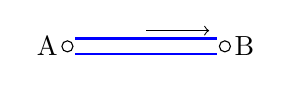
\begin{tikzpicture}
\draw (0,0) circle (2pt) node[left] {A};
\draw (2,0) circle (2pt) node[right] {B};
\draw[blue,thick] (0.1,0.1) -- (1.9,0.1);
\draw[blue,thick] (0.1,-0.1) -- (1.9,-0.1);
\draw[->] (1,0.2) -- (1.8,0.2);
\end{tikzpicture}
\caption{Pheromone trails and path selection}
\label{fig:aco_path}
\end{marginfigure}

\subsection{Differential Evolution (DE) Algorithm}
A vector-based evolutionary optimization algorithm. Provides effective results in continuous optimization problems.

\subsubsection{Basic Operators}
\begin{itemize}
    \item Mutation vector
    \item Crossover
    \item Selection
    \item Scaling factor (F)
    \item Crossover ratio (CR)
\end{itemize}

\begin{equation}
v_i = x_{r1} + F(x_{r2} - x_{r3})
\end{equation}

\begin{tcolorbox}[title=DE Strategies]
\begin{itemize}
    \item DE/rand/1/bin
    \item DE/best/1/bin
    \item DE/rand/2/bin
    \item DE/best/2/bin
    \item DE/current-to-best/1/bin
\end{itemize}
\end{tcolorbox}

\subsubsection{Algorithm Steps}
\begin{enumerate}
    \item Create initial population
    \item In each generation:
        \begin{itemize}
            \item Generate mutation vectors
            \item Apply crossover
            \item Perform selection
        \end{itemize}
    \item Continue until stopping criterion is met
\end{enumerate}

\sidenote{The differential evolution algorithm is particularly effective in continuous optimization problems. Parameter tuning is relatively easy and convergence speed is high.}

\subsection{Artificial Bee Colony (ABC) Optimization}
An optimization algorithm inspired by honey bees' food search behavior.

\subsubsection{Bee Types and Tasks}
\begin{itemize}
    \item Worker bees: Investigation of current resources
    \item Onlooker bees: Evaluation of promising resources
    \item Scout bees: Discovery of new resources
\end{itemize}

\begin{equation}
v_{ij} = x_{ij} + \phi_{ij}(x_{ij} - x_{kj})
\end{equation}

\begin{marginfigure}
\centering
\begin{tikzpicture}
\draw[->] (0,0) -- (4,0) node[right] {$x$};
\draw[->] (0,0) -- (0,4) node[above] {$f(x)$};
\filldraw[blue] (1,2) circle (2pt) node[above] {Worker};
\filldraw[red] (2,3) circle (2pt) node[above] {Onlooker};
\filldraw[green] (3,1) circle (2pt) node[above] {Scout};
\end{tikzpicture}
\caption{Role of different bee types in ABC}
\label{fig:abc_bees}
\end{marginfigure}

\subsubsection{Algorithm Steps}
\begin{enumerate}
    \item Determine initial food sources
    \item In each cycle:
        \begin{itemize}
            \item Worker bee phase
            \item Onlooker bee phase
            \item Scout bee phase
        \end{itemize}
    \item Continue until stopping criterion is met
\end{enumerate}

\subsection{Quantum and Hybrid Optimization Algorithms}
Approaches inspired by quantum mechanics principles and combining strengths of different algorithms.

\subsubsection{Quantum-Inspired Algorithms}
\begin{itemize}
    \item Quantum particle swarm
    \item Quantum genetic algorithm
    \item Quantum simulated annealing
\end{itemize}

\begin{equation}
\psi(x,t) = \frac{1}{\sqrt{2\pi\sigma^2}} e^{-\frac{(x-\mu)^2}{2\sigma^2}}
\end{equation}

\begin{tcolorbox}[title=Advantages of Quantum Mechanism]
\begin{itemize}
    \item Better exploration ability
    \item Avoiding local optima
    \item Fast convergence
    \item Utilizing uncertainty principle
\end{itemize}
\end{tcolorbox}

\subsection{Other Metaheuristic Optimization Algorithms}
Dozens of new metaheuristic optimization algorithms are added to the academic literature each year. Some of these algorithms can still present quite original approaches. However, within the basic classifications, many of them are developed by imitating certain mechanisms of previous algorithms to some extent. For an engineer looking at this topic from outside the academic perspective, understanding and being able to apply some basic algorithms is much more beneficial than constantly following new algorithms. Especially considering the development of artificial intelligence, what is really important is implementing theoretical knowledge in the right practical fields.   
\section{Ayrık Parametrelerin Optimizasyonu}
Ayrık (Discrete) değişkenler içeren optimizasyon problemlerinin çözüm yöntemleri bu bölümde incelenecektir. Özellikle yapısal sistemlerde karşılaşılan ayrık parametre optimizasyonu problemleri ve çözüm stratejileri ele alınacaktır.

\subsection{Ayrık ve Sürekli Optimizasyon Farkları}
Optimizasyon problemlerinin çözüm uzayı yapısına göre sınıflandırılması ve temel farklılıkların incelenmesi.

\subsubsection{Temel Farklılıklar}
\begin{itemize}
    \item Çözüm uzayının yapısı
    \item Kullanılabilecek yöntemler
    \item Hesaplama karmaşıklığı
    \item Gradyan bilgisinin kullanımı
\end{itemize}

\begin{tcolorbox}[title=Ayrık vs Sürekli Optimizasyon]
\begin{itemize}
    \item \textbf{Ayrık:}
        \begin{itemize}
            \item Kesikli çözüm uzayı
            \item Kombinatoryal yöntemler
            \item NP-zor problemler
            \item Gradyan kullanılamaz
        \end{itemize}
    \item \textbf{Sürekli:}
        \begin{itemize}
            \item Sürekli çözüm uzayı
            \item Gradyan tabanlı yöntemler
            \item Diferansiyellenebilirlik
            \item Lokal bilgi kullanımı
        \end{itemize}
\end{itemize}
\end{tcolorbox}

\subsection{Gezgin Satıcı Problemi (TSP)}
Ayrık optimizasyon problemlerinin klasik örneği olan TSP (Travelling Salesman Problem)\sidenote{
    
\qrcode[height=1in]{https://github.com/btayfur/structural-optimization/blob/main/Code/Examples/Exmp4}}, birçok gerçek dünya probleminin modellenmesinde kullanılır. Bu problem, bir satıcının belirli şehirleri en kısa mesafede dolaşması gerektiği senaryoyu ele alır. Her şehre yalnızca bir kez uğranması ve tur sonunda başlangıç noktasına dönülmesi gerekir. TSP, lojistik, üretim planlaması, PCB devre tasarımı ve DNA dizilimi gibi alanlarda uygulanır. Problemin çözüm uzayı, şehir sayısı arttıkça faktöriyel olarak büyüdüğünden (n şehir için n! olası tur), büyük ölçekli problemler için kesin çözüm bulmak hesaplama açısından oldukça zorludur.

\subsubsection{Problem Tanımı}
\begin{itemize}
    \item N şehir arasında en kısa turu bulma
    \item Her şehre bir kez uğrama
    \item Başlangıç noktasına dönme
    \item NP-zor problem sınıfı
\end{itemize}

\begin{equation}
\min \sum_{i=1}^n \sum_{j=1}^n d_{ij}x_{ij}
\end{equation}


\subsubsection{Çözüm Yaklaşımları}
\begin{itemize}
    \item Kesin yöntemler:
        \begin{itemize}
            \item Dal-sınır
            \item Tamsayılı programlama
        \end{itemize}
    \item Sezgisel yöntemler:
        \begin{itemize}
            \item En yakın komşu
            \item 2-opt, 3-opt
            \item Lin-Kernighan
        \end{itemize}
    \item Metasezgisel yöntemler:
        \begin{itemize}
            \item ACO
            \item GA
            \item Tabu arama
        \end{itemize}
\end{itemize}

\sidenote{TSP, ayrık optimizasyon problemlerinin prototip örneğidir. Birçok gerçek dünya problemi TSP'ye indirgenebilir. Ancak TSP için uygulanan her optimizasyon algoritması, bir başka problem için kullanılamayabilir. Dolayısıyla her optimizasyon problemi bazı yaygın problemlere benzese de, kendi özel yapısı gözönüne alınarak ele alınmalıdır.}

\subsection{Çelik Yapıların Kesit Optimizasyonu}
Ayrık optimizasyon problemlerinin, yapısal optimizasyonda en kolay karşılaşılacak örneği çelik yapıların kesit optimizasyonudur. Bu problemde, çelik yapılarda kullanılan standart kesitlerin seçimine dayalı bir optimizasyon problemi ele alınır.

\subsubsection{Problem Tanımı}
Çelik yapılarda kesit optimizasyonu, ayrık bir optimizasyon problemidir:
\begin{itemize}
    \item Standart kesit tabloları
    \item Yapısal kısıtlar
    \item Minimum ağırlık hedefi
    \item Gruplandırma gereksinimleri
\end{itemize}

\begin{equation}
\begin{aligned}
\min & \quad \sum_{i=1}^n \rho_i L_i A_i \\
\text{s.t.} & \quad \sigma_i \leq \sigma_{allow} \\
& \quad \delta \leq \delta_{allow} \\
& \quad A_i \in S
\end{aligned}
\end{equation}


\subsubsection{Çözüm Stratejileri}
\begin{itemize}
    \item Ayrık değişkenli optimizasyon
    \item Metasezgisel yöntemler
    \item Hibrit yaklaşımlar
    \item Paralel hesaplama
\end{itemize}

\begin{tcolorbox}[title=Optimizasyon Süreci]
\begin{enumerate}
    \item Yapısal analiz
    \item Kesit seçimi
    \item Kısıt kontrolü
    \item İteratif iyileştirme
\end{enumerate}
\end{tcolorbox}



\subsection{İndislerle Problem Çözümünün Basitleştirilmesi}
Çelik yapı optimizasyonu farklı biçimlerde ele alınabilir. Ancak eğer öntanımlı çelik kesitleri kullanıyorsa, kesit seçimi ayrık bir optimizasyon problemi olarak karşımıza çıkar. Bu durumda, kesit seçimi için bir veri yapısı oluşturmak ve bu veri yapısını kullanarak optimizasyon problemini çözmek gerekir. Bu noktada kesit listeleri indislenerek ele alınabilir. Ancak üzerine tartışılması gereken bir nokta şu olabilir: kesit listeleri hangi parametresi esas alınarak sıralanacak ve indislenecektir. Örneğin, yalnızca kesit alanının sıralamaya esas kabul edilmesi, eğilme mukavemeti açısından aynı sıralamanın oluşmasını garanti etmez. Fakat eğilme mukavemetinin esas alınması da aynı şekilde eksenel yük etkisi altında aynı sıralamanın oluşacağını garanti edemez. Dolayısıyla, problem özelinde kesit listelerinin farklı indisleme stratejisiyle ele alınması daha mantıklı olabilir. Örneğin, eksenel kuvvete maruz kalan elemanlarda kesit alanı esas alınırken, eğilme etkisin altındaki elemanlarda eğilme mukavemeti esas alınabilir. Veya daha etkili olacak farklı bir strateji geliştirebiliriz. 

\subsubsection{İndisleme Stratejisi}
\begin{itemize}
    \item Kesit grupları
    \item Eleman numaralandırma
    \item Düğüm noktaları
    \item Yükleme durumları
\end{itemize}

\begin{equation}
x_i = \text{ind}(A_i), \quad i = 1,\ldots,n
\end{equation}

\sidenote{İndisleme, ayrık optimizasyon problemlerinin çözümünü kolaylaştırır ve hesaplama verimliliğini artırır.}

\subsubsection{Veri Yapıları}
\begin{itemize}
    \item Kesit özellikleri tablosu
    \item Bağlantı matrisi
    \item Kısıt matrisi
    \item İndis dönüşüm tablosu
\end{itemize}

\begin{tcolorbox}[title=Veri Yapısı Örneği]
\begin{verbatim}
sections = {
    1: {'A': 10.3, 'I': 171},
    2: {'A': 13.2, 'I': 375},
    ...
}
\end{verbatim}
\end{tcolorbox}

\subsection{Optimizasyon Sonuçlarının Değerlendirilmesi}
Ayrık optimizasyon problemlerinin çözüm kalitesinin ve performansının analizi.

\subsubsection{Performans Ölçütleri}
\begin{itemize}
    \item Toplam ağırlık
    \item Maksimum gerilme oranı
    \item Maksimum deplasman
    \item Hesaplama süresi
\end{itemize}

\subsubsection{Sonuçların Görselleştirilmesi}
\begin{itemize}
    \item Yakınsama grafikleri
    \item Gerilme dağılımları
    \item Deplasman şekilleri
    \item Kesit dağılımları
\end{itemize}
  
\section{Sürekli Parametrelerin Optimizasyonu}
Sürekli parametrelerin optimizasyonuyla, yapısal mühendislikte ve diğer mühendislik alanlarında yaygın olarak karşılaşılır. Bu bölümde, sürekli değişkenlerle ifade edilen optimizasyon problemlerinin temel özellikleri, matematiksel formülasyonu ve çözüm yöntemleri incelenecektir.

\subsection{Sürekli Optimizasyonun Temel Kavramları}
Sürekli optimizasyon, tasarım değişkenlerinin sürekli değerler alabildiği optimizasyon problemlerini ifade eder. Bu tür problemlerde, tasarım uzayı sonsuz sayıda noktadan oluşur ve değişkenler herhangi bir reel değer alabilir.

\subsubsection{Sürekli Tasarım Değişkenleri}
Sürekli tasarım değişkenleri, belirli bir aralıkta herhangi bir değer alabilen parametrelerdir. Örneğin:
\begin{itemize}
    \item Bir kirişin kesit boyutları (genişlik, yükseklik)
    \item Malzeme özellikleri (elastisite modülü, yoğunluk)
    \item Geometrik parametreler (açılar, uzunluklar)
    \item Kontrol parametreleri (kuvvet büyüklükleri, sönümleme katsayıları)
\end{itemize}

\subsubsection{Sürekli Optimizasyon Problemlerinin Genel Formu}
Sürekli optimizasyon problemleri genellikle aşağıdaki formda ifade edilir:
\begin{align}
\min_{\mathbf{x}} \quad & f(\mathbf{x}) \\
\text{s.t.} \quad & g_i(\mathbf{x}) \leq 0, \quad i = 1, 2, \ldots, m \\
& h_j(\mathbf{x}) = 0, \quad j = 1, 2, \ldots, p \\
& \mathbf{x}_L \leq \mathbf{x} \leq \mathbf{x}_U
\end{align}

Burada:
\begin{itemize}
    \item $\mathbf{x} \in \mathbb{R}^n$ : Tasarım değişkenleri vektörü
    \item $f(\mathbf{x})$ : Amaç fonksiyonu
    \item $g_i(\mathbf{x})$ : Eşitsizlik kısıtları
    \item $h_j(\mathbf{x})$ : Eşitlik kısıtları
    \item $\mathbf{x}_L, \mathbf{x}_U$ : Alt ve üst sınırlar
\end{itemize}

\begin{tcolorbox}[title=Sürekli Optimizasyon Örneği]
Bir konsol kirişin ağırlık minimizasyonu problemi:
\begin{align}
\min_{b,h} \quad & \rho \cdot L \cdot b \cdot h \\
\text{s.t.} \quad & \sigma_{max} = \frac{6PL}{bh^2} \leq \sigma_{allow} \\
& \delta_{max} = \frac{PL^3}{3EI} \leq \delta_{allow} \\
& b_{min} \leq b \leq b_{max} \\
& h_{min} \leq h \leq h_{max}
\end{align}

Burada $b$ ve $h$ sırasıyla kirişin genişliği ve yüksekliğidir.
\end{tcolorbox}

\sidenote{Sürekli optimizasyon problemlerinde, amaç fonksiyonu ve kısıtlar genellikle sürekli ve türevlenebilir fonksiyonlardır, bu da gradyan tabanlı optimizasyon yöntemlerinin kullanılmasına olanak sağlar.}


\subsection{Sürekli Optimizasyon Problemlerinin Matematiksel Formülasyonu}

Sürekli optimizasyon problemlerinin matematiksel formülasyonu, problemin doğasını ve çözüm yöntemlerini belirleyen temel bir adımdır. Bu formülasyon, amaç fonksiyonu, kısıtlar ve tasarım değişkenlerinin matematiksel olarak ifade edilmesini içerir.

\subsubsection{Amaç Fonksiyonu}
Amaç fonksiyonu, optimize edilmek istenen mühendislik performans ölçütünü matematiksel olarak ifade eder. Yapısal optimizasyon problemlerinde yaygın olarak kullanılan amaç fonksiyonları şunlardır:

\begin{itemize}
    \item \textbf{Ağırlık minimizasyonu:} $f(\mathbf{x}) = \sum_{i=1}^{n} \rho_i V_i(\mathbf{x})$
    \item \textbf{Esneklik minimizasyonu:} $f(\mathbf{x}) = \mathbf{F}^T \mathbf{u}(\mathbf{x})$
    \item \textbf{Gerilme minimizasyonu:} $f(\mathbf{x}) = \max_{i} \sigma_i(\mathbf{x})$
    \item \textbf{Deplasman minimizasyonu:} $f(\mathbf{x}) = \max_{i} |u_i(\mathbf{x})|$
    \item \textbf{Frekans maksimizasyonu:} $f(\mathbf{x}) = -\omega_1(\mathbf{x})$ (ilk doğal frekans)
    \item \textbf{Maliyet minimizasyonu:} $f(\mathbf{x}) = \sum_{i=1}^{n} c_i x_i$
\end{itemize}

\subsubsection{Kısıt Fonksiyonları}
Kısıt fonksiyonları, tasarımın belirli gereksinimleri karşılamasını sağlayan matematiksel ifadelerdir. Yapısal optimizasyon problemlerinde sıklıkla kullanılan kısıtlar şunlardır:

\begin{itemize}
    \item \textbf{Gerilme kısıtları:} $g_i(\mathbf{x}) = \sigma_i(\mathbf{x}) - \sigma_{allow} \leq 0$
    \item \textbf{Deplasman kısıtları:} $g_i(\mathbf{x}) = |u_i(\mathbf{x})| - u_{allow} \leq 0$
    \item \textbf{Burkulma kısıtları:} $g_i(\mathbf{x}) = P_{cr,i}(\mathbf{x}) - P_{applied} \leq 0$
    \item \textbf{Frekans kısıtları:} $g_i(\mathbf{x}) = \omega_{min} - \omega_i(\mathbf{x}) \leq 0$
    \item \textbf{Denge kısıtları:} Yapının statik denge koşullarını sağlaması gerektiğini ifade eder.
    \item \textbf{Geometrik kısıtlar:} Tasarım değişkenlerinin belirli geometrik ilişkileri sağlaması gerektiğini ifade eder.
\end{itemize}

\subsubsection{Duyarlılık Analizi}
Duyarlılık analizi, amaç fonksiyonu ve kısıtların tasarım değişkenlerine göre türevlerinin hesaplanmasını içerir. Bu türevler, gradyan tabanlı optimizasyon algoritmalarında arama yönünü belirlemek için kullanılır.

\begin{equation}
\nabla f(\mathbf{x}) = \left[ \frac{\partial f}{\partial x_1}, \frac{\partial f}{\partial x_2}, \ldots, \frac{\partial f}{\partial x_n} \right]^T
\end{equation}

\begin{equation}
\nabla g_i(\mathbf{x}) = \left[ \frac{\partial g_i}{\partial x_1}, \frac{\partial g_i}{\partial x_2}, \ldots, \frac{\partial g_i}{\partial x_n} \right]^T
\end{equation}

Duyarlılık analizi için kullanılan yöntemler:
\begin{itemize}
    \item \textbf{Analitik yöntemler:} Türevlerin doğrudan matematiksel ifadelerle hesaplanması
    \item \textbf{Sonlu farklar yöntemi:} Nümerik yaklaşımla türevlerin hesaplanması
    \item \textbf{Adjoint yöntem:} Karmaşık sistemlerde verimli duyarlılık hesaplaması için kullanılır
    \item \textbf{Otomatik türev alma:} Bilgisayar programlarının otomatik olarak türev hesaplaması
\end{itemize}

\subsubsection{Sürekli Optimizasyonun Ayırt Edici Özellikleri}
Sürekli optimizasyon problemleri, ayrık optimizasyon problemlerinden farklı olarak, tasarım değişkenlerinin sürekli değerler alabildiği problemlerdir. Bu tür problemlerin ayırt edici özellikleri şunlardır:

\begin{itemize}
    \item \textbf{Sürekli tasarım uzayı:} Tasarım değişkenleri reel sayılar kümesinden değerler alabilir, bu da sonsuz sayıda olası çözüm anlamına gelir.
    
    \item \textbf{Türevlenebilirlik:} Amaç fonksiyonu ve kısıtlar genellikle türevlenebilir fonksiyonlardır, bu da gradyan tabanlı optimizasyon yöntemlerinin kullanılabilmesini sağlar.
    
    \item \textbf{Konvekslik:} Problem formülasyonunun konveks olup olmaması, global optimuma ulaşılabilirliği belirler. Konveks problemlerde, lokal optimum aynı zamanda global optimumdur.
    
    \item \textbf{Süreklilik:} Fonksiyonların sürekli olması, optimizasyon algoritmasının daha kararlı çalışmasını sağlar.
    
    \item \textbf{Diferansiyellenebilirlik:} Yüksek dereceden türevlerin varlığı, Newton benzeri yöntemlerin kullanılabilmesine olanak tanır.
\end{itemize}

Sürekli optimizasyon problemleri, yapısal mühendislikte kesit boyutları, malzeme özellikleri veya geometrik parametreler gibi değişkenlerin optimize edilmesinde yaygın olarak kullanılır. Bu problemlerin çözümünde, gradyan tabanlı yöntemler (Newton yöntemi, eşlenik gradyan yöntemi), gradyan gerektirmeyen yöntemler (Nelder-Mead simpleks yöntemi) veya meta-sezgisel algoritmalar (genetik algoritma, parçacık sürü optimizasyonu) kullanılabilir.

\subsection{Sürekli Optimizasyonun Yapısal Optimizasyondaki Genel Uygulamaları}
Bu noktada yaygın iki optimizasyon problemi örneklendirilmiş olsa da, parametrelere bağlı olarak hesaplanan birçok çıktı optimizasyon problemi olarak ele alınabilir ve iyileştirilebilir.

\subsubsection{Öntanımlı Olmayan Boyut Optimizasyonu}
Öntanımlı olmayan boyut optimizasyonu, yapısal elemanların kesit boyutlarının standart katalog değerleriyle sınırlı olmadan, sürekli değişkenler olarak ele alınmasını içerir. Bu yaklaşım, tasarımcılara daha geniş bir tasarım uzayı sunar ve potansiyel olarak daha verimli yapılar elde edilmesini sağlar. Geleneksel yaklaşımlarda, yapı elemanları için belirli standart kesitler (örneğin, I-profiller, kutu profiller) arasından seçim yapılırken, öntanımlı olmayan optimizasyonda kesit özellikleri (alan, atalet momenti, vb.) doğrudan tasarım değişkenleri olarak kullanılır.

Bu tür optimizasyon problemlerinde, genellikle minimum ağırlık veya maksimum rijitlik gibi amaçlar gözetilirken, gerilme, deplasman ve burkulma gibi yapısal kısıtlar dikkate alınır. Optimizasyon sonucunda elde edilen kesit özellikleri, daha sonra üretilebilir kesitlere dönüştürülmek üzere yorumlanır veya özel kesitler olarak üretilir. Öntanımlı olmayan boyut optimizasyonu, özellikle havacılık, uzay ve otomotiv endüstrilerinde, malzeme kullanımını minimize ederken performansı maksimize etmek için yaygın olarak kullanılmaktadır.


\subsubsection{Topolojik Optimizasyon}
Topolojik optimizasyon, bir yapının en verimli malzeme dağılımını belirlemek için kullanılan ileri bir yapısal optimizasyon yöntemidir. Bu yöntem, belirli bir tasarım alanı içinde malzemenin nerede bulunması ve nerede bulunmaması gerektiğine karar vererek, yapının temel formunu ve bağlantı yapısını optimize eder. Geleneksel optimizasyon yöntemlerinden farklı olarak, sadece boyutları veya şekli değil, yapının topolojisini de değiştirebilir.

Topolojik optimizasyon süreci genellikle bir tasarım alanının sonlu elemanlara bölünmesiyle başlar ve her elemana malzeme yoğunluğunu temsil eden bir tasarım değişkeni atanır. Optimizasyon algoritması, belirli kısıtlar altında (örneğin maksimum ağırlık veya minimum esneklik) bu değişkenleri ayarlayarak en iyi malzeme dağılımını arar. Sonuç olarak, genellikle doğada bulunan yapılara benzeyen, yüksek verimli ve hafif yapılar ortaya çıkar. Bu yöntem, otomotiv ve havacılık endüstrilerinde hafif parçalar tasarlamak, medikal implantlar geliştirmek ve 3D baskı teknolojileri için optimize edilmiş yapılar oluşturmak gibi çeşitli alanlarda yaygın olarak kullanılmaktadır.
  
\section{Yapısal Optimizasyona Giriş}
Yapısal optimizasyon, her ne kadar farklı bir optimizasyon türü olarak ele alınmış olsa da özü itibariyle tüm optimizasyon problemleriyle benzer prensiperle ilerler. Ancak problemin tanımlanması, dolayısıyla da efektif çözüm algoritmalarının seçilebilmesi mühendis yargısına bağlıdır. Bu bölümde klasik optimizasyon başlıkları altında tanımlanan kavramların yapısal optimizasyon bağlamında nasıl bir bağlama dönüştüğü anlatılmaya çalışılacaktır.

\subsection{Yapısal Optimizasyon Terminolojisi}

\subsubsection{Amaç Fonksiyonları}
Yapısal optimizasyonda amaç fonksiyonu, optimize edilmek istenen mühendislik hedefini matematiksel olarak ifade eder. Yapısal tasarımda en yaygın kullanılan amaç fonksiyonları şunlardır:\sidenote{Çok amaçlı optimizasyon problemlerinde, birden fazla amaç fonksiyonu ağırlıklandırılarak tek bir fonksiyona dönüştürülebilir veya Pareto-optimal çözümler aranabilir.}

\begin{itemize}
    \item \textbf{Ağırlık minimizasyonu:} Yapının toplam ağırlığını en aza indirmeyi hedefler. Özellikle havacılık ve uzay yapılarında kritik öneme sahiptir.
    \item \textbf{Maliyet minimizasyonu:} Yapının üretim, malzeme ve işçilik maliyetlerini en aza indirmeyi amaçlar.
    \item \textbf{Rijitlik maksimizasyonu:} Yapının belirli yükler altında deformasyona karşı direncini en üst düzeye çıkarmayı hedefler.
    \item \textbf{Dayanım maksimizasyonu:} Yapının taşıyabileceği maksimum yükü artırmayı amaçlar.
    \item \textbf{Enerji sönümleme:} Dinamik yükler altında yapının enerji sönümleme kapasitesini optimize eder.
\end{itemize}

\subsubsection{Kısıtlar}
Yapısal optimizasyonda kısıtlar, tasarımın uygulanabilir olması için sağlanması gereken şartları tanımlar. Bu kısıtlar, klasik optimizasyon problemlerindeki matematiksel kısıtların yapısal mühendislik bağlamındaki karşılıklarıdır:

\begin{itemize}
    \item \textbf{Gerilme kısıtları:} Yapıdaki gerilmelerin izin verilen maksimum değerleri aşmamasını sağlar. Örneğin: $\sigma_i \leq \sigma_{izin}$
    
    \item \textbf{Deplasman kısıtları:} Yapıdaki yer değiştirmelerin belirli sınırlar içinde kalmasını sağlar. Örneğin: $\delta_i \leq \delta_{izin}$
    
    \item \textbf{Burkulma kısıtları:} Yapı elemanlarının burkulma yüklerinin, uygulanan yüklerden belirli bir güvenlik faktörü kadar büyük olmasını sağlar.
    
    \item \textbf{Titreşim kısıtları:} Yapının doğal frekanslarının belirli değerlerin üzerinde veya altında olmasını sağlar.
    
    \item \textbf{Geometrik kısıtlar:} Yapısal optimizasyon bağlamında, tasarım değişkenlerinin fiziksel olarak uygulanabilir sınırlar içinde kalmasını sağlar. Örneğin:
    \begin{itemize}
        \item Minimum ve maksimum kesit boyutları
        \item Minimum duvar kalınlıkları
        \item Elemanlar arası bağlantı gereksinimleri\sidenote{Örneğin çelik bir yapının üst katlarında kullanılan kesit boyutları, alt katlarındaki kesit boyutlarından daha büyük olması istenebilir ve bu aplikasyon açısından da oldukça mantıklıdır.}
        \item Montaj ve üretim kısıtlamaları
    \end{itemize}
    
    \item \textbf{Denge kısıtları:} Yapının statik denge koşullarını sağlaması gerektiğini ifade eder.
    
    \item \textbf{Uyumluluk kısıtları:} Deformasyonların sürekli ve uyumlu olması gerektiğini belirtir.
\end{itemize}

\begin{tcolorbox}[title=Yapısal Optimizasyon Kısıtları Örneği]
Bir köprü tasarımında:
\begin{align}
\sigma_{max} &\leq 250 \text{ MPa} \quad \text{(Gerilme kısıtı)} \\
\delta_{orta} &\leq L/400 \quad \text{(Deplasman kısıtı)} \\
f_1 &\geq 2.0 \text{ Hz} \quad \text{(Titreşim kısıtı)} \\
t_{min} &\geq 8 \text{ mm} \quad \text{(Geometrik kısıt)}
\end{align}
\end{tcolorbox}

\sidenote{Kısıtların matematiksel formülasyonu, sonlu eleman analizinin sonuçlarına dayalı olarak ifade edilir ve genellikle doğrusal olmayan fonksiyonlar şeklindedir.}

\subsubsection{Tasarım Değişkenleri}
Yapısal optimizasyonda tasarım değişkenleri, optimize edilecek parametreleri temsil eder. Bu değişkenler, optimizasyon algoritması tarafından değiştirilebilen ve en iyi çözümü bulmak için ayarlanabilen parametrelerdir. Yapısal mühendislikte yaygın kullanılan tasarım değişkenleri şunlardır:

\begin{itemize}
    \item \textbf{Kesit özellikleri:} 
    \begin{itemize}
        \item Profil boyutları (genişlik, yükseklik)
        \item Duvar kalınlıkları
        \item Kesit alanı
        \item Atalet momenti
    \end{itemize}
    
    \item \textbf{Malzeme özellikleri:} 
    \begin{itemize}
        \item Elastisite modülü
        \item Yoğunluk
        \item Akma dayanımı
    \end{itemize}
    
    \item \textbf{Geometrik parametreler:} 
    \begin{itemize}
        \item Düğüm noktalarının koordinatları
        \item Eğrilik yarıçapları
        \item Açılar
    \end{itemize}
    
    \item \textbf{Topolojik parametreler:} 
    \begin{itemize}
        \item Malzeme varlığı/yokluğu (0-1 değişkenleri)
        \item Malzeme yoğunluğu (0-1 arasında değişen sürekli değişkenler)\sidenote{Optimizasyon veya regresyon benzeri birçok kodlama gerektiren hesaplama yönteminde, verilerin daha standart şekilde ele alınabilmesi için normalizasyon adlı bir yaklaşım kullanılır. Bu yaklaşım, verilerin 0-1 arasında değişen bir değer aralığına sahip olmasını sağlar. Mevcut veriler içerisindeki en küçük veri 0, en büyük veri ise 1 olarak dönüştürülür. Tüm ara değerler ise bu aralıkta oransal bir değer alır.}
        \item Bağlantı noktalarının varlığı
    \end{itemize}
\end{itemize}

\begin{tcolorbox}[title=Tasarım Değişkenleri Gösterimi]
Tipik bir çelik çerçeve optimizasyonunda tasarım değişkenleri şu şekilde gösterilebilir:
\begin{align}
\mathbf{x} = [A_1, A_2, \ldots, A_n, I_{y1}, I_{y2}, \ldots, I_{yn}, I_{z1}, I_{z2}, \ldots, I_{zn}]^T
\end{align}
Burada $A_i$ kesit alanlarını, $I_{yi}$ ve $I_{zi}$ ise atalet momentlerini temsil eder.
\end{tcolorbox}

\subsection{Yapısal Optimizasyon Kategorileri}

Yapısal optimizasyon problemleri kategorik olarak (Şekil, boyut, topoloji vb.) gibi bazı temel başlıklara ayrılabilir. Ancak bir mühendis, birbiriyle çelişen çıktıları üreten parametrelerin olduğu her sorunu bir optimizasyon problemi olarak ele alabilir. 

Örneğin bir yapıyı hafifletmek çoğu zaman gerilme kapasitelerinden feragat etmek anlamına gelebilir. Bu çelişen çıktılar, aynı parametrelerin sonucudur.

\subsubsection{Boyutlandırma Optimizasyonu}
Boyutlandırma optimizasyonu, yapının genel geometrisi sabit tutularak elemanların kesit boyutlarının optimize edilmesidir. En temel ve yaygın kullanılan yapısal optimizasyon yaklaşımıdır.

\begin{itemize}
    \item \textbf{Tasarım değişkenleri:} Kesit alanı, kalınlık, genişlik-yükseklik gibi kesit özellikleri
    \item \textbf{Avantajları:} 
    \begin{itemize}
        \item Matematiksel olarak nispeten daha basit formülasyon
        \item Mevcut tasarımların iyileştirilmesi için uygun
        \item Endüstride yaygın kullanım
    \end{itemize}
    \item \textbf{Uygulama alanları:} Çelik yapılar, çerçeve sistemler, kafes sistemler
\end{itemize}


\subsubsection{Şekil Optimizasyonu}
Şekil optimizasyonu, yapı elemanlarının şekillerinin veya düğüm noktalarının konumlarının değiştirilmesiyle gerçekleştirilir. Yapının genel topolojisi korunurken sınır geometrisi değiştirilir.

\begin{itemize}
    \item \textbf{Tasarım değişkenleri:} Düğüm noktalarının koordinatları, eğrilik parametreleri, kontrol noktaları
    \item \textbf{Avantajları:} 
    \begin{itemize}
        \item Boyutlandırma optimizasyonuna göre daha fazla tasarım esnekliği
        \item Gerilme yoğunlaşmalarının azaltılmasında etkili
    \end{itemize}
    \item \textbf{Zorluklar:} 
    \begin{itemize}
        \item Geometrik değişimler sonlu eleman ağının yeniden oluşturulmasını gerektirebilir
        \item Karmaşık matematiksel formülasyon
    \end{itemize}
    \item \textbf{Uygulama alanları:} Havacılık yapıları, otomotiv parçaları, köprü konstrüksiyonları
\end{itemize}

\subsubsection{Topoloji Optimizasyonu}
Topoloji optimizasyonu, yapının temel yapısının veya topolojisinin değiştirilmesiyle gerçekleştirilir. Malzemenin yapı içindeki dağılımı optimize edilir ve genellikle malzemenin olması veya olmaması gereken bölgeler belirlenir.

\begin{itemize}
    \item \textbf{Tasarım değişkenleri:} Malzeme yoğunluğu, malzeme varlığı/yokluğu
    \item \textbf{Avantajları:} 
    \begin{itemize}
        \item En yüksek tasarım serbestliği
        \item Yenilikçi ve öngörülemeyen tasarımlar üretebilme
        \item Malzeme kullanımında önemli tasarruf potansiyeli
    \end{itemize}
    \item \textbf{Zorluklar:} 
    \begin{itemize}
        \item Matematiksel ve hesaplamalı olarak karmaşık
        \item Üretilebilirlik kısıtlarının uygulanması zor olabilir
        \item Sonuçların yorumlanması ve uygulanabilir tasarımlara dönüştürülmesi
    \end{itemize}
    \item \textbf{Uygulama alanları:} Havacılık, otomotiv, medikal implantlar, 3D baskı yapıları
\end{itemize}


\begin{tcolorbox}[title=Örnek: Konsol Kiriş Optimizasyonu]
Aynı konsol kiriş probleminin üç farklı yaklaşımla optimizasyonu:

\textbf{Boyutlandırma:} Kiriş kesitinin yüksekliğinin uzunluk boyunca değişimi optimize edilir.

\textbf{Şekil:} Kirişin alt ve üst yüzeylerinin şekli optimize edilir.

\textbf{Topoloji:} Kirişin iç yapısındaki malzeme dağılımı optimize edilir, sonuçta genellikle kafes benzeri bir yapı ortaya çıkar.
\end{tcolorbox}

\subsection{Yapısal Optimizasyon Formülasyonu}

Bir yapısal optimizasyon problemi, matematiksel olarak şu şekilde ifade edilebilir:

\begin{align}
\text{Minimize: } & f(\mathbf{x}) \\
\text{Kısıtlar: } & g_j(\mathbf{x}) \leq 0, \quad j = 1, 2, \ldots, m \\
& h_k(\mathbf{x}) = 0, \quad k = 1, 2, \ldots, p \\
& \mathbf{x}_L \leq \mathbf{x} \leq \mathbf{x}_U
\end{align}

Burada:
\begin{itemize}
    \item $\mathbf{x}$ : tasarım değişkenleri vektörü
    \item $f(\mathbf{x})$ : amaç fonksiyonu (minimizasyon problemi için)
    \item $g_j(\mathbf{x})$ : eşitsizlik kısıtları
    \item $h_k(\mathbf{x})$ : eşitlik kısıtları
    \item $\mathbf{x}_L$ ve $\mathbf{x}_U$ : tasarım değişkenlerinin alt ve üst sınırları
\end{itemize}

\subsubsection{Sonlu Eleman Analizi ile Bağlantı}
Yapısal optimizasyon problemlerinde, amaç fonksiyonu ve kısıtlar genellikle sonlu eleman analizi (FEA) sonuçlarına bağlıdır. Bu bağlantı aşağıdaki şekilde ifade edilebilir:

\begin{align}
\mathbf{K}(\mathbf{x}) \mathbf{u} &= \mathbf{F} \\
f(\mathbf{x}) &= f(\mathbf{x}, \mathbf{u}(\mathbf{x})) \\
g_j(\mathbf{x}) &= g_j(\mathbf{x}, \mathbf{u}(\mathbf{x})) \\
h_k(\mathbf{x}) &= h_k(\mathbf{x}, \mathbf{u}(\mathbf{x}))
\end{align}

Burada:
\begin{itemize}
    \item $\mathbf{K}(\mathbf{x})$ : tasarım değişkenlerine bağlı rijitlik matrisi
    \item $\mathbf{u}$ : deplasman vektörü
    \item $\mathbf{F}$ : dış kuvvet vektörü
\end{itemize}

\begin{tcolorbox}[title=Yapısal Optimizasyon Algoritması Seçimi]
Yapısal optimizasyon problemlerinde algoritma seçimi şu faktörlere bağlıdır:
\begin{itemize}
    \item Problem boyutu (tasarım değişkeni sayısı)
    \item Kısıt sayısı ve karmaşıklığı
    \item Fonksiyon değerlendirmelerinin hesaplama maliyeti
    \item Tasarım uzayının karakteristiği (çoklu yerel optimumların varlığı)
    \item Duyarlılık bilgisinin mevcudiyeti
\end{itemize}
\end{tcolorbox}



  
\section{Topolojik Optimizasyon}
Yapısal sistemlerin en temel formunu belirlemeyi amaçlayan topolojik optimizasyon yöntemleri bu bölümde incelenecektir. Malzeme dağılımının optimizasyonu ve modern topoloji optimizasyonu teknikleri ele alınacaktır.

\subsection{Topolojik Optimizasyonun Temelleri}
Topolojik optimizasyon, bir yapının en verimli malzeme dağılımını belirlemek için kullanılan ileri bir yapısal optimizasyon yöntemidir. Geleneksel optimizasyon yöntemlerinden farklı olarak, topolojik optimizasyon sadece boyutları veya şekli değil, yapının temel formunu ve bağlantı yapısını da optimize eder. Bu yaklaşımda, belirli bir tasarım alanı içinde malzemenin nerede bulunması ve nerede bulunmaması gerektiğine karar verilir.

Topolojik optimizasyon süreci genellikle bir tasarım alanının sonlu elemanlara bölünmesiyle başlar. Her elemana, malzeme yoğunluğunu temsil eden 0 ile 1 arasında değişen bir tasarım değişkeni atanır. Optimizasyon algoritması, belirli kısıtlar altında (örneğin, maksimum ağırlık veya minimum esneklik) bu değişkenleri ayarlayarak en iyi malzeme dağılımını arar. Sonuç olarak, genellikle doğada bulunan yapılara benzeyen, yüksek verimli ve hafif yapılar ortaya çıkar.

Bu yöntem, otomotiv ve havacılık endüstrilerinde hafif ve dayanıklı parçalar tasarlamak, medikal implantlar geliştirmek ve 3D baskı teknolojileri için optimize edilmiş yapılar oluşturmak gibi çeşitli alanlarda yaygın olarak kullanılmaktadır. Topolojik optimizasyon, mühendislere geleneksel tasarım yaklaşımlarıyla elde edilmesi zor olan yenilikçi ve verimli çözümler sunma imkanı sağlar.


\subsubsection{Temel Kavramlar}
\begin{itemize}
    \item Malzeme dağılımı \sidenote{Tasarım alanı içinde malzemenin nasıl yerleştirildiğini gösteren, genellikle yoğunluk değişkenleriyle ifade edilen dağılım.}
    \item Yapısal topoloji \sidenote{Bir yapının temel formunu, bağlantı yapısını ve malzeme dağılımını tanımlayan geometrik düzen.}
    \item Homojenizasyon \sidenote{Mikro yapıların makro özelliklerini belirlemek için kullanılan, kompozit malzemelerin efektif özelliklerini hesaplama yöntemi.}
    \item Tasarım değişkenleri \sidenote{Optimizasyon sürecinde değiştirilebilen, genellikle her sonlu elemana atanan ve malzeme varlığını temsil eden parametreler.}
\end{itemize}

\begin{equation}
\min_{x \in [0,1]^n} \quad c(x) = F^T U(x)
\end{equation}

\subsection{Sonlu Elemanlar Yöntemi ve Optimizasyon İlişkisi}
Topolojik optimizasyon, sonlu elemanlar yöntemi (FEM) ile doğrudan ilişkilidir ve bu yöntem optimizasyon sürecinin temel bileşenidir. Sonlu elemanlar yöntemi, karmaşık geometrileri daha küçük ve basit elemanlara bölerek analiz etmeyi sağlar, bu da topolojik optimizasyon için gerekli olan yapısal davranışın hassas bir şekilde hesaplanmasına olanak tanır.

Optimizasyon sürecinde, her iterasyonda malzeme dağılımı değiştiğinde, yapının mekanik davranışı (gerilmeler, deplasmanlar, doğal frekanslar vb.) sonlu elemanlar analizi ile yeniden hesaplanır. Bu analiz sonuçları, optimizasyon algoritmasının bir sonraki adımda hangi bölgelerde malzeme ekleneceğine veya çıkarılacağına karar vermesini sağlar. Böylece FEM, topolojik optimizasyonun hem analiz hem de karar verme mekanizmasının ayrılmaz bir parçası haline gelir.

\subsubsection{FEM Formülasyonu}
\begin{itemize}
    \item Rijitlik matrisi
    \item Yük vektörü
    \item Deplasman alanı
    \item Eleman tipleri
\end{itemize}

\begin{equation}
K(x)U = F
\end{equation}

\subsubsection{Sonlu Eleman Modelinin API ile Oluşturulması}
Sonlu eleman modellerinin oluşturulması ve analizi için çeşitli yazılımlar Application Programming Interface (API) sunmaktadır. Bu API'ler, topolojik optimizasyon algoritmalarının sonlu eleman analizleriyle entegre çalışmasını sağlar. Özellikle otomatik iterasyon gerektiren optimizasyon süreçlerinde, API kullanımı manuel model oluşturma ve analiz süreçlerini ortadan kaldırarak büyük verimlilik sağlar.

SAP2000 OAPI (Open Application Programming Interface), yapısal analiz ve optimizasyon için yaygın kullanılan bir API örneğidir. Bu arayüz, Python, MATLAB veya C++ gibi programlama dilleri aracılığıyla SAP2000 yazılımının tüm özelliklerine erişim sağlar. Topolojik optimizasyon sürecinde, algoritma her iterasyonda SAP2000 OAPI kullanarak:

\begin{itemize}
    \item Güncellenmiş malzeme özelliklerini modele uygulayabilir
    \item Analizi otomatik olarak çalıştırabilir
    \item Analiz sonuçlarını (gerilmeler, deplasmanlar, vb.) okuyabilir
    \item Bu sonuçlara göre yeni malzeme dağılımını hesaplayabilir
\end{itemize}

Bu tür API entegrasyonları, topolojik optimizasyon sürecinin tamamen otomatikleştirilmesini sağlayarak, karmaşık yapıların bile verimli bir şekilde optimize edilmesine olanak tanır. Ayrıca ANSYS, Abaqus ve NASTRAN gibi diğer sonlu eleman yazılımları da benzer API'ler sunmaktadır. İlerleyen konularda SAP2000 OAPI'nin kullanıldığı daha detaylı örnekler incelenecektir.

\subsection{Yoğunluk Tabanlı Yöntemler}
Yoğunluk tabanlı topolojik optimizasyon yöntemlerinin en yaygın kullanılanı SIMP (Solid Isotropic Material with Penalization) yöntemidir. Bu yöntem, her sonlu elemana 0 ile 1 arasında değişen bir yoğunluk değişkeni atayarak çalışır. Burada 0 malzeme yokluğunu, 1 ise tam malzeme varlığını temsil eder.

SIMP yönteminin temel prensibi, ara yoğunluk değerlerini (0 ile 1 arasındaki değerler) cezalandırarak, optimizasyon sonucunda daha belirgin bir 0-1 dağılımı elde etmektir. Bu, malzeme özelliklerinin (örneğin elastisite modülü) yoğunluk değişkeninin bir üs fonksiyonu olarak tanımlanmasıyla sağlanır. Ceza parametresi genellikle 3 veya daha yüksek bir değer olarak seçilir.

SIMP yöntemi, otomotiv parçalarının hafifletilmesi, uçak yapısal elemanlarının optimizasyonu ve medikal implantların tasarımı gibi çeşitli mühendislik uygulamalarında başarıyla kullanılmaktadır. Yöntem, matematiksel olarak iyi tanımlanmış olması ve gradyan tabanlı optimizasyon algoritmaları ile uyumlu çalışması sayesinde endüstride standart bir yaklaşım haline gelmiştir.

\subsubsection{SIMP Yöntemi}
Solid Isotropic Material with Penalization:
\begin{equation}
E(x) = E_{min} + x^p(E_0 - E_{min})
\end{equation}

\begin{itemize}
    \item Yoğunluk değişkenleri: $x \in [0,1]$
    \item Ceza parametresi: $p > 1$
    \item Minimum rijitlik: $E_{min}$
    \item Tam malzeme rijitliği: $E_0$
\end{itemize}

\begin{tcolorbox}[title=SIMP Yönteminin Avantajları]
\begin{itemize}
    \item Basit implementasyon
    \item Hızlı yakınsama
    \item Ara yoğunlukların penalizasyonu
    \item Endüstriyel uygulamalarda yaygın kullanım
\end{itemize}
\end{tcolorbox}

\subsection{ESO ve BESO Yöntemleri}
Evolutionary Structural Optimization (ESO) ve Bi-directional Evolutionary Structural Optimization (BESO) yöntemleri, yapısal topoloji optimizasyonunda kullanılan sezgisel yaklaşımlardır. ESO yöntemi, "verimsiz malzemeyi kademeli olarak kaldır" prensibine dayanır ve düşük gerilme veya enerji yoğunluğuna sahip elemanları yapıdan çıkararak optimum tasarıma ulaşmayı hedefler. BESO ise ESO'nun geliştirilmiş bir versiyonudur ve sadece malzeme çıkarma değil, aynı zamanda gerekli bölgelere malzeme ekleme işlemini de içerir. Bu yöntemler, matematiksel olarak SIMP kadar sağlam bir temele sahip olmasa da, uygulanması kolay ve sezgisel olarak anlaşılabilir olmaları nedeniyle mühendislik uygulamalarında tercih edilmektedir.

\subsection{Level-Set Yöntemi}
Level-Set yöntemi, topoloji optimizasyonunda yapı sınırlarını açık bir şekilde tanımlamak için kullanılan matematiksel bir yaklaşımdır. Bu yöntemde, yapının sınırları bir seviye kümesi fonksiyonunun sıfır seviye eğrisi (veya yüzeyi) olarak temsil edilir. Optimizasyon süreci boyunca, bu seviye kümesi fonksiyonu Hamilton-Jacobi denklemleri kullanılarak güncellenir ve böylece yapı sınırları pürüzsüz bir şekilde evrilir. Level-Set yöntemi, keskin ve net sınırlar oluşturma, topoloji değişikliklerini doğal bir şekilde ele alma ve üretilebilirlik kısıtlarını kolayca dahil etme gibi avantajlara sahiptir. Özellikle akışkan-yapı etkileşimi problemleri ve çok malzemeli tasarımlarda etkili sonuçlar vermektedir.  
\section{Size and Shape Optimization}
The optimization of size and shape parameters of structural systems can also be called cross-section optimization in a more general sense. Depending on the problem, one or both of these can become parameters of the problem simultaneously.

\subsection{Foundations of Size Optimization}
Size optimization is an optimization method used to determine the optimal values of cross-sectional properties (width, height, thickness, etc.) of structural systems. This method aims to reach the optimum design by changing only the dimensions of elements without altering the topology of the structure.

\subsubsection{Problem Parameters}
Design variables used in size optimization typically include:
\begin{itemize}
    \item \textbf{Cross-section dimensions:} Width and height of beams, thickness of plates
    \item \textbf{Cross-sectional areas:} Cross-sectional areas of bar elements
    \item \textbf{Moments of inertia:} Parameters determining bending and torsional stiffness of beams
    \item \textbf{Material properties:} Variables such as elasticity modulus, density
    \item \textbf{Reinforcement elements:} Dimensions and locations of strengthening elements
\end{itemize}

\subsubsection{Problem Outputs}
The outputs obtained as a result of size optimization are:
\begin{itemize}
    \item \textbf{Optimum cross-section dimensions:} Most suitable dimensions for each structural element
    \item \textbf{Minimum weight/cost:} Total weight or cost of the structure obtained as a result of optimization
    \item \textbf{Structural performance indicators:} Stresses, displacements, natural frequencies
    \item \textbf{Material usage efficiency:} How efficiently the load-bearing capacity of each element is used
    \item \textbf{Sensitivity information:} Effects of changes in design variables on the objective function
\end{itemize}

\subsubsection{Constraints and Decision Mechanism}
In size optimization, various constraints limit the solution space and affect the decision mechanism:

\begin{itemize}
    \item \textbf{Stress constraints:} $\sigma_{max} \leq \sigma_{allow}$
    \begin{itemize}
        \item Maximum stresses in the structure must not exceed allowable values
        \item Affects in the direction of increasing element dimensions
    \end{itemize}
    
    \item \textbf{Displacement constraints:} $\delta_{max} \leq \delta_{allow}$
    \begin{itemize}
        \item Ensures maximum displacements in the structure remain within certain limits
        \item Generally affects in the direction of increasing structural stiffness
    \end{itemize}
    
    \item \textbf{Buckling constraints:} $P_{cr} \geq P_{design}$
    \begin{itemize}
        \item Ensures buckling loads of compression elements are greater than design load
        \item Affects in the direction of increasing dimensions of slender elements
    \end{itemize}
    
    \item \textbf{Frequency constraints:} $\omega_i \geq \omega_{min}$ or $\omega_i \leq \omega_{max}$
    \begin{itemize}
        \item Ensures natural frequencies of the structure are within certain ranges
        \item Important in structures subjected to dynamic loads
    \end{itemize}
    
    \item \textbf{Manufacturability constraints:} $x_{min} \leq x \leq x_{max}$
    \begin{itemize}
        \item Ensures design variables remain within practical manufacturing limits
        \item Limits solution space with realistic values
    \end{itemize}
    
    \item \textbf{Geometric constraints:} For example $h/b \leq \alpha$
    \begin{itemize}
        \item Ensures cross-section ratios remain within certain limits
        \item Prevents local buckling and stability issues
    \end{itemize}
\end{itemize}

\begin{tcolorbox}[title=Size Optimization Process]
\begin{enumerate}
    \item Creation of initial design
    \item Performance evaluation with structural analysis (FEM)
    \item Determination of effects of design variables through sensitivity analysis
    \item Updating design variables with optimization algorithm
    \item Repetition of steps 2-4 until convergence is achieved
\end{enumerate}
\end{tcolorbox}

Size optimization is widely used in structural engineering applications such as cross-section optimization of steel structures, reinforcement optimization of reinforced concrete structures, and bridge and tower design. As a result of optimization, while material usage is reduced, structural performance requirements are met, thus obtaining more economical and sustainable designs.

\subsection{Foundations of Shape Optimization}
The optimization of external boundaries and internal voids of structural elements can be approached in different ways depending on the engineer's perspective.

\begin{itemize}
    \item \textbf{Boundary Representation:} Geometric parameters
    \item \textbf{Control Points:} Shape change control
    \item \textbf{Smoothness:} Geometric continuity
\end{itemize}

\sidenote{Shape optimization improves the geometry of the structure without changing the topology.}

\subsection{Mathematical Formulation}
Mathematical expression of size and shape optimization problems:

\begin{equation}
\begin{aligned}
& \text{minimize} & & f(\mathbf{x}, \mathbf{s}) \\
& \text{subject to} & & g_i(\mathbf{x}, \mathbf{s}) \leq 0, & & i = 1,\ldots,m \\
& & & h_j(\mathbf{x}, \mathbf{s}) = 0, & & j = 1,\ldots,p \\
& & & \mathbf{x}^L \leq \mathbf{x} \leq \mathbf{x}^U \\
& & & \mathbf{s}^L \leq \mathbf{s} \leq \mathbf{s}^U
\end{aligned}
\end{equation}

Where:
\begin{itemize}
    \item \(\mathbf{x}\): Size parameters
    \item \(\mathbf{s}\): Shape parameters
    \item \(f\): Objective function
    \item \(g_i, h_j\): Constraint functions
\end{itemize}

\subsection{Parametric Modeling}
Mathematical representation of design variables:

\begin{itemize}
    \item \textbf{CAD Parameters:} Geometric dimensions
    \item \textbf{Spline Curves:} Boundary representation
    \item \textbf{Morph Box:} Shape deformation
\end{itemize}

\subsection{Sensitivity Analysis}
In some structural optimization problems, sensitivity analysis can be performed for design variables (parameters). However, since structural optimization problems are generally hyperstatic in nature, sensitivity analyses may not yield expected results and can even be misleading. \sidenote{The issue of hyperstaticity is important from an optimization perspective. For example, a cross-section chosen for one parameter, despite being close to the limit strength, can completely affect the load distribution due to changes in the cross-section of another parameter of the structure, causing the stress of the first cross-section to fall well below or exceed the limit strength.}

\subsection{Constraint Handling}
Handling of design constraints:

\begin{itemize}
    \item \textbf{Stress Constraints:} Material strength
    \item \textbf{Displacement Constraints:} Deformation limits
    \item \textbf{Geometric Constraints:} Manufacturability
\end{itemize}

\subsection{Multi-Objective Optimization}
Multi-objective optimization will be discussed in much more detail later.

\begin{tcolorbox}[title=Multi-Objective Approaches]
\begin{itemize}
    \item \textbf{Pareto Optimization:} Trade-off analysis
    \item \textbf{Weighted Sum:} Single objective function
    \item \textbf{Goal Programming:} Ideal point approach
\end{itemize}
\end{tcolorbox}

\subsection{Mesh Adaptation}
The mesh creation process, which can often turn into a nightmare in finite element models, can sometimes be the subject of optimization. However, this topic belongs to a separate field of expertise and course.

\begin{itemize}
    \item \textbf{Mesh Quality:} Element shape control
    \item \textbf{Adaptive Mesh:} Automatic mesh improvement
    \item \textbf{Remeshing:} Mesh regeneration
\end{itemize}

\subsection{Manufacturability and Practical Constraints}
Practical applicability of the design:

\begin{itemize}
    \item \textbf{Standard Sections:} Catalog selection
    \item \textbf{Manufacturing Method:} Production constraints
    \item \textbf{Cost:} Economic factors
\end{itemize}

\sidenote{Manufacturability constraints require balancing between theoretical optimum and practical solution, and this can be considered as a completely different optimization problem.}

\subsection{Evaluation of Optimization Results}
Analysis and interpretation of obtained results:

\begin{tcolorbox}[title=Evaluation Criteria]
\begin{itemize}
    \item \textbf{Performance Improvement:} Gains compared to initial state
    \item \textbf{Constraint Satisfaction:} Control of all design constraints
    \item \textbf{Manufacturability:} Analysis of practical applicability
    \item \textbf{Cost Analysis:} Economic evaluation
\end{itemize}
\end{tcolorbox}   
\section{Çok Amaçlı Optimizasyon}
Yapısal sistemlerin optimizasyonunda zaman zaman birbiriyle çelişen birden fazla amacın eş zamanlı olarak optimize edilmesi gerekebilir. Bu bölümde, çok amaçlı optimizasyon yöntemleri ve uygulamaları incelenecektir. \sidenote{Çok amaçlı optimizasyonda, tek bir optimal çözüm yerine Pareto-optimal çözümler kümesi elde edilir.
Çok amaçlı optimizasyonun daha iyi anlaşılması için bağlantıdaki örnek kod incelenebilir.


\qrcode[height=1in]{https://github.com/btayfur/structural-optimization/blob/main/Code/Examples/Exmp5/}}

\subsection{Çok Amaçlı Optimizasyonun Temelleri}
Birden fazla amaç fonksiyonunun eş zamanlı optimizasyonu:

\begin{tcolorbox}[title=Temel Kavramlar]
\begin{itemize}
    \item \textbf{Pareto Optimallik:} Baskın çözümler
    \item \textbf{Trade-off:} Amaçlar arası ödünleşim
    \item \textbf{Karar Verme:} Çözüm seçimi
    \item \textbf{Ağırlıklandırma:} Amaçların önceliklendirilmesi
\end{itemize}
\end{tcolorbox}

\subsection{Matematiksel Formülasyon}
Çok amaçlı optimizasyon probleminin genel yapısı:

\begin{equation}
\begin{aligned}
& \text{minimize} & & \mathbf{F}(\mathbf{x}) = [f_1(\mathbf{x}), f_2(\mathbf{x}), \ldots, f_k(\mathbf{x})]^T \\
& \text{subject to} & & g_i(\mathbf{x}) \leq 0, & & i = 1,\ldots,m \\
& & & h_j(\mathbf{x}) = 0, & & j = 1,\ldots,p \\
& & & \mathbf{x}^L \leq \mathbf{x} \leq \mathbf{x}^U
\end{aligned}
\end{equation}




\begin{marginfigure}
\centering
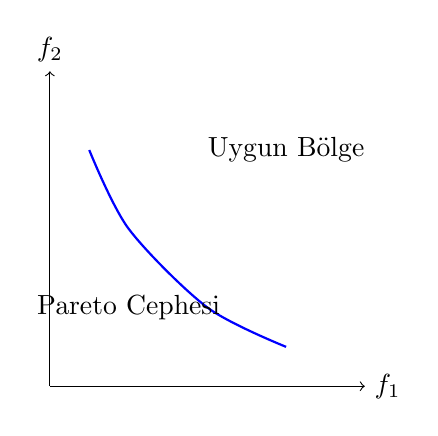
\begin{tikzpicture}
\draw[->] (0,0) -- (4,0) node[right] {$f_1$};
\draw[->] (0,0) -- (0,4) node[above] {$f_2$};
\draw[blue,thick] plot[smooth] coordinates {(0.5,3) (1,2) (2,1) (3,0.5)};
\node at (3,3) {Uygun Bölge};
\node at (1,1) {Pareto Cephesi};
\end{tikzpicture}
\caption{Pareto cephesi örneği}
\end{marginfigure}

\subsection{Çözüm Yaklaşımları}
Çok amaçlı optimizasyon problemlerinin çözümünde kullanılan temel stratejilerin incelenmesi, problemi ele alış biçimine göre farklı yaklaşımlar sunar. Yani esas olarak burada karar verici mühendisin kendisidir. Amaç fonksiyonlarının birbirlerine kıyasla üstün olup olmaması veya oransallığı bu kararda ve seçilecek stratejide etkilidir.

\subsubsection{Skalerleştirme Yöntemleri}
Çok amaçlı optimizasyon problemini tek amaçlı probleme dönüştüren yaklaşımlardır. Bu yöntemler, çoklu amaçları birleştirerek problemi daha kolay çözülebilir hale getirir. Skalerleştirme yöntemleri, hızlı ve kolay uygulanabilir olmaları nedeniyle mühendislik problemlerinde yaygın olarak kullanılır. Ancak uygun ağırlıkların belirlenmesi, çözümün kalitesini doğrudan etkilediği için süreci zorlaştırabilir.

\begin{tcolorbox}[title=Yaygın Skalerleştirme Yöntemleri]
\begin{itemize}
    \item \textbf{Ağırlıklı Toplam Yöntemi:} $F(x) = \sum_{i=1}^{k} w_i f_i(x)$
    \item \textbf{$\varepsilon$-Kısıt Yöntemi:} Bir amaç optimize edilirken diğerleri kısıt olarak tanımlanır
    \item \textbf{Hedef Programlama:} $\min \sum_{i=1}^{k} w_i |f_i(x) - T_i|$ (burada $T_i$ hedef değerlerdir)
\end{itemize}
\end{tcolorbox}

\subsubsection{Pareto Tabanlı Yaklaşımlar}
Pareto tabanlı yaklaşımlar, tüm Pareto-optimal çözümleri veya bunların iyi bir temsilini bulmayı hedefler. Bu yöntemler, çözüm uzayının daha geniş bir bölümünü keşfetmeyi sağlar ve karar vericiye daha fazla alternatif sunar. Pareto tabanlı yaklaşımlar, özellikle evrimsel algoritmaların kullanıldığı durumlarda daha etkilidir.

Pareto tabanlı yaklaşımların temel bileşenleri şunlardır:
\begin{itemize}
    \item \textbf{Baskınlık İlişkisi:} Bir çözümün diğerine göre daha iyi olup olmadığının belirlenmesi
    \item \textbf{Çeşitlilik Mekanizmaları:} Pareto cephesi boyunca çözümlerin homojen dağılmasını sağlayan teknikler
    \item \textbf{Elit Stratejiler:} İyi çözümlerin korunmasını sağlayan mekanizmalar
\end{itemize}

\begin{marginfigure}
\centering
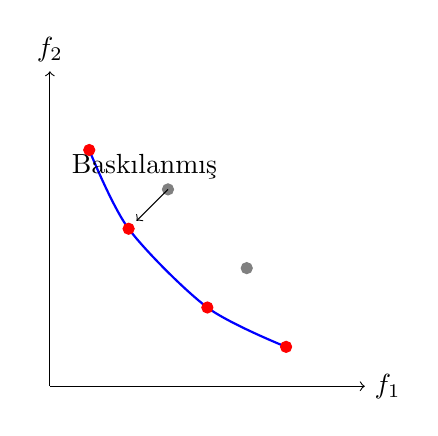
\begin{tikzpicture}
\draw[->] (0,0) -- (4,0) node[right] {$f_1$};
\draw[->] (0,0) -- (0,4) node[above] {$f_2$};
\draw[blue,thick] plot[smooth] coordinates {(0.5,3) (1,2) (2,1) (3,0.5)};
\filldraw[red] (0.5,3) circle (2pt);
\filldraw[red] (1,2) circle (2pt);
\filldraw[red] (2,1) circle (2pt);
\filldraw[red] (3,0.5) circle (2pt);
\filldraw[gray] (1.5,2.5) circle (2pt);
\filldraw[gray] (2.5,1.5) circle (2pt);
\draw[->] (1.5,2.5) -- (1.1,2.1);
\node at (1.2,2.8) {Baskılanmış};
\end{tikzpicture}
\caption{Pareto baskınlık kavramı}
\end{marginfigure}

\subsubsection{İnteraktif Yöntemler}
İnteraktif yöntemler, karar vericiyi optimizasyon sürecine dahil ederek, tercihlerine göre çözüm uzayını daraltır. Bu yaklaşım, karar vericinin bilgi ve deneyimini algoritmanın çalışmasına entegre eder. İnteraktif yöntemler, özellikle karmaşık mühendislik problemlerinde, uzman bilgisinin çözüm sürecine dahil edilmesi açısından değerlidir.

İnteraktif yaklaşımların avantajları:
\begin{itemize}
    \item Karar vericinin tercihlerini doğrudan sürece yansıtabilme
    \item Hesaplama kaynaklarını ilgi duyulan çözüm bölgesine yönlendirme
    \item Daha anlamlı ve uygulanabilir sonuçlar elde etme
\end{itemize}

\subsection{Evrimsel Çok Amaçlı Optimizasyon Algoritmaları}
Evrimsel algoritmaların çok amaçlı optimizasyon problemlerine uygulanması, klasik yöntemlere göre önemli avantajlar sağlar. Bu algoritmalar, tek seferde birden fazla çözüm üretebilme, karmaşık amaç fonksiyonlarını ele alabilme ve geniş çözüm uzaylarını etkili bir şekilde tarayabilme özellikleriyle öne çıkar.

\subsubsection{NSGA-II (Non-dominated Sorting Genetic Algorithm)}
NSGA-II, çok amaçlı evrimsel optimizasyon alanında en yaygın kullanılan algoritmalardan biridir. Baskınlık sıralama ve yoğunluk mesafesi hesaplama mekanizmalarıyla, hem Pareto-optimal çözümlere yakınsama hem de çözümler arasında çeşitlilik sağlar. NSGA-II, $O(MN^2)$ hesaplama karmaşıklığıyla oldukça verimli çalışır ve birçok mühendislik probleminde başarıyla uygulanmıştır.

NSGA-II'nin temel bileşenleri:
\begin{itemize}
    \item \textbf{Hızlı Baskınlık Sıralama:} Popülasyondaki çözümleri baskınlık ilişkisine göre sıralar
    \item \textbf{Yoğunluk Mesafesi:} Aynı baskınlık seviyesindeki çözümler arasında çeşitliliği korur
    \item \textbf{İkili Turnuva Seçimi:} Baskınlık seviyesi ve yoğunluk mesafesine dayalı seçim mekanizması
\end{itemize}


\subsubsection{MOEA/D (Multiobjective Evolutionary Algorithm based on Decomposition)}
MOEA/D, çok amaçlı optimizasyon problemini bir dizi tek amaçlı alt probleme ayrıştırarak çözen bir evrimsel algoritmadır. Her alt problem, komşu alt problemlerle bilgi paylaşımı yaparak eş zamanlı olarak optimize edilir. Bu yaklaşım, özellikle çok sayıda amaç fonksiyonu içeren problemlerde etkilidir ve hesaplama açısından verimlidir.

MOEA/D'nin avantajları:
\begin{itemize}
    \item Komşuluk yapısı sayesinde etkili bilgi paylaşımı
    \item Çok sayıda amaç fonksiyonu içeren problemlere uygunluk
    \item Farklı ayrıştırma yöntemlerinin kullanılabilmesi (Tchebycheff, ağırlıklı toplam vb.)
\end{itemize}

\subsubsection{SPEA2 (Strength Pareto Evolutionary Algorithm)}
SPEA2, sabit büyüklükte bir arşiv kullanarak Pareto-optimal çözümleri saklayan ve rafine eden bir evrimsel algoritmadır. Algoritma, her çözüme bir uygunluk değeri atayarak hem baskınlık ilişkisini hem de çözüm yoğunluğunu dikkate alır. SPEA2, özellikle çeşitlilik ve yakınsama arasında iyi bir denge kurması nedeniyle tercih edilir.

SPEA2'nin önemli özellikleri:
\begin{itemize}
    \item \textbf{Güç Değeri:} Bir çözümün kaç çözümü baskıladığını ölçer
    \item \textbf{Yoğunluk Tahmini:} K-en yakın komşu yöntemiyle hesaplanır
    \item \textbf{Harici Arşiv:} Pareto-optimal çözümleri etkin bir şekilde depolar ve günceller
\end{itemize}

\subsection{Karar Verme Süreçleri}
Çok amaçlı optimizasyon, bir dizi Pareto-optimal çözüm üretir ve bu çözümler arasından seçim yapılması gerekir. Karar verme süreci, optimizasyon sürecinin kritik bir parçasıdır ve çeşitli yaklaşımlarla desteklenebilir.

\subsubsection{Çözüm Seçimi Kriterleri}
Pareto-optimal çözümler arasından seçim yaparken kullanılabilecek çeşitli kriterler vardır:
\begin{itemize}
    \item \textbf{Uzaklık Ölçüleri:} İdeal noktaya en yakın çözüm (örn. Öklid mesafesi, Tchebycheff mesafesi)
    \item \textbf{Tatmin Düzeyi:} Her amaç için belirlenen eşik değerlerini sağlayan çözümler
    \item \textbf{Göreceli İyileştirme:} Bir amacın diğerine göre iyileşme oranı (trade-off analizi)
    \item \textbf{Risk Analizi:} Belirsizlik altında çözümlerin güvenilirliği
\end{itemize}

\begin{tcolorbox}[title=Örnek: Ağırlıklı Tchebycheff Metriği]
\begin{equation}
d(F, F^*) = \max_{i=1,...,k} \{w_i \cdot |F_i - F_i^*|\}
\end{equation}
Burada $F^*$ ideal nokta, $w_i$ amaçların ağırlıkları, $F_i$ mevcut çözümün $i$. amaç değeridir.
\end{tcolorbox}

\subsubsection{Ağırlıklandırma Stratejileri}
Amaçların göreceli önemini belirlemek için çeşitli ağırlıklandırma stratejileri kullanılabilir:
\begin{itemize}
    \item \textbf{Doğrudan Atama:} Karar vericinin doğrudan ağırlık ataması
    \item \textbf{AHP (Analitik Hiyerarşi Süreci):} İkili karşılaştırmalar yoluyla ağırlık belirleme
    \item \textbf{Entropi Tabanlı Yöntemler:} Veri dağılımına göre ağırlık hesaplama
    \item \textbf{TOPSIS:} İdeal çözüme benzerlik ile ağırlıklandırma
\end{itemize}

\subsubsection{Çözümler Arası Kıyaslama}
Farklı Pareto-optimal çözümlerin karşılaştırılması, karar vericinin tercihine uygun çözümü seçmesine yardımcı olur:
\begin{itemize}
    \item \textbf{Görselleştirme Teknikleri:} Paralel koordinat grafikleri, yıldız diyagramları, ısı haritaları
    \item \textbf{Duyarlılık Analizi:} Parametrelerdeki değişimlerin çözüme etkisi
    \item \textbf{Robust Değerlendirme:} Belirsizlik altında çözümlerin performansı
    \item \textbf{Yaşam Döngüsü Analizi:} Uzun vadeli performans ve maliyet değerlendirmesi
\end{itemize}

\begin{marginfigure}
\centering
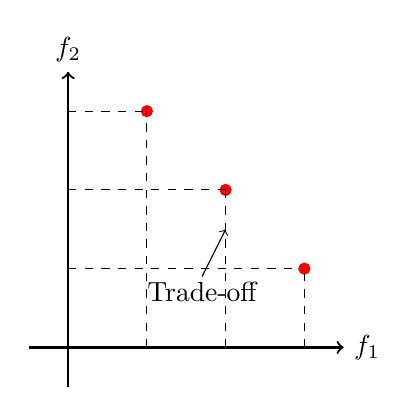
\begin{tikzpicture}
\draw[->,thick] (-0.5,0) -- (3.5,0) node[right] {$f_1$};
\draw[->,thick] (0,-0.5) -- (0,3.5) node[above] {$f_2$};
\filldraw[red] (1,3) circle (2pt);
\filldraw[red] (2,2) circle (2pt);
\filldraw[red] (3,1) circle (2pt);
\draw[dashed] (1,0) -- (1,3);
\draw[dashed] (0,3) -- (1,3);
\draw[dashed] (2,0) -- (2,2);
\draw[dashed] (0,2) -- (2,2);
\draw[dashed] (3,0) -- (3,1);
\draw[dashed] (0,1) -- (3,1);
\node at (1.7,0.7) {Trade-off};
\draw[->] (1.7,0.9) -- (2,1.5);
\end{tikzpicture}
\caption{Pareto çözümleri arasındaki trade-off analizi}
\end{marginfigure}


\subsection{Çok Amaçlı Optimizasyonda Performans Metrikleri}
\subsubsection{Hypervolume (Hiperhaciim)}
Hiperhacim, çok amaçlı optimizasyon algoritmalarının performansını değerlendirmek için kullanılan en yaygın metriklerden biridir. Bu metrik, Pareto cephesinin referans noktasına göre kapladığı alanın veya hacmin ölçüsünü ifade eder. Daha yüksek hiperhacim değeri, algoritmanın daha iyi bir Pareto cephesi bulduğunu gösterir, çünkü bu durum çözüm uzayının daha geniş bir bölümünün kapsandığını ifade eder.

\subsubsection{IGD (Ters Nesil Mesafesi)}
Ters Nesil Mesafesi (IGD), gerçek Pareto cephesi ile algoritma tarafından bulunan çözüm kümesi arasındaki mesafenin bir ölçüsüdür. Bu metrik, bulunan çözümlerin gerçek Pareto cephesine ne kadar yakın olduğunu ve cepheyi ne kadar iyi temsil ettiğini gösterir. Daha düşük IGD değeri, algoritmanın gerçek Pareto cephesine daha yakın ve daha iyi dağılmış çözümler bulduğunu ifade eder.

\subsubsection{Yayılım (Çeşitlilik)}
Yayılım metriği, çözüm kümesindeki noktaların birbirlerine olan uzaklığının ölçüsüdür ve Pareto cephesi boyunca çözümlerin ne kadar homojen dağıldığını gösterir. Bu metrik, algoritmanın çözüm uzayını ne kadar iyi keşfettiğini ve çeşitli alternatifler sunabildiğini değerlendirir. Düzgün dağılmış bir Pareto cephesi için daha düşük yayılım değerleri tercih edilir.

\subsubsection{Hesaplama Süresi}
Hesaplama süresi, bir algoritmanın çözüme ulaşmak için harcadığı zamanı ölçer. Bu metrik, algoritmanın verimliliğini ve pratik uygulamalardaki kullanılabilirliğini değerlendirmek için önemlidir. Özellikle karmaşık mühendislik problemlerinde, makul bir sürede iyi sonuçlar verebilen algoritmalar tercih edilir. Hesaplama süresi, algoritmanın karmaşıklığına, problem boyutuna ve uygulama ortamına bağlı olarak değişebilir. \sidenote{Bu parametre oldukça bağıl olması sebebiyle, her zaman güvenilir sonuçlar vermez. Günümüzde CPU Time gibi daha modern metrikler kullanılır.}  
\section{Uygulama I}
Bu bölümde beş farklı kısımdan oluşan bir konsol kirişin boyut optimizasyonu gösterilecektir.

\sidenote{
    
\qrcode[height=1in]{https://github.com/btayfur/structural-optimization/blob/main/Code/Examples/Exmp6/}}

\subsection{Problem Tanımı}
Bu uygulamada, 5 eşit parçadan oluşan 3 metre uzunluğundaki bir konsol kirişin ağırlığını minimize etmeyi amaçlayan bir optimizasyon problemi ele alınacaktır. Problemin detayları şu şekildedir:

\begin{itemize}
    \item 3 metre uzunluğunda, 5 eşit parçaya bölünmüş bir konsol kiriş
    \item Her bir parçanın içi boş dairesel kesiti vardır ve iki tasarım parametresi bulunur:
    \begin{itemize}
        \item $r_{dış}$: Dış yarıçap
        \item $r_{iç}$: İç yarıçap
    \end{itemize}
    \item Malzeme: S270 çeliği (E = 210 GPa, $\sigma_y$ = 270 MPa)
    \item Kirişin serbest ucuna dik olarak F = 500 kN'luk bir kuvvet uygulanmaktadır
    \item Amaç: Kirişin ağırlığını minimize etmek
\end{itemize}

\subsubsection{Kısıtlamalar}
\begin{enumerate}
    \item Kirişin serbest ucunda maksimum 2 cm'lik bir deplasman izin verilmektedir
    \item Her bir parça için dış yarıçap, iç yarıçaptan büyük olmalıdır
    \item Bir önceki parçanın iç yarıçapı, bir sonraki parçanın dış yarıçapından küçük olmalıdır (kaynak yapılabilirlik koşulu)
    \item S270 çeliğinin akma gerilmesi (270 MPa) aşılmamalıdır
\end{enumerate}

\subsection{Yapısal Analiz}
Konsol kirişin deplasman ve gerilme analizi için sonlu elemanlar yöntemi kullanılmıştır:

\begin{itemize}
    \item Her kiriş parçası bir Euler-Bernoulli kiriş elemanı olarak modellenmiştir
    \item Her düğüm noktasında 2 serbestlik derecesi vardır (deplasman ve dönme)
    \item Deplasmanları hesaplamak için global rijitlik matrisi oluşturulmuştur
    \item Gerilmeler, eğilme momenti ve kesit özellikleri kullanılarak hesaplanmıştır
\end{itemize}

\subsubsection{Rijitlik Matrisi Oluşturma}
Kiriş elemanı için rijitlik matrisi şu şekilde oluşturulur:

\begin{equation}
k_e = \begin{bmatrix}
\frac{12EI}{l^3} & \frac{6EI}{l^2} & -\frac{12EI}{l^3} & \frac{6EI}{l^2} \\
\frac{6EI}{l^2} & \frac{4EI}{l} & -\frac{6EI}{l^2} & \frac{2EI}{l} \\
-\frac{12EI}{l^3} & -\frac{6EI}{l^2} & \frac{12EI}{l^3} & -\frac{6EI}{l^2} \\
\frac{6EI}{l^2} & \frac{2EI}{l} & -\frac{6EI}{l^2} & \frac{4EI}{l}
\end{bmatrix}
\end{equation}

Burada:
\begin{itemize}
    \item $E$: Young modülü
    \item $I$: Atalet momenti
    \item $l$: Eleman uzunluğu
\end{itemize}

İçi boş dairesel kesit için atalet momenti:
\begin{equation}
I = \frac{\pi}{4}(r_{dış}^4 - r_{iç}^4)
\end{equation}

\subsubsection{Sınır Koşulları ve Çözüm}
Konsol kirişin sol ucu sabitlenmiştir, bu nedenle ilk düğüm noktasındaki serbestlik dereceleri sıfırdır. Sağ uca uygulanan kuvvet, global kuvvet vektörüne eklenir. Deplasman vektörü, indirgenmiş rijitlik matrisi ve kuvvet vektörü kullanılarak çözülür:

\begin{equation}
\mathbf{K_{indirgenmiş}} \cdot \mathbf{u} = \mathbf{F}
\end{equation}

\subsection{Optimizasyon Yaklaşımı}
Optimizasyon için Tavlama Benzetimi (Simulated Annealing) algoritması kullanılmıştır:

\begin{itemize}
    \item Yerel optimumlardan kaçınmak için rastgele arama stratejisi
    \item Çözüm uzayının etkili bir şekilde keşfi için adaptif adım boyutu
    \item Daha iyi çözümler bulmak için süreç sıcaklığının yavaş soğutulması
    \item Fiziksel olarak uygulanabilir çözümleri sağlamak için kısıtlamaların etkin kontrolü
\end{itemize}

\subsubsection{Amaç Fonksiyonu}
Amaç fonksiyonu, kirişin toplam ağırlığıdır:

\begin{equation}
W = \rho \sum_{i=1}^{5} A_i \cdot l_i
\end{equation}

Burada:
\begin{itemize}
    \item $\rho$: Malzeme yoğunluğu
    \item $A_i$: Her bir parçanın kesit alanı ($A_i = \pi(r_{dış,i}^2 - r_{iç,i}^2)$)
    \item $l_i$: Her bir parçanın uzunluğu
\end{itemize}

\subsubsection{Kısıtlama Fonksiyonları}
Optimizasyon sürecinde dört kısıtlama fonksiyonu kullanılmıştır:

\begin{enumerate}
    \item Deplasman kısıtlaması: $u_{max} \leq 0.02$ m
    \item Yarıçap kısıtlaması: $r_{dış,i} > r_{iç,i}$ (her parça için)
    \item Kaynak yapılabilirlik kısıtlaması: $r_{iç,i} < r_{dış,i+1}$ (bitişik parçalar için)
    \item Gerilme kısıtlaması: $\sigma_{max} \leq \sigma_{yield}$
\end{enumerate}

\subsection{Optimizasyon Sonuçları}
Optimizasyon, başlangıç tasarımına kıyasla daha hafif bir kiriş tasarımı ile sonuçlanmıştır:

\begin{itemize}
    \item Başlangıç tasarımının ağırlığı: $\sim$1924 kg
    \item Optimize edilmiş tasarımın ağırlığı: $\sim$939 kg (\%51 azalma)
\end{itemize}

\begin{figure}[H]
    \centering
    \includegraphics[width=1\textwidth]{weeks_new/imgs/optimization_history.png}
    \caption{Ağırlık İzleme Grafiği}
    \label{fig:optimization_history}
\end{figure}

\subsubsection{Optimize Edilmiş Yarıçaplar (cm)}
\begin{center}
\begin{tabular}{|c|c|c|}
\hline
Parça & Dış Yarıçap ($r_{dış}$) & İç Yarıçap ($r_{iç}$) \\
\hline
1 & 20.37 & 14.36 \\
2 & 20.05 & 15.81 \\
3 & 15.82 & 9.04 \\
4 & 16.00 & 13.33 \\
5 & 14.26 & 13.30 \\
\hline
\end{tabular}
\end{center}

Optimize edilmiş tasarımda:
\begin{itemize}
    \item Uç noktadaki deplasman 0.12 cm'dir (izin verilen maksimum 2 cm)
    \item Gerilme kısıtlaması aktiftir (0.00 MPa marj)
    \item Kesit boyutları kaynak yapılabilirlik koşulunu sağlamaktadır
\end{itemize}

\subsubsection{Optimize Edilmiş Kiriş Tasarımı}
Optimize edilmiş kirişin geometrisi, destek noktasından (sol taraf) serbest uca doğru kesit boyutlarının azaldığını göstermektedir. Bu, eğilme momentinin destekte maksimum olması ve serbest uca doğru azalması ile uyumludur.
\begin{figure}[H]
    \centering
    \includegraphics[width=1\textwidth]{weeks_new/imgs/optimized_beam.png}
    \caption{Optimize Edilmiş Kiriş Tasarımı}
    \label{fig:optimized_beam}
\end{figure}

\subsubsection{Deformasyon Şekli}
Yük altındaki konsol kirişin deformasyon şekli, serbest uçta maksimum 2 cm'lik bir deplasmana sahiptir. Her düğüm noktasındaki deplasman değerleri de gösterilmiştir.

\begin{figure}[H]
    \centering
    \includegraphics[width=1\textwidth]{weeks_new/imgs/deformed_beam.png}
    \caption{Deformasyon Şekli}
    \label{fig:deformed_beam}
\end{figure}

\subsubsection{Kısıtlama Kullanım Oranları}
Optimize edilmiş tasarımda her bir kısıtlamanın ne kadar kullanıldığını gösteren grafikler oluşturulmuştur:

\begin{itemize}
    \item \textbf{Deplasman Kısıtlaması}: Maksimum deplasman sınırı tamamen kullanılmıştır (\%100)
    \item \textbf{Gerilme Kısıtlaması}: Her segment için akma gerilmesinin kullanım oranı
    \item \textbf{Yarıçap Oranı}: İç yarıçapın dış yarıçapa oranı
    \item \textbf{Kaynak Yapılabilirlik}: Bitişik segmentler arasındaki kaynak koşulunun kullanım oranı
\end{itemize}

\begin{figure}[H]
    \centering
    \includegraphics[width=1\textwidth]{weeks_new/imgs/constraint_utilization.png}
    \caption{Sınırlayıcı Kapasite Kullanım Oranları}
    \label{fig:constraint_utilization}
\end{figure}

Grafiklerden görüldüğü üzere, optimal tasarımda deplasman kısıtlaması aktiftir (tamamen kullanılmıştır). Bu, optimize edilmiş tasarımın ağırlık minimizasyonu açısından limite ulaştığını göstermektedir.

\subsection{Sonuç ve Değerlendirme}
Bu uygulamada, Benzetimli Tavlama optimizasyon algoritması kullanılarak, kısıtlamalar altında minimum ağırlık için bir konsol kirişin optimal tasarımı elde edilmiştir. Sonuçlar, başlangıç tasarımından \%51 daha hafif bir yapının elde edildiğini göstermektedir.

Optimize edilmiş tasarımda, özellikle gerilme kısıtlamasının tamamen kullanıldığı (aktif olduğu) gözlemlenmektedir. Bu, ağırlık minimizasyonu problemlerinde teorik olarak beklenen bir sonuçtur, çünkü tipik olarak en az bir kısıtlamanın aktif olması beklenir.

Destek noktasından serbest uca doğru kiriş geometrisinin kademeli olarak azalması da yapısal açıdan beklenen bir sonuçtur. Eğilme momenti destek noktasında maksimum olduğundan, bu bölgede daha büyük kesitler oluşmuştur.  
\section{Application II}
This section will demonstrate the section optimization of a simple 4-bay, 8-story steel frame using SAP2000 OAPI. Simulated annealing algorithm will be used for the optimization process, and the design will be performed according to the LRFD method.

\sidenote{
    
\qrcode[height=1in]{https://github.com/btayfur/structural-optimization/blob/main/Code/Examples/Exmp7/}}

\subsection{Steel frame model}
The model consists of a steel frame structure with 4 bays (5m span distance) and 8 stories (3m story height). Each floor has a uniformly distributed load of 40 kN/m over each span. All supports are modeled as fixed. Grade 36 steel is used throughout the structure. The unbraced length for beams is assumed to be 1/5 of the beam length. SAP2000 Steel Design tool will be used for design and optimization processes.

\begin{figure}[H]
    \centering
    \includegraphics[width=0.8\textwidth]{weeks_new/imgs/exmp7_fig2.png}
    \caption{Steel frame model}
    \label{fig:model}
\end{figure}

\begin{figure}[H]
    \centering
    \includegraphics[width=0.8\textwidth]{weeks_new/imgs/exmp7_fig1.png}
    \caption{Loading Condition}
    \label{fig:loading}
\end{figure}

\begin{figure}[H]
    \centering
    \includegraphics[width=0.8\textwidth]{weeks_new/imgs/exmp7_fig3.png}
    \caption{Numbering of joints}
    \label{fig:joints}
\end{figure}

\subsection{Section grouping}
Columns and beams in the structure are grouped to change every two floors. This results in a total of 4 column groups and 4 beam groups. Different section selections will be made for each group, and the sections of these groups will be optimized during the optimization process.

\subsubsection{Determination of selectable parameters}
The section list to be used in the optimization process consists of W profiles selected from the AISC catalog. The section list includes profiles in different sizes from W12 to W33. Appropriate section selection will be made from this list for each group, and the most suitable sections will be determined by the optimization algorithm.

\subsection{Optimization}

\subsubsection{Objective Function}
The objective function in the optimization process is set to minimize the total weight of the structure. This will provide both an economical solution and optimize the performance of the structure.
To calculate the structure weight, a "load case" named "weight" was created in the model. Since this load case does not contain any other forces, the sum of support reactions in the z-axis gives the weight of the structure. Additionally, as in many structural optimization problems, the objective function in this problem can be expressed as:

\begin{equation}
    f(x) = \sum_{i=1}^{n} \rho_i \cdot A_i \cdot L_i
\end{equation}
Here, $\rho_i$ represents the section weight, $A_i$ represents the section area, and $L_i$ represents the section length. \sidenote{
    In more complex problems using W sections, section naming can be utilized. For example, the $x35$ part of W12$\times$35 section indicates the weight per unit length. However, these values need to be converted to SI units.
}


\subsubsection{Constraints}
The following constraints are implemented using the SAP2000 Steel Design tool during the optimization process. The VerifyPassed() method returns the number of frame elements that do not meet the code requirements. In the background, all checks from buckling length to general interaction equations are performed. However, in many optimization studies—especially those that do not use OAPI and similar tools for speed—the following combined effect equations are used for verification:
\begin{equation}
    \frac{P_u}{\phi_c P_n} \geq 0.2; \quad c_1=\frac{P_u}{\phi_c P_n} + \frac{8}{9} \left(\frac{M_{ux}}{\phi_b M_{nx}} + \frac{M_{uy}}{\phi_b M_{ny}}\right) 
\end{equation}
\begin{equation}
    \frac{P_u}{\phi_c P_n} < 0.2; \quad c_2=\frac{P_u}{\phi_c P_n} +  \left(\frac{M_{ux}}{\phi_b M_{nx}} + \frac{M_{uy}}{\phi_b M_{ny}}\right) 
\end{equation}
\begin{equation}
    \forall i: c_i \leq 1.0
\end{equation}

\subsection{Optimization Results}
As mentioned earlier, simulated annealing algorithm is a stochastic method. Therefore, it is natural to obtain different results in each run. However, in a research study, the consistency of the algorithm can generally be better understood by making a large number of runs to better evaluate the general performance of the algorithm. In this example, only one run with a low iteration limit will be performed, and the results will be examined. However, when sufficient analysis time is allowed, the code within the scope of the example can be easily modified in this context.

\begin{figure}[H]
    \centering
    \includegraphics[width=0.8\textwidth]{weeks_new/imgs/exmp7_fig4.png}
    \caption{Change in structure weight during optimization}
    \label{fig:weight_change}
\end{figure}

\begin{table}
    \caption{Beam and column sections}
\end{table}

\begin{figure}[H]
    \centering
    \includegraphics[width=0.8\textwidth]{weeks_new/imgs/exmp7_fig5.png}
    \caption{Demand/Capacity Ratio display of the optimal design}
    \label{fig:dcr_values}
\end{figure}   

\end{document} 